\chapter{Structure and reactions}\label{intro}
\epigraph{To introduce the quanta of nuclear physics, let us consider, as an example the spectrum of elementary excitations based on the ground state of $^{208}$Pb. This ``vacuum'' state has specially simple properties (has a minimum of degeneracy) on account of the closed-shell configuration of 82 protons and 126 neutrons}{Aage Bohr}
In what follows, the connection between the concept of elementary modes of excitation and associated specific probes is discussed in terms of selected experiments. Connection which finds its ultimate test in terms of predicted and measured absolute transition probabilities and differential cross sections. 
 \section{Elementary modes of excitation and specific probes}\label{S1.1}
Subject to external probes which couple weakly to the nucleus, that is, in such a way that the system can be expressed in terms of the properties of the excitation in the absence of probes\footnote{\label{f1C2} See e.g. \cite{Pines:66},\cite{Bohr:75} and refs. therein. Within the context of linear response see also Sect. \ref{S6.5.4}, text after Eq. (\ref{eq6.6.1}).}, the nucleus reacts  in terms  of single-particle (-hole) motion (one-particle transfer), vibrations (surface, spin, etc.) and rotations (Coulomb excitation and inelastic scattering) and pairing vibrations and rotations (two-nucleon transfer reactions), that is, in terms of elementary modes of excitation.


Collective vibrations in nuclei can be characterized by a variety of quantum numbers. In particular angular momentum ($J$), parity ($\pi$) and transfer quantum number ($\beta$). Let us consider the doubly magic nucleus $^{208}_{82}$Pb$_{126}$ to illustrate some aspects of the transfer quantum number $\beta$. The ground state of this nucleus $^{208}$Pb, namely $\ket{\text{gs}(^{208}\text{Pb})}$ has angular momentum 0 and positive parity ($J^\pi=0^+$). It can be viewed as the vacuum state of the variety of elementary modes of excitation at the basis of the nuclear field theory (NFT) description of this system. The lowest lying collective vibration ($E_x\approx2.6$ MeV) is an octupole surface vibration. Microscopically, it can be viewed as a correlated particle-hole ($p,h$) excitation. Consequently, this state is characterized by the quantum numbers $J^\pi=3^-$, $\beta=0$. A neutron moving around $^{208}$Pb in levels above the Fermi energy can have quantum numbers $j^\pi=9/2^+,11/2^+,5/2^+,\dots(2g_{9/2},1i_{11/2},3d_{5/2},\dots)$, all of them having  $\beta=1$.


In the case of quantum electrodynamics (Feynman graphical formulation\footnote{``The practical usefulness of the Feynman rules and diagrams made them one of the most essential elements of the scientific training of every theoretical physicist'' \citep{Mehra:96}.}), theory after which NFT was worked out, these two modes (octupole and single-particle modes) parallel the photon and the electron. The nucleus $^{208}$Pb, aside from having a rich variety of $\beta=0$ collective ($p,h$) correlated modes (``photons'') like the $J^\pi=2^+$ (4.1 MeV), $5^-(3.2$ MeV) aside from the octupole mode, it also displays collective $\beta=\pm2$ modes. These pairing vibrations can be viewed as correlated two-particle ($\beta=+2$), two-hole ($\beta=-2$) vibrations. For example, pair addition modes ($\beta=+2$) with quantum numbers $J^\pi=0^+,2^+,4^+,\dots$ correspond to the ground state and to the lowest $2^+,4^+,\dots$ states of $^{210}$Pb. In particular,  the $\ket{J^\pi=0^+_1,\beta=2}\equiv \ket{\text{gs}(^{210}\text{Pb})}$ can be viewed as a nuclear embodiment of a Cooper pair: a weakly correlated pair of fermions moving in time reversal states lying close to the Fermi energy. Cooper pairs are the building blocks of the microscopic theory of superconductivity developed by Bardeen, Cooper, Schrieffer (BCS)\footnote{\cite{Bardeen:57a,Bardeen:57b}.}, and of its extension to the nuclear case\footnote{\cite{Bohr:58}.}.


In Figs. \ref{figintro1}--\ref{figintro3}, examples of specific reactions which have identified different elementary modes of excitation of $^{208}$Pb mentioned above, are given.
\begin{figure}
\centerline {
\includegraphics*[width=15cm]{introduccion/figs/figintro1}
}
\caption{Schematic representation of:  \textbf{elastic} process labeled a in both the spectrograph and in the strength function plotted below it (population of the ground state), and \textbf{inelastic} b (population lowest octupole vibration at 2.62 MeV) processes associated with the reaction $^{208}$Pb$(\alpha,\alpha')^{208}$Pb$^*$.  In the inset (I) a schematic nuclear field theory reaction plus structure, NFT$_{\text{(s+r)}}$,  diagram describing  the elastic process (potential scattering, dashed horizontal line) is displayed. The $\alpha$-projectile moving in the continuum is represented by an arrowed (curved) line. From the measurement of the elastic differential cross section one can deduce the partial wave phase shifts (Appendix \ref{App1.D} and Sect. \ref{C3S2}). In the inset (II) a schematic NFT$_{\text{(s+r)}}$ diagram describing the inelastic  excitation (see Fig.  \ref{fig1.0.2} (inset (I))) of the low-lying octupole vibration (wavy line) of $^{208}$Pb by the action of the transient field created by the $\alpha$--particle on the target (horizontal dashed line) is given.  Outgoing $\alpha$ particles are deflected in a magnetic spectograph and recorded in a detector. The corresponding excitation function is given in the lowest part of the figure.}
\label{figintro1}
\end{figure}
\begin{figure}[h!]
\centerline {
\includegraphics*[width=12cm]{introduccion/figs/figintro2}
}
\caption{Schematic  representation of the one--nucleon transfer reaction $^{208}$Pb$(d,p)^{209}$Pb populating  valence single--particle states of $^{209}$Pb. In the inset a schematic NFT$_{\text{(s+r)}}$ diagram describing the process is shown. Curved arrowed lines describe the projectile $d$ (deuteron) and outgoing particle $p$ (proton) moving in the continuum. The short horizontal arrowed line labeled $v_{np}$ represents the proton--neutron interaction inducing the transfer process (dashed horizontal line) while the  open dashed rectangle indicates the Particle Recoil Coupling (PRC) vertex. That is,  the coupling of the relative motion to the recoil process described in terms of a jagged line (App. \ref{App1.D}). This information is carried out in the center of mass system by the outgoing particles in the final channel. Within this context the jagged line is involved in a virtual process (insets (I) and (II)). The energy and momentum of the outgoing proton reflects the recoil, the  $Q$--value of the reaction and the angular momentum and excitation energy of the final state as analyzed in the magnet and recorded in the particle detector (a,b,c).}
\label{figintro2}
\end{figure}
\begin{figure}
\centerline {
\includegraphics*[width=15cm]{introduccion/figs/figintro3}
}
\caption{Schematic representation of the two-nucleon transfer reaction $^{208}$Pb$(t,p)^{210}$Pb process populating the ground state $0^+$, and lowest lying excited states $2^+$ and $4^+$.  That is, monopole, quadrupole and hexadecapole pair addition modes (multipole pairing vibrations) of $^{208}$Pb   (App. \ref{App6G}; see also \cite{Brink:05} Sect. 5.3.1 p. 108). In the inset (I) a NFT$_{\text{(s+r)}}$ diagram of the (successive) transfer process is displayed. The jagged line brings information to the outgoing particle in the final channel, of the change in scaling in the asymptotic outgoing waves with respect to the incoming ones, concerning the different mass partitions (recoil) of summed value 2$m$ (App. \ref{App1.D}; concerning the apparent non-linearity that is the direct coupling of two recoil modes, this can be avoided drawing the process as shown in inset (II); see also Sect. \ref{App1C3}).}
\label{figintro3}
\end{figure}
In particular, a cartoon representation of elastic, inelastic, one- and two-particle direct transfer reactions induced by alpha, deuteron and triton  projectiles impinging on $^{208}$Pb are shown. In all cases a standard setup is used, in which a light projectile is aimed at a fixed target (thin foil made out of $^{208}$Pb). The outgoing particles carrying the corresponding physical information, i.e. momentum, angular momentum, energy, etc. transferred to or from the target, are deflected by the electromagnetic fields of a spectrometer and eventually recorded at a given angle by particle detectors (points a,b\dots, $0^+,2^+$,\dots in a magnet). Those events provide structural information as shown in the two dimensional strength function displayed below the cartoon laboratory setup. 

These strength functions, recorded at a wide range of angles provide the absolute differential cross sections associated with each of the nuclear states populated in the process. They are  typically measured in\footnote{A barn is defined as 1b=$10^{-28}$m$^2=100$fm$^2$. In three dimensions, the solid angle $\Omega$ is related to the area of the spherical surface $A$ it spans ($\Omega=A/R^2$ sr), in a similar way in which in two dimensions, an angle $\theta$ is related to the length $L$ of the circular arc it spans. $\theta=L/R$ rad.} millibarns per  steradian (mb/sr). To translate these quantities into nuclear structure information, a model of structure and of reactions is needed to calculate the absolute cross sections, to be compared with the data. The risks of using relative cross section is that of overlooking limitations in the description of the reaction mechanism or in that of the structure description of the states involved in the reaction under study. Or in both.

In this connection, it is of notice that either one sets equal weight in correctly calculating the static and dynamic   properties  of the single-particles and of the collective modes respectively, and on their interweaving leading to dressed (renormalized), physical modes, than in working out the reaction mechanism, or the confrontation between theoretical predictions and experimental observation may not be fruitful\footnote{\textit{Structure and Reactions}. Within this context one can ask how does one understands which the correct elements are to describe a reaction process, if one does not know in detail the structure of the initial and final states? In a nutshell: how can one understand reaction without knowing structure (eyes without object)?. 
Vice versa, how can one understand what the elements needed for a correct description of the structure of nuclear states is, if one does not know how to observe them (specific probe), how to bring that information to the detector?. In other words, how can one understand structure without knowing reaction (object without eyes)? The answer to both questions is, likely, that one cannot.}.

Echoing Heisenberg's requirement \footnote{\cite{Heisenberg:49}.} that no concept enters the quantal description of a physical system which has no direct relation to experiments, and Landau's findings that a weakly excited state of a quantal many--body system may be regarded as a gas of weakly interacting elementary modes of excitation\footnote{\cite{Landau:41}).}, Bohr, Mottelson\footnote{\cite{Bohr:64}, \cite{Bohr:69}, \cite{Bohr:76}, \cite{Mottelson:76}, \cite{Bohr:75}, \cite{Bohr:58} and references therein.} and coworkers developed a unified description of the nuclear  structure. In particular, a Nuclear Field Theory (NFT)\footnote{\cite{Bes:74,Broglia:76,Bohr:75,Bes:90,Mottelson:76} and refs. therein. See also \cite{Bohr:19}.} in terms of Feynman diagrams describing the behavior of quasiparticles, vibrations and rotations, and of their couplings both in 3D\footnote{\cite{Nilsson:55,Bohr:75} and refs. therein.}-- as well as in gauge\footnote{\cite{Bohr:58,Belyaev:59,Hogassen:61,Bes:66,Bjerregaard:66b,Broglia:67,Bohr:75}.}-- and other ``abstract'' spaces, which had  close connections with direct nuclear reactions\footnote{ \cite{Alder:56}, \cite{Alder:75}, \cite{Broglia:04a}; concerning the general development of direct nuclear reactions see \cite{Austern:70}, \cite{Jackson:70}, \cite{Satchler:80}, \cite{Satchler:83}, \cite{Brink:85}, \cite{Glendenning:04,Thompson:09}, and refs. therein.}. Within this context one gives in Figs. \ref{figintro1}--\ref{figintro3} (insets)  schematic representations of  \textit{unified NFT diagrams of structure and reactions (NFT$_{\text{(s+r)}}$)}\footnote{\cite{Broglia:75,Broglia:04a,Potel:13,Broglia:16}.}, which microscopically describe the variety of structure and reaction processes in terms of Feynman diagrams in a basis of elementary modes of excitation. That is, in the present case in which the target is a closed shell system, a particle--hole (inelastic scattering), one--particle (single--particle stripping) and two--particle (Cooper pair transfer) modes. 

In inset (I) of Fig. \ref{figintro1} a diagram describing elastic scattering is shown, while in inset (II) a NFT$_{\text{(s+r)}}$ diagram describing the inelastic excitation of the low-lying octupole vibration of $^{208}$Pb is displayed. A  curved arrow on a line indicates propagation of  the projectile in the continuum  (asymptotic waves). The horizontal dashed line represents the action of the mean field or of the  bare interaction (see also Fig. \ref{figintro4}). 


In the insets of Fig. \ref{figintro2} a NFT$_{\text{(s+r)}}$  diagrams describing the process\\ \mbox{$^{208}$Pb($d,p$)$^{209}$Pb} are schematically shown. A standard pointed arrowed line indicates the neutron moving with the proton in the deuteron (double, curve arrowed, line), or around the (assumed, for simplicity, inert) $^{208}$Pb core (bold face line). The jagged curve represents the recoil  mode coupling the intrinsic and the relative motion,  thus accounting for the different mass partition  and the associated change in scaling between entrance and exit channel distorted waves. The corresponding momentum mismatch being taken care of by a  Galilean transformation (recoil effects). The jagged curve can transfer the information of momentum mismatch to either the residual nucleus (inset (I)) or to the outgoing particle, i.e. the proton (inset (II)).  Horizontal short arrowed lines stand for the proton-neutron (nucleon-nucleon) bare interaction inducing transfer. It is of notice that choosing in an appropriate way the (post or prior) representation to describe the reaction process (energy conservation), one can evidence the single-particle mean field or the proton-neutron interaction as inducing the transfer process.


In Fig. \ref{figintro3} a schematic representation of the $^{208}$Pb$(t,p)^{210}$Pb process is given. In the insets  a schematic NFT(r+s) diagram describing the $^{208}$Pb$(t,p)^{210}$Pb process is shown. The dineutron  moving in the triton and around the $^{208}$Pb core, (pair addition mode) is represented by a double arrowed line. Each individual transferred neutron is indicated with a single arrowed line. The curved arrows on the triton and on the proton indicate motion in the continuum with   incoming and outgoing asymptotic waves, respectively. The pointed arrow encompassing the pair addition mode and the core $^{208}$Pb, indicate intrinsic (structure) motion. In selecting this NFT diagram  the assumption was made, following the results of detailed calculations, that the main contribution to the process arises from the successive transfer of the nucleons. Two jagged curves are shown. One connecting the first and the second transfer process at the particle--recoil mode coupling vertex (PRCV, dashed open square), in keeping with the fact that the channel $^{209}$Pb+$d$ has no asymptotic waves. The second one emerges from the second PRCV and carries the mismatch information associated with a transfer of mass $2m$ to either the outgoing proton (not shown) or residual nucleus $^{210}$Pb (see App. \ref{App1.D}, in particular the  paragraph after Eq. (\ref{eq1.D.37}))\footnote{Concerning the apparent non linearity of the recoil process (two jagged lines associated with a single PRCV), we refer to Fig. \ref{fig1.C.2} and associated discussion.}. Within this context, see also inset (II). 

 It is of notice that the successive transfer of neutrons described in insets (I) and (II) can be related to the successive tunneling of pairs of electrons involved in the Josephson effect\footnote{ \cite{Josephson:62,Anderson:64b}. See also \cite{Brink:05} App. L and refs. therein.}, in particular in connection with what is known as direct current effect (dc effect; see Sect. \ref{C3AppC}, in particular the discussion following Eq. (\ref{eq3.C.1})). 


As discussed in the following chapters, Cooper pairs are extended objects, the fermionic partners being correlated over distances much larger than nuclear dimensions (correlation length $\xi\approx14$ fm$\gg R_0\approx 6$ fm ($A=120$)). Because the single particle potential acts on these pairs as a rather strong external field, this correlation length feature is not obvious in structure calculations, becoming apparent in reaction calculations. 


Elementary modes of excitation, that is single--particle  and collective motion, are the way nuclei react to external probes, and thus closely connected with the  physical observables. Namely, absolute transition probabilities and absolute differential cross sections. Within this context, bare elementary modes of excitation already contain an important fraction of nuclear many--body correlations,  thus making the diagonalization of the nuclear Hamiltonian leading to dressed elementary modes of excitation, a low--dimension problem. For example, in terms of  $10^2\times10^2$ matrices, each matrix element containing already much  physical insight into nuclear structure at large\footnote{Illuminating discussion with B. A. Brown during the 15$^{\text{th}}$ International Conference on Nuclear Reactions Mechanisms (Varenna, June 2018) regarding this, and related issues are gratefully acknowledged (RAB).}. 


In keeping with the fact that all the nuclear degrees of freedom are exhausted by those of the nucleons, and that the different reactions, that is elastic, Coulomb and inelastic excitations, as well as  one- and two- particle transfer reactions project particular, but somewhat
 overlapping  components of the total wavefunction, the nuclear elementary modes of excitation give  rise to an overcomplete, non orthogonal, Pauli principle violating basis, both concerning structure as well as reactions.  Nuclear field theory\footnote{\cite{Bes:74}, \cite{Bes:76a}, \cite{Bes:76b}, \cite{Bes:76c}, \cite{Bes:75}, \cite{Broglia:76}, \cite{Bes:75b}, \cite{Mottelson:76}, \cite{Bes:77}, \cite{Bortignon:77}, \cite{Bortignon:78}, \cite{Broglia:04a},\cite{Reinhardt:75},\cite{Reinhardt:78a},\cite{Reinhardt:78b},\cite{Reinhardt:80}; see also \cite{Bohr:19}.}, provides the conserving sum rules protocol to diagonalize in this basis the three- and four- point vertex couplings of the nuclear Hamiltonian (Eq. (\ref{eq1.0.19b}))  to any order of perturbation theory, also infinite if so required for specific processes (see Sect. \ref{appintroA}). The dressed physical elementary modes resulting from the interweaving of the bare modes are orthogonal to each other and fulfill Pauli principle, providing a microscopic solution to the many--body nuclear problem. 
 NFT$_{\text{(s+r)}}$ diagrams\footnote{\cite{Broglia:75,Broglia:04a,Broglia:16}.} (see e.g. Figs. \ref{fig1.9.2}, \ref{fig1.9.3} (a)+(b) and  \ref{figintro6x}) embody predictions  in terms of absolute differential cross sections and transition probabilities. Quantities which can be directly compared with the observables obtained by studying the nuclear system with  the variety of ever more precise arsenal of experimental probes (see e.g. Fig. \ref{fig1.4.1}). 

At this point a proviso or two are in place. The original elementary modes of nuclear excitation melt together, due to their interweaving, into effective fields\footnote{Within this context see \cite{Dickhoff:05} and references therein.}. Each of them display properties which reflect that of  the others with which it couples, their individuality resulting from the actual relative importance of each one of them. What one calls a physically  (dressed) particle is only partially to be associated with that particle field alone. It is also partially to be associated with the  vibrational fields
 (surface, density, spin\footnote{\cite{Bertsch:05} Chs. 6,7,8.}, pairing\footnote{\cite{Brink:05} Ch. 5.}, etc. vibrational modes), 
 because they are in interaction through the bare $NN$-interaction as well as the particle-vibration coupling vertices\footnote{\cite{Bohr:75}.}. And conversely, what one calls a nuclear vibration can couple to  particle-hole (in the case of a surface vibration),  two-particle (in the case of a pair addition) or a two-hole (in the case of a pair removal)  configurations, and materialize in specific fermionic states. 
 
 
 Thus nucleons (fermions)  couple to  vibrational modes (bosons) and, eventually, can reabsorb them returning to the original state. The same is true concerning (quasi) bosons degrees of freedom and their coupling to fermions.  The outcome of such processes, namely the dressed physical elementary modes of excitation, is closely connected with the renormalization program of quantum electrodynamics (QED)\footnote{\cite{Feynman:75,Schwinger:01}.} implemented in NFT in terms of Feynman diagrams. Renormalized NFT, i.e (NFT)$_{\text{ren}}$ implies that the intermediate, virtual states clothing the elementary modes of excitation, should be fully dressed\footnote{\cite{Barranco:17}, see also \cite{Broglia:16}, see also Ch. \ref{C8}.}. They can thus, in principle, be taken from experiment. 
  
 
  The specific experimental probes of the bare elementary modes of nuclear excitation reveal only one aspect, in most cases likely the most important one of the physical (dressed) elementary modes. Renormalized NFT  reflects the physical unity of  low-energy nuclear research requiring the melting not only of elementary modes of excitation but also of structure and reaction theory, let alone of the different experimental techniques developed to study the atomic nucleus. In other words the need for a ``complete'' set of experimental probes to reveal the multi facetic properties of dressed elementary modes of excitation.

As  seen from the contents of the present monograph, the accent is set at relating theoretical predictions with experimental findings, through the unification of structure and reactions. In particular the unification of pairing and two--nucleon transfer processes, where the two subjects are blended together, which is what happens in nature.  Once the NFT rules to work out the variety of elements (spectroscopic and, with the help of them, reaction amplitudes) have been laid  out and/or the pertinent literature refer to, concrete embodiments are provided and eventual absolute cross sections and transition probabilities calculated and confronted with the experimental data. 


As already stated in the previous chapter, an essential test theory has to pass is connected  with some operator identities which are known as sum rules\footnote{See e.g. \cite{Bohr:75}, \cite{Bertsch:05} Ch. 4, \cite{Bortignon:98}, Chs. 3 and 8 and refs. therein.}. An overcomplete (non-orthogonal) set of basis states, like that provided by elementary modes of excitation, will violate sum rules. For example, a hole and a pair addition  is non orthogonal to a particle and a surface ($p-h$) vibration (see  Sect. \ref{Sect1.7.4}). As we shall see, taking into account the couplings between these modes following the rules of NFT,   such violations are eliminated and sum rules fulfilled (Sect. \ref{appintroA}).

A similar situation is found in the case of e.g. two-nucleon transfer, because the single-particle states in projectile and target are, as a rule, non-orthogonal. Taking into account the corresponding  overlaps one can remove the overcounting (see Sects. \ref{C3S2}, \ref{S6.2.9} and Apps. \ref{C7AppC}).


\section{Sum rules revisited}\label{C1S2}
A quantitative measure of the overcompleteness of  the elementary modes of excitation basis is provided by the use of exact and of empirical\footnote{In this connection see paragraph after Eq. (\ref{eq2.D.48}).}  sum rules that the observables (cross sections) associated with the variety of probes to which the nucleus is subject, have to fulfill. Examples of the first type are given by the Thomas-Reiche-Kuhn (TRK) sum rule\footnote{\cite{Bohr:75}, Sect. 6-4.}$^,$\footnote{\cite{Bertsch:05}, Chapter 3, in particular Sect. 3.3.}, and by a sum rule which relates one- with two-particle transfer processes\footnote{\cite{Bayman:72,Lanford:77}.}. Within the framework of simple, but still physically relevant models, connected with inelastic scattering processes, we refer to Sect. \ref{Sect1.7.2} in general and Eqs.  (\ref{eqC1A41}) and (\ref{eqC1A45}) in particular. And concerning one-particle transfer sum rules we refer to Sect. \ref{C1S7sS3} and Eqs. (\ref{eqC1A76}) and (\ref{eqC1A79}).


 Concerning examples of the second type (empirical, physical sum rules), we refer to sum rules associated with two-nucleon transfer reactions (TNTR)\footnote{\cite{Broglia:72b}.} discussed in Sect. \ref{S2.2.1} and\footnote{Within this context, the absolute two--nucleon transfer cross section populating the ground state of a superfluid nucleus is proportional to the number of Cooper pairs contributing to the nuclear condensate (modulus squared). This quantity is rather stable along a pairing rotational band, in keeping with the fact that the ``intrinsic'' $|BCS\rangle$--state of the deformed system in gauge space, is essentially the same for all members of the band. This fact is at the basis of a newly found physical sum rule \mbox{(\cite{Potel:17})}.} in Sect. \ref{S6.4.2}.












%
%An example of the first type  is given by the Thomas--Reiche--Kuhn (TRK) sum rule\footnote{\cite{Bohr:75}, Sect. 6-4.}$^,$\footnote{\cite{Bertsch:05}, Chapter 3, in particular Sect. 3.3.}, while of the second type, by some of the two--nucleon transfer reaction (TNTR) sum rules\footnote{\cite{Broglia:72b}}. Others, which relate one-- with two--particle transfer processes\footnote{\cite{Bayman:72,Lanford:77}} being exact. In all cases they embody particle (pair) number conservation. Charged particles in the first case (electrons in atoms and molecules, effective charges of neutrons and protons in nuclei). Number of Cooper pairs in nuclei in the second\footnote{Within this context, the absolute two--nucleon transfer cross section populating the ground state of a superfluid nucleus is proportional to the number of Cooper pairs contributing to the nuclear condensate (modulus squared). This quantity is rather stable along a pairing rotational band, in keeping with the fact that the ``intrinsic'' $|BCS\rangle$--state of the deformed system in gauge space, is essentially the same for all members of the band. This fact is at the basis of a newly found physical sum rule \mbox{(\cite{Potel:17}; see also Ch.  \ref{C8} Sect. \ref{C6S2.3})}.}.








 Physically, they provide  information concerning: 1) the maximum amount of energy which the quantal system can absorb from a beam of photons ($\gamma$--rays) shined on it; 2) the total two--nucleon transfer cross section (ring area fraction of the geometrical reaction cross section) exhausted by the final ($A\pm2$) states populated in the transfer process.







In other words, these sum rules provide a quantitative measure of the single--particle subspace the quantal system under study, in particular the nucleus, uses to correlate particle--hole excitations and thus induce the antenna--like motion of protons against neutrons or, to correlate pairs of nucleons moving in time reversal states around the Fermi energy, leading to a, static or dynamic, sigmoidal distribution of the associated pair ($\nu,\bar{\nu}$) level occupancy around the Fermi energy. 


As shown in Sect.. \ref{Sect1.7}, the TRK sum rule can, in the nuclear case, be written as
\begin{align}\label{eq_intro1}
S(E1)=\sum_\alpha\left|\langle\alpha|F|\tilde 0\rangle\right|^2(E_\alpha-E_0)=\frac{9}{4\pi}\frac{\hbar^2e^2}{2m}\frac{NZ}{A},
\end{align}
where $|\alpha\rangle$ labels a complete set of excited  states which can be reached acting with the dipole operator $F$ on the  correlated vacuum state $|\tilde 0\rangle$. Each bosonic elementary mode of excitation provides, within the harmonic approximation, a specific contribution to the total zero point fluctuations of the ground state, that is,
\begin{align}\label{eqintro2}
\langle\tilde 0|F^2|\tilde 0\rangle=\frac{\hbar \omega}{2C_\alpha}=\frac{\hbar^2}{2D_\alpha}\frac{1}{\hbar\omega_\alpha}.
\end{align}
As mentioned in the previous chapter, ZPF perturb the static nucleon Fermi sea, that is the set of occupied levels of the mean field potential (see Eq. (\ref{eq1.0.18}) and Fig. \ref{fig1.2.2}),
inducing virtual particle-hole excitations ($k,i$, i.e. $\epsilon_i\leq\epsilon_F$ and $\epsilon_k>\epsilon_F$,  Eqs. (\ref{eqintro6}) and (\ref{eq1.0.19})). 
\begin{figure}[h!]
\centerline {
\includegraphics*[width=11cm]{introduccion/figs/figintro4}
}
\caption{Schematic representation of the processes characterizing the Hartree-Fock ground state (single-particle vacuum), in terms of Feynman diagrams. (\textbf{a}) nucleon-nucleon interaction trough the bare (instantaneous) $NN$-potential. (\textbf{b}) Hartree mean field contribution. (\textbf{c}) Fock mean field contribution. (\textbf{d},\textbf{e}) ground state correlations (ZPF) associated with the Hartree and Fock processes. (\textbf{f}) There is, in HF (mean field) theory, a complete decoupling between occupied and empty states, labeled $i$ and $k$ respectively, and thus a sharp discontinuity at the Fermi energy of the occupation probability, from the value of 1 to 0. (\textbf{g}) This decoupling allows for the definition of two annihilation operators: $a_k(b_i)$ particle (hole) annihilation operators,   implying the existence of hole (antiparticle) states ($b^\dagger_i\ket{HF}$) with quantum numbers time reversed to that of particle states, (for details see e.g. \cite{Brink:05} App. A). In other words, the $\ket{HF}$ ground (vacuum) state is filled to the rim ($\epsilon_F$) with $N$ nucleons. The system with $(N-1)$ nucleons can, within the language of (Feynman's) field theory, be described in terms of the degrees of freedom of that of the missing nucleon (hole-, antiparticle state). Such a description is  considerably more economic than that corresponding to an antisymmetric wavefunction with $(N-1)$ spatial and spin coordinates ($\mathbf r_i,\sigma_i$). Within the above scenario, a stripping reaction $N(d,p)(N+1)$ can be viewed as the creation of a particle state $(a^\dagger_k\ket{HF}=\ket{k})$ and that of a pickup reaction $N(p,d)(N-1)$ as that of a hole state $(b^\dagger_i\ket{HF}\equiv\ket{\tilde i})$. (\textbf{h}) Hartree, mean field contribution to the  nuclear density, the density operator being represented by a cross followed by a dashed horizontal line (see also Fig. \ref{fig0.5.1}).}
\label{figintro4}
\end{figure}

Because $|\langle \alpha|F|\tilde 0\rangle|^2$ measures the probability with which the state $|\alpha\rangle$ is populated, the $\alpha$--sum in (\ref{eq_intro1}) gives a measure of the maximum energy that the nucleus can absorb from the $\gamma$--beam. It is customary to measure  $|\langle \alpha|F|\tilde0\rangle|^2$ in single--particle (sp) units (Weisskopf (W) units)
\begin{align}\label{eq1.2.5}
\nonumber B_{sp}(E1;j_1\rightarrow j_2)&=\frac{3}{4\pi}e^2_{E1}\langle j_1\, \tfrac{1}{2}\,1\,0|j_2\,\tfrac{1}{2}\rangle^2\times \langle j_2|r|j_1\rangle^2,\\
&\approx \frac{0.81}{4\pi}A^{2/3}e^2_{E1}\;\text{fm}^2=B_W(E1),
\end{align}
where $(e)_{E1}=(N/A)e$ for protons and  $(e)_{E1}=-(Z/A)e$ for neutrons, in keeping with the fact that the motion of a nucleon is associated with a recoil of the rest of the nucleus. This is because the center of mass  of the system remains,   in an intrinsic excitation\footnote{See, e.g. \cite{Broglia:16} App. G and references therein.}, at rest. It is of notice that,


\begin{figure}
\centerline {
\includegraphics*[width=12cm]{introduccion/figs/fig1_2_2}
}
\caption{Schematic representation of the Fermi distribution. The sharp, (continuous line)  step function schematically represents the Hartree-Fock occupation numbers. The associated nuclear density measured with the help of an external field (cross attached to a dashed line) through processes of type (\textbf{a}) (Hartree: H) and (\textbf{b}) (Fock: F) is expected to display a diffusivity of the order of the strong force range. Zero Point Fluctuations (ZPF) associated with collective particle-hole vibrations, i.e. processes with transfer quantum number $\beta=0$  and shown in (\textbf{c}), (\textbf{d}) and (\textbf{e}), and with pairing vibrations, i.e. pair removal (graph (\textbf{f})) and pair addition modes (graph (\textbf{g})), smooth out the occupation numbers around the Fermi energy (dashed curve; the discontinuity gives a measure of the single-particle content $Z_\omega$) and lead to a  nuclear density of larger (dynamical) diffusivity and radius than that associated with HF (see Sect. \ref{S1.8}). One-- and two--particle strengths which in this (mean field) approximation are found in a single $A$--mass system are, as a result of ZPF ($\beta=0,\pm 1, \pm 2$) distributed over a number of nuclei $(A, A\pm 1, A\pm 2)$ (see also App. \ref{C6AppI}, Fig. \ref{fig8.F.1}).}
\label{fig1.2.2}
\end{figure}
\begin{align}\label{eqintro6}
\nonumber S(E1)=&\sum_n |\langle n|F|\tilde 0\rangle|^2(E_n-E_0)\\
&=\sum_{k,i}|\langle k,i|F|\text{gs(MF)}\rangle|^2(\epsilon_{k}-\epsilon_i),
\end{align}
provided $|\tilde 0\rangle$ contains the ground state correlations mentioned in connection with Eq. (\ref{eqintro2}), and that $|$gs(MF)$\rangle$ those associated with $\Delta x\Delta p\geq \hbar$ (see Fig. \ref{figintro4}). In other words, provided
\begin{align}
|\text{HF}\rangle=|\text{gs(MF)}\rangle=\prod_{i\in occup}a^\dagger_i |0\rangle
\end{align}
where $|0\rangle$ is the particle vacuum state ($a_j|0\rangle=0$), and $\Gamma_\alpha|\tilde 0\rangle=0$, $\Gamma^\dagger_\alpha$ being the creation operator of a dipole  (RPA) correlated particle-hole like mode $(\Gamma_\alpha^\dagger=\sum_{ki}X_{ki}^\alpha a_k^\dagger a_i+Y^\alpha_{ki}(a_k^\dagger a_i)^\dagger)$ \footnote{See footnote \ref{f12C1} Ch. \ref{introduction}. See also \cite{Bertsch:05}, Ch. 4, and \cite{Brink:05} Ch. 8, Sect. 8.3, \cite{Bohr:75} Sect. 6-5 h. As can be seen from Fig  \ref{fig1.0.7} (inset), in the RPA approximation no scattering vertices (Fig. \ref{fig1.0.5}) are present. Consequently, the coupling between one- and two- phonon states is, within this (harmonic) approximation, not possible.}. 


Relation (\ref{eqintro6}) is a consequence of the fact that $S(E1)$ is proportional to the average value of the double  commutator $[[H,F],F]$in the ground state of the system ($|\tilde 0\rangle$ or $|HF\rangle$). Because $F$ is a function of only the nucleon coordinates, and assuming $v(|\mathbf{r}-\mathbf{r}'|)$ to be velocity independent, the only contribution to the double commutator arises from the (universal) kinetic energy term of the Hamiltonian. Thus, the value (\ref{eq_intro1}) is model independent. In other words, this value does not depend on the correlations acting among the nucleons, but on the number of them participating in the motion and on their mass (inertia) as testified by the fact that $\sum_{\alpha}\hbar \omega_\alpha\left(\frac{\hbar\omega_\alpha}{2C_\alpha}\right)=\sum_{\alpha}\left(\frac{\hbar^2}{2D_\alpha}\right)$. \textit{It is then not surprising that the TRK sum rule was used in the early stages of quantum mechanics, to determine the number of electrons in atoms.}

\subsection{Empirical two-nucleon transfer sum rules}\label{S2.2.1}
Let us now consider two--nucleon transfer  processes. The  absolute cross sections associated with the population of  final states can be set essentially on equal footing with respect to each other  concerning  $Q$--value and recoil effects, with the help of empirically determined global functions \footnote{see \cite{Broglia:72b}}. In this way, the theoretical absolute cross section associated with e.g. the $A(t,p)A+2$ population (we assume $N$ to be even) of the $n$th final state of spin $J$ and parity $(-1)^J$ can be written as 
\begin{align}
\sigma^{(n)}(J=L,Q_0)=\left|\sum_{j_1\geq j_2}B(j_1 j_2;J_n)S(j_1 j_2 ;L,Q_0)\right|^2,
\end{align}
where
\begin{align}
S^2(j_1 j_2 ;L,Q_0)=\sigma(j_1,j_2;L,Q_0),
\end{align}
the quantity $\sigma(j_1,j_2;L,Q_0)$ being the absolute two--nucleon transfer cross section associated with the two particle configuration $(j_1,j_2)_L$.
The quantity
\begin{align}
B(j_1j_2;J)=\left\langle \Phi_{J_f}(\xi_{A+2})|\left[\Phi_{J_i}(\xi_A)\frac{\left[a^\dagger_{j_1}a^\dagger_{j_2}\right]_J}{\left[1+\delta(j_1,j_2)\right]^{1/2}}\right]_{J_f}\right\rangle,
\end{align}
is the two--nucleon spectroscopic amplitude, $\Phi_{J_i}(\xi_A)$ being the wavefunction describing the ground state of the initial nucleus, $\Phi_{J_f}(\xi_{A+2})$ that of the final state, $\xi$ labeling the relative radial and spin intrinsic coordinates. Assuming $A$ to be a closed shell system, and $J=0$, one can write
\begin{align}
|0^+_n\rangle=\sum_{j_1\geq j_2}c^{(n)}(j,j;J=0)|j,j;J=0\rangle,
\end{align}
where $n=1,2,3,\dots$ labels the final nucleus states of spin and parity $J^\pi=0^+$ in increasing energy order. Making use of the completeness relation of the coefficients $c^{(n)}(j,j;J=0)$ one obtains,
\begin{align}\label{eqintro12}
\sum_n \sigma^{(n)}(J=L=0,Q_0)=\sum_j\sigma(j,j;L=0,Q_0).
\end{align}
The above equation parallels (\ref{eqintro6}), aside from the fact that the $Q$--value effect is, in connection with (\ref{eqintro6}), analytically dealt with, while $\sigma(\{Q\})$ is a functional of $Q$. The complete separation of the relative and intrinsic motion coordinates taking place in e.g. (\ref{eqintro6}) is in keeping with the fact that in elastic and inelastic processes the mass partition is equal in both entrance and exit channels. Thus, the intrinsic (structure) and the relative motion (reaction) coordinates can be treated separately. This is not the case for transfer processes, both intrinsic and reaction coordinates being interweaved through the recoil process (particle--recoil mode coupling (dashed open square),  jagged curves (recoil mode), see e.g.  Fig.  \ref{figintro3} as well as Figs. \ref{fig1.9.2} and \ref{fig1.9.3}; see also Sect. \ref{appintroB}). 





A parallel with the discussion carried out in connection with (\ref{eq1.2.5}) regarding the TRK sum rule, can be drawn defining two-particle units as,
\begin{align}
\sigma^{max}_{2pu}(A,L,Q_0)=\max \left[\sigma(j_1,j_2;L,Q_0)\right],
\end{align}
where max[ ] indicates that the largest two--particle absolute cross section in the single-particle subspace (\textit{hot orbital}), is to be considered. In this way one can write the relation (\ref{eqintro12}) in dimensionless units.  Another quite useful, this time exact, two--particle transfer sum rule has been introduced in the literature \footnote{\cite{Bayman:72}. In this connection, and within the context of a schematic model, see Eq. (\ref{eqC1A76}) and subsequent discussion.}, which relates two--nucleon stripping and pick--up reactions cross sections, with single--particle transfer processes \footnote{\cite{Lanford:77}}.


The above arguments carried out for nuclei around closed shells can,  equally well, be applied to the case of open shell nuclei, making use of the corresponding two-nucleon spectroscopic amplitudes\footnote{See App. 2 of \cite{Broglia:73}, \cite{Yoshida:62}.}.
In particular, in the case of phase-correlated, independent pair motion, i.e. the BCS mean field solution of the pair problem, the summed spectroscopic pair transfer amplitudes, each term weighted with $(j+1/2)^{1/2}$, is given by
\begin{align}\label{eq1.2.14}
\nonumber \alpha_0'&=\braket{BCS(N+2)|P'^\dagger|BCS(N)}\\
&=\sum_{j}\frac{2j+1}{2}U'_j(N)V'_j(N+2),
\end{align}
where\footnote{The primed quantities are the particle creation operators and BCS occupation amplitudes referred to the intrinsic system of reference in gauge space (see  Fig. \ref{fig0.4.4} and Sect. \ref{S3.7}). See also \cite{Potel:13b}.}
\begin{align}\label{eq1.2.15}
P'^\dagger=\sum_{m>0}a'^\dagger_{jm}a'^\dagger_{\widetilde{jm}}=\sum_j\sqrt{\frac{2j+1}{2}}T'^{\dagger}(j^2(0)),
\end{align}
creates two nucleons in time reversal states, 
\begin{align}\label{eq1.2.16}
T'^{\dagger}(j^2(0))=\frac{\left[a'^\dagger_ja'^\dagger_j\right]^0}{\sqrt{2}},
\end{align}
being the two--nucleon (Cooper pair) transfer operator. The associated expectation value in the $|BCS\rangle$ ground state is the two--nucleon transfer spectroscopic amplitude  
\begin{align}\label{eq1.2.17}
B(j^2(0),N\to N+2)=\sqrt{\frac{2j+1}{2}}U'_j(N)V'_j(N+2).
\end{align}
The ZPF associated with pairing vibrations, similar to those associated with particle-hole-like excitations,  smooth out the sharp HF Fermi surface (Fig. \ref{fig1.2.2}). The number of pairs in each level participating in this smoothing is $(2j+1)/2$, their occupancy being measured by the simultaneous, and apparently contradictory, property of being a particle (amplitude $V'_j$) and a hole (amplitude $U'_j$). In other words $\alpha_0'$ measures the number of pairs of nucleons (Cooper pairs) participating in the smoothing out of the Fermi surface\footnote{\cite{Schrieffer:64,Potel:17} and refs. therein.} and thus can be viewed as the spectroscopic amplitude associated with the population of pairing rotational bands in two--nucleon transfer processes. It is expected that $\alpha_0'$ depends weakly on $N$ and is about conserved along a pairing rotational band. Because $d\sigma(gs(N)\rightarrow gs(N+2))/d\Omega\approx|\alpha_0'|^2$, conservation is also expected for these absolute cross section. But in this case, it is a conservation of a physical character, and not a mathematical one (see Sect. \ref{C6S2.3}). 


If one finds that at the angle where $L=0$ two--nucleon transfer differential cross sections have the first maximum, as a rule close to $0^\circ$ in $(t,p)$ or $(p,t)$ reactions, the two nucleon strength function is dominated by a single peak, that associated with the ground state, and this is so for a number of isotopes differing in mass number by two, it can be concluded that one is in presence of a pairing rotational band (see Figs. \ref{fig1.3} and \ref{fig1.4}). This is one of the reasons why (\ref{eq1.2.14}) can be viewed as the order parameter of the nuclear superfluid phase and, in keeping with (\ref{eq1.2.15}) and (\ref{eq1.2.16}), two-nucleon transfer reaction regarded as the specific tool to probe pairing in nuclei.

Because in a finite many-body system like the nucleus, quantal fluctuations in general and those of particle number in particular, are much larger than in bulk systems, a dynamic parallel to (the static deformation value) $\alpha_0$ can be defined at profit (see Fig. \ref{fig1_E8})\footnote{See also \cite{Potel:17}.}. 
\section{Fluctuations and damping}\label{appintroD}
In this section, we discuss some concepts and applications of the particle-vibration coupling mechanism\footnote{See footnote \ref{f14C1} Ch. \ref{introduction}.} found at the basis of the development of NFT.
The Hamiltonian describing a system of independent particles and of collective surface vibrations can be written as\footnote{That is, essentially (\ref{eq1.0.19b}) without $v$.} 
\begin{equation}\label{eqn:30}
H = H_{MF}  + H_{coll} + H_{c} ,
\end{equation}
where
\begin{equation}\label{eq1.3.2}
H_{MF}=T+U
\end{equation}
is the mean field Hamiltonian, sum of the single--particle kinetic energy and of the self--consistent potential $U=f(\rho)$, functional of the  density. That is,
\begin{equation}
U=U_H+U_x,
\end{equation}
where the Hartree potential $U_H$ was defined in Eq. (\ref{eq1.0.18}) and,
\begin{equation}\label{eq2.3.4}
U_x=-\sum_{i(\epsilon_i\leq\epsilon_F)}\varphi_i^*(\mathbf r')v(|\mathbf r- \mathbf r'|)\varphi_i^*(\mathbf r),
\end{equation}
is the exchange (Fock) potential. 



%It is well established that the nucleus can react collectively to external sollicitations. In particular the nuclear surface\footnote{We consider in the present section only this type of collective modes} can vibrate in certain normal modes which, in the harmonic approximation can be described as \footnote{Concerning the dimension of the parameters $C_\alpha$ and $D_\alpha$ see App. \ref{appintroE}, Eq. (\ref{eq4l11}) and subsequent discussion. See also Sect. \ref{C4AppA1} of App. \ref{C6AppA}, Eq. (\ref{eq4A18x}) and following comments.}
% \begin{equation}
%H_{coll}=\frac{\hat\Pi_\alpha^2}{2D_\alpha}+\frac{C_\alpha}{2}\hat\alpha^2,
% \end{equation}
% where,  
% \begin{equation}
%\hat\alpha=\sqrt{\frac{\hbar \omega_\alpha}{2C_\alpha}}\left(\Gamma^\dagger_\alpha+\Gamma_\alpha\right),
% \end{equation}
% is the collective coordinate, $\hat\Pi_\alpha$ being the corresponding conjugate momentum, while $\Gamma^\dagger_\alpha(\Gamma_\alpha)$ is the creation (annihilation) operator of the corresponding quanta. Microscopically, these modes can be calculated in the RPA as correlated particle--hole excitations\footnote{\cite{Bohm:51,Bohm:52,Bohm:53}; see also \cite{Bertsch:05}, Ch. 4 and refs. therein.}.
%The particle--vibration coupling Hamiltonian can be written as,
%
%\begin{equation}\label{eqintroD2}
%H_{c} = \kappa \hat{\alpha} \hat{F} ,
%\end{equation}
%with
%\begin{equation}
%\hat{F} = \sum_{\nu_1 \nu_2} \langle \nu_1|F|\nu_2 \rangle a_{\nu_1}^{\dagger} a_{\nu_2} ,
%\label{eqn:32}
%\end{equation}
%and
%\begin{equation}
%F = - \frac{1}{\kappa} R_0 \frac{\partial U(r)}{\partial r} Y_{LM}^* (\hat{r}) .
%\label{eqn:33}
%\end{equation}
%It is of notice that $\kappa$ characterizes the relationship between potential and density, of the mode considered. The self--consistent value is ($\braket{F}=\alpha$)\footnote{\cite{Bohr:75} Sect. 6-5 h.}, 
%\begin{equation}
%\kappa=\int R_0\frac{\partial U}{\partial r}R_0\frac{\partial \rho}{\partial r}r^2dr.
%\end{equation}
%Both the coupling constant and the potential $U$ are negative, for attractive fields.
% $H_{c}$ embodies the coupling of the motion of a single-nucleons with the collective vibrations of the surface, with a matrix element (see Fig.\ref{fig:4.1})
%\begin{equation}
%V_{\nu,\alpha'}=\langle n_{\alpha} = 1, \nu' |H_{c}|\nu \rangle  = \Lambda_{\alpha} \langle \nu' |F|\nu \rangle ,
%\label{eqn:34}
%\end{equation}
%where
%\begin{equation}\label{eqintroD6}
%\Lambda_{\alpha} = \kappa \sqrt{\frac{\hbar\omega_{\alpha}}{2C_{\alpha}}} \sim \frac{\kappa \beta_{\alpha}}{\sqrt{2L_{\alpha}+1}} ,
%\end{equation}
%is the particle-vibration coupling strength, while $\beta_\alpha$ is the (dynamic) deformation parameter. For didactical purposes we shall assume in this section that $\beta_L^2 \ll \beta_L$ and thus  treat  $H_{c}$ perturbatively. It is of notice that confronted with processes requiring to be summed to infinite order of perturbation theory, this can be done without much difficulty (see e.g. App. \ref{C6AppB}).
%
%Making use of the single--particle energies obtained by solving (\ref{eq1.3.2}) and of the  particle vibration matrix element (\ref{eqn:34}) the microscopic, RPA description of the collective states can be obtained by solving the dispersion relation displayed in the inset of Fig. \ref{fig:4.1}.
%
%Making the ansatz that the physical (clothed) single--particle states results from the coupling to only surface vibrations, the Hamiltonian (\ref{eqn:30}) can be regarded as being complete to describe the elementary modes of excitation and their couplings. Adding to (\ref{eqn:30}) the terms describing the spin, spin--isospin, etc. particle--hole modes, as well as those associated with multipole pairing vibrations (see Sect. \ref{App1E} as well as caption to Fig. \ref{figintro3}), i.e. pair addition and pair subtraction modes (with $\lambda^\pi=0^+,2^+,4^+$\dots, and eventually $1^-,3^-$\dots, concerning $1^-$ see App. \ref{App6G}), and the corresponding coupling terms, and diagonalizing perturbatively the resulting Hamiltonian, will lead to the physical single--particle states of spherical normal systems (nuclei around close shells). For spherical open--shell nuclei effects arising from the coupling to the condensate \footnote{see \cite{Bes:90}} will somewhat  affect the actual value of the results, e.g. the energy of the two--quasiparticle phonon states\footnote{see \cite{Barranco:04}}.  
%\subsection{Fluctuation and damping}
 To second order in the particle--vibration coupling strength one finds\footnote{see e.g. \cite{Brink:05}, \cite{Mahaux:85} and references therein. See also \cite{Bernard:81}.} that the nucleons move in an $\omega$-dependent, non-local dielectric medium, that is 

\begin{eqnarray}\label{eqn:36}
\nonumber
\Big( -\frac{\hbar^2}{2m} \nabla_r^2 &+& U_H(r)\Big) \varphi_{j}(r) + \int {\rm d}^3 r' U_x(\vec{r},\vec{r'})\varphi_j(\vec{r'}), \\
\nonumber
&+& (\Delta E_j +iW_j)\varphi_j(\vec{r}) \\
&\approx& \left( -\frac{\hbar^2}{2m_k} \nabla_r^2 + U_H''(r) + \Delta E''_j + iW''_j \right) \varphi_j(\vec{r}), \\
\nonumber
&=& \varepsilon_j\varphi_j(\vec{r}), \;\;\;\;\;\; \left( U_H'' = \frac{m}{m_k} U\text{ and similarly for }\Delta E''\text{ and} W'' \right), 
\end{eqnarray}
 where  $m_k=\left(1+\frac{m}{\hbar^2 k}\partial U_x/\partial k\right)^{-1}\approx 0.7m$ is the $k$--mass\footnote{This is in keeping with the fact that the non--local component of the mean field can be parametrized at profit as 0.4$E$, where $E=|(\hbar^2k^2/2m)-\epsilon_F|$ (\cite{Perey:62}) see also Sect. \ref{S1.9.1}.}, while

\begin{equation}\label{eqn:37a}
\Delta E_j(\omega)  = \lim_{\Delta \rightarrow 0} \sum_{\alpha'} \frac{V^2_{\nu ,\alpha'} (\omega-E_{\alpha'})}{(\omega -E_{\alpha'})^2 + (\frac{\Delta}{2})^2},
\end{equation}

\noindent and

\begin{equation}
W_j(\omega)  = \lim_{\Delta \rightarrow 0} \sum_{\alpha'} \frac{V_{\nu ,\alpha'}^2}{(\omega -E_{\alpha'})^2 + (\frac{\Delta}{2})^2},
\label{eqn:37b}
\end{equation}
are the real and imaginary contributions to the self-energy calculated in second order of perturbation theory, where $\omega$ is the single--particle energy\footnote{Given a Hamiltonian $H_{c}$, the contribution to the energy in second order perturbation theory is

{\protect
\begin{equation}
\nonumber\Sigma_{\nu}(\omega) = \sum_{\alpha'} \frac{V_{\nu ,\alpha'}^2}{\omega - E_{\alpha'}} ,
\label{eqn:37c}
\end{equation}
}
where $|\alpha' \rangle \equiv |n_{\alpha}=1,\nu' \rangle$ are the intermediate states which can couple to the initial single-particle state $\nu$. Note that the expression above is not well defined, in that the energy denominator may vanish. Now, we are not confronted with an accidental degeneracy, but with a   case where there can be many intermediate states with $E_{\alpha'} \approx \omega$. In other words, where the particle can decay into a more complicated (doorway-) states $\ket{\alpha'}$  (\cite{Feshbach:58}), starting in the single-particle level $\nu$ of energy $\omega$, without changing its energy (real, on-the-energy shell process). This is a typical dissipative  process, and has to be solved by direct diagonalization (see Fig.\ref{fig:4.5}). Another way around, is to extend the function $\sum_{\nu}(\omega)$ into the complex plane $(E_{\alpha'} \rightarrow E_{\alpha'} + \frac{i\Delta}{2})$ thus {\it regularizing the divergence} through a coarse grain approximation, determining the finite contributions and then taking the limit for $\Delta \rightarrow 0$ (Eqs.(\ref{eqn:37a}) and (\ref{eqn:37b})). The resulting complex potential ({\it optical potential} from the {\it complex dielectric function} of optics), parametrizes in simple terms the shift of the centroid of the single-particle state and its finite lifetime.} (see Fig. \ref{fig:4.2}; note that in this case $E_{\alpha'}=\epsilon_{\nu_2}+\hbar\omega_\alpha$).

%\begin{figure}[h!]
%\centerline {
%\includegraphics*[width=12cm]{introduccion/figs/figintroD1}
%}
%\caption{Schematic representation of the process by which a nucleon excites  vibrations of the nuclear surface through the particle--vibration coupling vertex. In the inset, the graphical RPA dispersion relation which determines the properties of the collective mode $\alpha$,  e.g. the low--lying octupole vibration of $^{208}$Pb, is displayed.}
%\label{fig:4.1}
%\end{figure}

\begin{figure}[h!]
\centerline {
\includegraphics*[width=5cm]{introduccion/figs/figintroD2}
}
\caption{Self-energy (polarization, PO) graph renormalizing  a single-particle. Time ordering leads to the corresponding correlation diagram (CO) (see e.g. Fig. \ref{fig1.0.8}; within this context see also \cite{Brink:05} Fig. 9.2 of this reference).}
\label{fig:4.2}
\end{figure}
For many purposes $\Delta E$ can be treated in terms of an effective mass
\begin{equation}
m_{\omega} = m(1+\lambda),
\label{eqn:38}
\end{equation}
where
\begin{equation}
\lambda= - \frac{\partial \Delta E}{\partial \omega},
\label{eqn:39}
\end{equation}
is the {\it mass enhancement factor}, while
\begin{equation}
\nonumber
Z_{\omega}=m/m_{\omega},
\end{equation}
measures the single--particle content (discontinuity) at the Fermi energy.

Consequently, Eq.(\ref{eqn:36}) can be rewritten as
\begin{equation}
\left( - \frac{\hbar^2}{2m^*} \nabla_r^2 + U_H' + i W'(\omega) \right) \varphi_j(\vec{r}) = \varepsilon_j \varphi_j(\vec{r}),
\label{eqn:40a}
\end{equation}
with
\begin{equation}
m^* = \frac{m_k m_{\omega}}{m} .
\label{eqn:40b}
\end{equation}
 and $U'_H = (m/m^*) U$ and similarly for $W'$. Because $\lambda \approx 0.4$ (i.e. the dressed single-particle $m_{\omega}$ is heavier than the bare nucleon, as it has to carry a phonon along or, better, move through a cloud of phonons) and $m_k=0.7m$, $m^*/m \approx 1$ and $Z_{\omega} \approx 0.7$. Furthermore, due to the fact that $\hbar \omega_{\alpha} \approx 2-2.5 MeV$, {\it the range} of single-particle energies $E=\varepsilon-\varepsilon_F$ over which the particle-vibration coupling process displayed in Fig.\ref{fig:4.2} is effective is $\approx \pm 2\hbar \omega_{\alpha} \approx 4-5$ MeV around the Fermi energy (see Figs.\ref{fig:4.3} and \ref{fig:4.4})

\begin{figure}[h!]
\centerline {
\includegraphics*[width=7cm]{introduccion/figs/figintroD3}
}
\caption{Schematic representation of the $\omega$-mass as a function of the single-particle energy.}
\label{fig:4.3}
\end{figure}

\begin{figure}[h!]
\centerline {
\includegraphics*[width=10cm]{introduccion/figs/figintroD4}
}
\caption{Schematic representation of the behaviour of $m^*/m$, $Z_{\omega}=(m_{\omega}/m)^{-1}$ and $\Gamma$ (Fig. \ref{fig:4.8}) as a function of $E = \varepsilon - \varepsilon_F$. Note the scales for $Z_\omega$ and $m^*/m$ (left) and $\Gamma$ (right).}
\label{fig:4.4}
\end{figure}


It is of notice that $\Delta E_j$ indicates the shift  of the  centroid of the "dressed" single-particle state due to the coupling to the  doorway states, while $\Gamma = 2W$ measures the energy range over which the single-particle state spreads due to this coupling (see Fig.\ref{fig:4.5}). While a large number of states contribute to $\Delta E$ (``off--the--energy--shell process'', i.e. intermediate, virtual processes in which energy is not conserved), only ``on--the--energy--shell processes'', that is processes which conserve  energy, contribute to $\Gamma$. In fact
\begin{equation}
\nonumber
\lim_{\Delta \rightarrow 0} \frac{\Delta}{(\omega -E_{\alpha'})^2 + \left( \frac{\Delta}{2} \right)^2} = 2\pi\delta(\omega-E_{\alpha'}) ,
\end{equation}
and
\begin{equation}
\Gamma(\omega) \approx 2\pi \bar{V}^2 n(\omega) ,
\label{eqn:41}
\end{equation}

\noindent where $\bar{V}^2$ is the average value of $V_{\nu ,\alpha'}^2$, while

\begin{equation}
n(\omega) = \sum_{\alpha'} \delta(\omega - E_{\alpha'}) ,
\label{eqn:42}
\end{equation}
is the density of energy-conserving states $\alpha'$. Eq.(\ref{eqn:41}) is known as {\it Fermi Golden rule}.

Assuming the distribution of single--particle levels is symmetric with respect to the Fermi energy,

\begin{equation}
\Delta E(\omega) = \lim_{\Delta \rightarrow 0} \sum_{\alpha'} \frac{V_{\nu_1 \alpha'}^2 (\omega - E_{\alpha'})}{(\omega - E_{\alpha'})^2 + \left( \frac{\Delta}{2} \right)^2} = 0
\end{equation}
as there are equally many states pushing the state down than up in energy (see Fig.\ref{fig:4.5}).

\begin{figure}
\centerline {
\includegraphics*[width=10cm]{introduccion/figs/figintroD5}
}
\caption{Schematic representation of the result of the diagonalization of $H_{c}$ in a basis consisting of the single-particle states $|\nu \rangle$ and the $|\alpha' \rangle=|\nu', {\alpha} \rangle$ doorway states (a). (b) Range of doorway mixing leading to the dressed single-particle state $\ket{\tilde\nu}$. In (c) we show a situation where there are more states $|\alpha' \rangle$ above $|a\rangle$ than below.}
\label{fig:4.5}
\end{figure}


In the above discussion, the imaginary potential was introduced as an approximation to  the breaking of a stationary state into many, more complicated stationary states through the coupling to doorway states (Fig. \ref{fig:4.5}(b)). This is the  correct picture to describe the coupling of a nucleon moving in a single--particle state with more complicated configurations\footnote{See however \cite{Caldeira:81}, \cite{Caldeira:83} and refs. therein.}$^,$\footnote{To be noted that if we spread the strength of a stationary quantal state in a number of doorway stationary states over an energy range $\Gamma$ (of the order of few MeV in the case of the GDR, see Sect. \ref{S1.5}), and set all components in phase at $t=0$, they will essentially be out of phase at time $t=\tau = \hbar/\Gamma$. In other words, each component will behave independent of each other and the original correlated state, created at $t=0$ with probability $1$ essentially ceases to exist at $t=\tau$. This does not imply that each of the incoherent members of the original coherent state cannot $\gamma$--decay at a much later stage $(\Gamma_{\gamma_0}/\Gamma\lesssim10^{-2}$), see \cite{Bortignon:98}. Discussions with B. Herskind on this issue are acknowledged.}. However, such a description can become quite involved. On the other hand, to account for the change of the centroid energy and of its spreading width in terms of an {\it optical potential $\Delta E + iW$} is very economic and convenient. In any case $\Gamma$ measures the range of energy over which the "pure" single-particle state $|a\rangle$ spreads due to the coupling to the more complicated doorway states $|\alpha'\rangle$. In other words, a stationary state

\begin{equation}
\varphi_{\nu}(\vec{r},t) = e^{i\omega t} \varphi_{\nu}(\vec{r}) ,
\label{eqn:43}
\end{equation}
has a probability density

\begin{equation}
\int{\rm d}^3 r |\varphi_{\nu}(\vec{r_i}t)|^2 = \int{\rm d}^3 r |\varphi_{\nu}(\vec{r})| = 1 ,
\label{eqn:44}
\end{equation}
which does not depend on time. That is, if at $t=0$, the probability that the particle is in a state $\nu$ is $1$, it will have this probability also at $t=\infty$, implying an infinite lifetime. If however
\begin{eqnarray}
\nonumber
\hbar\omega &= \varepsilon_{\nu}^{(0)} + \Delta E_{\nu}(\omega) + i \frac{\Gamma_\nu}{2} (\omega),
\nonumber
&= \varepsilon_{\nu} + i \frac{\Gamma_{\nu}}{2}(\omega) \;\;\;\;\;\; , (\varepsilon_{\nu} = \varepsilon_{\nu}^{(0)} + \Delta E_{\nu})
\end{eqnarray}
\begin{equation}
\nonumber
\varphi_{\nu}(\vec{r_i} t) = e^{i \frac{\varepsilon_{\nu} t}{\hbar}} e^{- \frac{\Gamma_{\nu} t}{2\hbar}} ,
\end{equation}
\begin{equation}
\int{\rm d}^3 r |\varphi_{\nu} (\vec{r_i} t)|^2 = e^{- \frac{\Gamma_{\nu} t}{\hbar}} ,
\label{eqn:44b}
\end{equation}
implying a lifetime for the single--particle state given by
\begin{equation}
\tau = \Gamma_\nu/\hbar .
\label{eqn:45}
\end{equation}

One may ask, how  is it possible that the coupling to complicate (but still simple) states like $|\alpha'\rangle = |n_\alpha = 1,\nu'\rangle$ made out of a nucleon in the state $\nu'$ and a one phonon state of quantum numbers $\alpha$, can explain the  damping of a single-particle state lying 8-10 MeV from the Fermi energy $\varepsilon_F$, where the density of levels  is expected to be conspicuous? This is because the Hamiltonian  (\ref{eqn:30}) contains  the basic physics needed to describe the dressed single-particle motion as far as collective surface modes are concerned. Modes which, as a rule, play the central role in the dressing of the single-particle motion in nuclei\footnote{Something which was learned in the study of the nuclear spectrum in nuclei along the stability valley, and which have been found to remain correct also in connection with exotic nuclei. In particular light halo exotic nuclei regarding the phenomenon of parity inversion.}. Couplings to more complicated states  go through a hierarchy of couplings.
\begin{figure}[h!]
\centerline {
\includegraphics*[width=10cm]{introduccion/figs/figintroD6}
}
\caption{Schematic representation of the different levels of couplings leading to the damping of a single-particle state. It is essentially the first doorway coupling which controls the probability the ball (black dot) reflecting elastically on the walls of the box has to remain passed the first compartment. To the right, the coupling of the nucleon, moving originally in the state $\ket{\nu}$ (arrowed line), with an increasing number of phonons $\ket{\alpha}$ (wavy lines).}
\label{fig:4.6}
\end{figure}
In other words, the variety of couplings  should first go  through the coupling to states of type $|\alpha'\rangle$ which act as proper doorway states (see Fig.\ref{fig:4.6})\footnote{\cite{Feshbach:58}.}. Summing up, in  the nuclear case, the {\it doorway coupling provides the basic mechanism to break  the single-particle strength while, as a rule, higher-order couplings essentially   fill in valleys} (see Fig.\ref{fig:4.7}).

\begin{figure}
\centerline {
\includegraphics*[width=10cm]{introduccion/figs/figintroD7}
}
\caption{Schematic representation of the breaking of a single particle state $\ket{a}$ (heavy black horizontal line) through the coupling to doorway states ($\ket{\alpha'}=\ket{n_\alpha=1,\nu'}$; thin horizontal lines) and eventually to increasingly more complicated (many-particle)-(many-hole) configurations.}
\label{fig:4.7}
\end{figure}

In the case of the $1s_{1/2}$ orbital of $^{40}Ca$ ($\varepsilon - \varepsilon_F = -8$ MeV), simple estimates\footnote{\cite{Mahaux:85}} lead to $\bar{V}^2 \approx 0.3 MeV$ for the coupling to an $L=2$ phonon, and $n(\epsilon_F) \approx 2MeV^{-1}$. Consequently

\begin{equation}
\Gamma \approx 4 MeV ,
\label{eqn:46}
\end{equation}
in overall agreement with the experimental findings (see Fig. \ref{fig:4.8}).
\begin{figure}[h!]
\centerline {
\includegraphics*[width=10cm]{introduccion/figs/figintroD8}}
\caption{Schematic representation of the experimental strength function (solid squares) associated with the $2s$ state of $^{40}Ca$. Also indicated is the full width at half maximum (FWHM).}
\label{fig:4.8}
\end{figure}

The estimate given in Eq.(\ref{eqn:46}) is a particular example of the general (empirical) result (see Fig. \ref{fig:4.4})\footnote{\cite{Bertsch:83}}.

\begin{equation}
\Gamma_{sp} (E) =
  \begin{cases}
    0.5 |E| & \text{$|E|>5$ MeV}, \\
    0     & \text{$E \leq 5$ MeV},
  \end{cases}
\label{eqn:47}
\end{equation}

\noindent where

\begin{equation}
E = |\varepsilon - \varepsilon_F| .
\label{eqn:48}
\end{equation}

\subsection{Induced interaction}\label{Sect2.3.2}

A nucleon close to the Fermi energy which, by bouncing inelastically off the nuclear surface excites a collective mode moving in the process to another, or remaining in the same state, has no other choices than to continue in such a state, or to reabsorb the vibration at a later instant of time (self--energy, Fig. \ref{fig:4.2}). In the presence of another nucleon, the excited  collective vibration  by one nucleon may be absorbed by the second one (Fig.\ref{fig:4.9}), the exchange of a vibration leading to an (induced) interaction.

\begin{figure}
\centerline {
\includegraphics*[width=6cm]{introduccion/figs/figintroD9}
}
\caption{Schematic representation of the exchange of phonons between nucleons.}
\label{fig:4.9}
\end{figure}
\begin{figure}
\centerline {
\includegraphics*[width=10cm]{introduccion/figs/figintroD10}
}
\caption{Schematic representation of the predictions of the independent particle model for one- and two-particles outside closed shell, in comparison with the experimental findings (e.g. for the case of $^{210}$Pb, where $j=g_{9/2}$). In the inset, the graphical RPA dispersion relation of the monopole pair addition mode of $^{208}$Pb, i.e. $\ket{^{210}\text{Pb(gs)}}$ is shown.}
\label{fig:4.10}
\end{figure}
Simple estimates of this induced interaction leads, in the case of $^{210}$Pb, that is two neutrons above the $N=126$ closed shell, to correlation energies  for pairs of particles moving around it and coupled to angular momentum $J^{\pi} = 0^+$ of $\approx -1.5$ MeV (see Fig. \ref{fig:4.10}), when $\alpha$ is summed over  the different multipolarities  ($\lambda^{\pi}=2^+,3^-,5^-$, label $\alpha$ in Fig. \ref{fig:4.9}), and about half that value if one takes into account the fact that the single particle content  for each of the interacting particles is about $Z_\omega\approx0.7$. From this result one can conclude that the pairing interaction induced by the process depicted in Fig.\ref{fig:4.9}, renormalizes in an important way the bare, $NN(^1S_0)$--short range pairing interaction. This issue is taken up in more detail later on, in particular in connection with exotic halo nuclei (see e.g. Fig. \ref{fig1.9.1} and Sect. \ref{App1AF}). Concerning nuclei lying along the stability valley, see next section.

\section{Well funneled nuclear structure landscape}\label{C1S4}
The basis of states used in the present monograph to describe the nuclear structure and reactions is made out of elementary modes of excitation, namely single-particle and collective modes. They describe in an economic fashion the elementary, coarse grained reaction the nucleus displays to experimental probes, thus fulfilling the requirement found at the basis of quantum mechanics. Namely, to provide relations between observable quantities.

Collective modes are composite. Being made out of fermions (nucleons) they contain in their microscopic structure, a consistent fraction of the nuclear correlations. One is  then confronted to deal, in working out their interweaving through three- (PVC) and four- ($v$) point vertices, with an overcomplete set of states. And, as a consequence, the need to correct for eventual Pauli-principle violations and non-orthogonality contributions.

 The rules to do so have been cast into a graphical effective field theory, namely the nuclear field theory (NFT). In it, the free fields are to be calculated in the HF (HFB) approximation (particle (quasiparticle)) and in the RPA (QRPA) (vibrations). These elementary modes of excitation interact through the particle-vibration coupling vertices, while particles can also interact through four-point vertices ($NN$-bare interaction)\footnote{In connection with the reaction processes one finds again four-point  (e.g. the proton-neutron interaction in the ($p,d$) reaction) and three-point vertices (e.g. particle-recoil coupling vertices).}.

A similar situation is found in the case of transfer processes in general, and of two--nucleon transfer in particular. One can work out the associated transfer amplitude by orthogonalizing, making use of second order perturbation theory, the single--particle wavefunctions of target and projectile. This can be done both within the semiclassical approximation\footnote{See App. \ref{C7AppC}, and Sect. \ref{appintroB}.}  or the  DWBA\footnote{Sect. \ref{C3S2} and \ref{C7S1}; see also Sect. \ref{C3AppC} in connection with weak coupled metallic superconductors and  the Josephson effect.}. 

The NFT rules  for evaluating the effect of the couplings between fermions and (quasi) bosons involve a number of restrictions concerning initial and intermediate states as compared with the usual rules of perturbation theory that are to be used in evaluating the effect of the original (bare) nucleon--nucleon interaction properly renormalized by  the exchange of vibrations between nucleons. This is in keeping with the fact that the collective modes contain, from the start,  the correlations arising from forwards and backwards going  particle-hole ($\beta=0$) as well as particle--particle ($\beta=+2$) and hole-hole ($\beta=-2$) bubbles, where $\beta$ is the transfer quantum number. 
 

The general validity of NFT rules have been demonstrated by proving the equivalence existing, to each order of perturbation theory, between the many-body finite nuclear system propagator calculated in terms of Feynman diagrams involving only the fermionic degrees of freedom i.e. explicitly respecting Pauli principle in a complete and not overcomplete basis, also known as Feynman-Goldstone propagator, and the propagator constructed in terms of Feynman diagrams involving fermion and phonon degrees of freedom (NFT Feynman diagrams) in the case of a general two-body interaction and an arbitrary distribution of single--particle levels\footnote{\cite{Bes:75} and \cite{Bes:76c}; see also \cite{Baranger:69} and the  lecture notes of  \cite{McFarlane:69}.}.



 Concerning the actual embodiment of NFT one can recognize the practical difficulties of respecting the corresponding rules. This is in keeping with the fact that at present there is not a  bare, well behaved, low-$k$ $NN$-force (eventually with 3$N$ and higher order corrections) with which it is possible to generate a mean field (Eq. (\ref{eq1.0.18}), also Fock potential see Eq.. (\ref{eq2.3.4})  to determine the single-particle states and, by introducing a periodic time-dependence with the constrain given in Eq. (\ref{eq1.0.19}),
calculate the collective modes associated with the variety of particle-hole ($\beta=0$; density, spin, isospin, etc.) and pairing ($\beta=\pm2$; monopole and multipole pair addition and pair substraction) modes\footnote{See however footnote \ref{f9} Chapter \ref{introduction}.}. 


If this was possible, one could then diagonalize, within the framework of NFT and to the desired order of perturbation, also infinite order for specific processes, the resulting particle-vibration couplings as well as four-point ($v$) vertices, and thus obtain renormalized quantities which could be used as inputs to calculate absolute transition probabilities and differential cross sections. Quantities which can be directly compared with the experimental data.
 In other words, a real physical \textit{ab initio} calculation could be done, resulting in a single,  common ground state which, corrected with the corresponding  ZPF lead eventually to the ``exact'' ground state concerning the degrees of freedom considered, as well as to properly dressed modes and  interactions.



On the other hand,  implementation of the NFT rules (renormalization)\footnote{\cite{Broglia:16}.} have been carried out, making use of the bare Argonne $v_{14}$ potential, and of the Skyrme  force\footnote{\cite{Chabanat:97}} SLy4 to determine the mean field and spin vibrational channels, and of multipole--multipole forces with self-consistent  coupling constants for the variety of density vibrational channels.


The resulting predictions are, as a rule, able to provide, together with the specific reaction computational codes, in particular \textsc{cooper} and \textsc{one} (see App. \ref{C8AppD}), an overall account of ``complete'' sets of experimental data, obtained with the help of Coulomb, inelastic, $\gamma$-decay  and one- and two-nucleon transfer data, able to extensively map out the nuclear structure and reaction landscape\footnote{\cite{Idini:15,Idini:14,Potel:13}.}.


 Similar, but more accurate results are obtained  making use of renormalized NFT, which parallels renormalized QED. Namely: a) adjusting the bare potential parameters to be used together with a $k$-mass (similar to the renormalization of the bare mass in QED); b) making use of empirical values of the deformation parameters (PVC vertices) and phonon energies (parallel to renormalization of the bare charge)\footnote{\cite{Barranco:17,Barranco:20}. See also Sects. \ref{C6S2}--\ref{S5.2.4}.}
 Summing up, the nuclear structure description given by the elementary modes of nuclear excitation approach within the framework of NFT, can provide a unified description of the variety of observables. And, at the same time, each cross section or transition probability is connected to essentially all the others.


To illustrate this point we  bring   in this Section,  one- and two-particle transfer reactions together with an essentially ``complete'' set of other  observables  for the open--shell nucleus $^{120}$Sn lying  along the stability valley. From this example one can see that: 1) it is possible to predict, with few free parameters, most of them strongly constrained by empirical input, the experimental findings within a 10\% level of accuracy; 2) the nuclear landscape, as it emerges from NFT based on elementary modes of excitation and of their interweaving, is well funneled (Fig. \ref{fig1.4.1x}, see also table \ref{tab1.4.1})\footnote{For details see \cite{Idini:15}.}, its minimum essentially coincides with the global minimum resulting from the empirical renormalization choice of basic quantities ($m_k$, strength bare pairing, properties of few low-lying collective ($p-h$) modes  and pairing vibrations) An important proviso concerning the above parlance is that one considers a group of homogeneous nuclei as e.g. open shell spherical superfluid nuclei (like the Sn isotopes)\footnote{Within this context we refer to the conclusions of \cite{Idini:15}.}, or nuclei around closed shells (like $^{208,209,210}$Pb, $^{209}$Bi, $^{210}$Po, etc., or $^{10,11,12}$Be, $^{9,10,11}$Li, etc.)\footnote{In connection with light exotic halo nuclei we refer to Sect. \ref{C1S9} of the present Chapter and to Sects. \ref{S5.2.4} and \ref{C8S1}.}. 



 Let us now  comment on Fig. \ref{fig1.4.1x}. In it, the root mean square deviations $\sigma(x)$ (see Table \ref{tab1.4.1}) between theoretical predictions  and experimental values of the different structural properties which ``completely'' characterize  $^{120}$Sn are displayed. The calculations involve the island of open-shell superfluid nuclei $^{118,119,120,121,122}$Sn. The root mean square deviations are displayed in Fig. \ref{fig1.4.1x} as a function of the pairing coupling constant $G$ (referred to the employed value $G_0 = 0.22$ MeV), the $k$-mass $m_k$ ($(m_k)_0 = 0.7 m$),  the dynamical quadrupole deformation parameter $\beta_2$ ($(\beta_{2})_0 = 0.13$)  and in general of $x$ ($x_0$), measured with respect to the minimum value $\sigma_{\textrm{min}} = \sigma (x_{\textrm{min}})$, displayed in the interval $0.5 \leq x/x_0 \leq 1.5$ and normalized according to $0 \leq N(\sigma(x) - \sigma_{\textrm{min}}) \leq 1$.
 
 
 The  curves represent: the deviation of the  pairing gap associated with the $h_{11/2}$ orbital 
 ($\Delta_{h_{11/2}} (G/G_0)$ \textbf{(I)};  
 $\Delta_{h_{11/2}} (m_k/(m_k)_0)$ \textbf{(II)};  $\Delta_{h_{11/2}} (\beta_{2}/(\beta_{2})_0)$ \textbf{(III)};
 the deviation of the quasiparticle spectrum ($E_{qp}(G/G_0)$) \textbf{(IV)};  $E_{qp}(\beta_{2}/(\beta_{2})_0)$ \textbf{(V)};
 the deviation of the $h_{11/2}\otimes 2^+$ multiplet splitting  $E_{h_{11/2}\otimes 2^+}(\beta_{2}/(\beta_{2})_0)$ \textbf{(VI)}; 
 the deviation of the  centroid position of the $d_{5/2}$ strength function $S_{d_{5/2}}(\beta_{2}/(\beta_{2})_0)$ \textbf{(VII)}; 
 the deviation of the width of the $d_{5/2}$ strength function  $S_{d_{5/2}} (\beta_{2}/(\beta_{2})_0)$ \textbf{(VIII)};
 the deviation  of the  quadrupole transition strength  $B(E2) (\beta_{2}/(\beta_{2})_0)$ \textbf{(IX)}; the deviation of the two-neutron transfer cross section $\sigma_{2n} (p,t)$ ($G/G_0$) \textbf{(X)}. For an overview see Fig. \ref{fig1.4.1}.
 The basic feature displayed by  Fig. \ref{fig1.4.1x} is the fact that, in spite of the fluctuations of the results typical of finite  many-body systems, they clearly define a funnel in which all minima fall within a narrow window of $x/x_0$ values ($1 \pm 0.2$). 
 
 This can be considered  an emergent property of a description of structure and reactions carried out in a basis of elementary modes of excitation interacting, according to the NFT rules, through the $NN$-interaction as well as through PVC and PRC vertices. 
 
 
 
 The concept of a well funneled energy landscape  is easy to understand in the case in which the number of particles $N\rightarrow \infty$ (thermodynamic limit). For example, a swing will have a very simple and well funneled potential energy landscape. A similar concept which may still retain the (semi) classical viewpoint, but now referred to the free energy of large molecules, has been used in an attempt to describe protein folding\footnote{\cite{Wolynes:16,Wolynes:12}; see also cover figure of the issue of PNAS in which this reference was published.}. One has hypothesized that the results of an all atom, explicit solvent classical molecular dynamic simulations can be interpret in terms of a somewhat rugged, but still well funneled free energy landscape.

When we see such a behaviour in the nuclear case, even not so well defined, and somehow imperfect, we recognize that the nucleus is, after all, not macroscopic\footnote{\cite{Anderson:72}.}. Concepts strictly valid for $N\rightarrow\infty$ are strongly renormalized by quantal finite size effects, in particular zero point fluctuations (ZPF, Fig. \ref{fig1.4.2})\footnote{This nuclear result in turn, may be used at profit to shed light into the physics which is at the basis of protein folding. These systems are after all quantal systems, and the associated quantal fluctuations are likely to play an important role in fleeting transition states. The fact that average values and shapes of the transit--time distributions agree well with the simplest one--dimensional theory may only reflect the large uncertainties of the tunneling probabilities, small changes in the barrier's parameters compensating for the lack of quantal phenomena, let alone the fact that being most high--dimensional models, as well as real processes, ``sloppy'', their behavior depend on very few parameters (collective variables (CV), see \cite{Buchanan:15}, \cite{Transtrum:15}, and references therein). It is unlikely that one or few of them are not  related to quantal fluctuations. This is particularly true if one considers a NMR chemical shift biased molecular dynamic simulation, in keeping with the fact that NMR, based  on the precession of nuclear spins is by its essence, a quantal phenomenon. Within this context one is reminded of $\alpha$- and exotic-decay (see e.g. Ch. 7 of \cite{Brink:05} and references therein). While setting the formation probability of an alpha particle equal to one, could be compensated by modest changes in the associated tunneling probability (barrier), this was not possible in the case of e.g. exotic decay.}.

In other words, it is likely that the ``imperfect'' nature of the nuclear structure landscape funnel, an example of which is shown in Fig. \ref{fig1.4.1x}, embodies more accurately the physics of quantal many--body systems than that of a smooth, more pedagogical construct essentially based on potential energy, even with the entropic contribution (free energy). This is in keeping with the fact that the interaction terms (potential energy) of the Hamiltonian contain the last vestiges of Newton's conception of force or, causation, being thus too much anchored to classical mechanics\footnote{\cite{Born:48} pp. 95,103; \cite{Pais:86} p 258.}.

Within this context we refer to Fig. \ref{fig1.4.2}, and to the fact that the ground state (nuclear vacuum)  contains   all the physics of the system in terms of virtual processes. This is demonstrated by the fact that acting on  the system with the variety of probes available in the laboratory one obtains as on-shell final states, whose properties can eventually be observed with the help of the appropriate detectors and setups, the variety of dressed (renormalized) elementary modes of excitation of the nucleus under study. In particular, diagrams \textbf{(b)}, \textbf{(c)} of Fig \ref{fig1.4.2} describe inelastic and two--nucleon transfer processes while diagrams  \textbf{(d)}--\textbf{(f)} portray  one-nucleon transfer reactions. 


In all orders in the particle vibration coupling vertex ((PVC), solid dot), starting from second order (graph (f)), \textit{NFT diagrams take care of the  Pauli principle acting between the quasiparticles considered explicitly (continuous curves) and those participating in the modes (double wavy lines), as well as between modes}. As a consequence, self energy processes based on pure or  little collective two quasiparticle excitations are  screened out or eliminated.

\begin{figure}
\begin{center}
\centerline{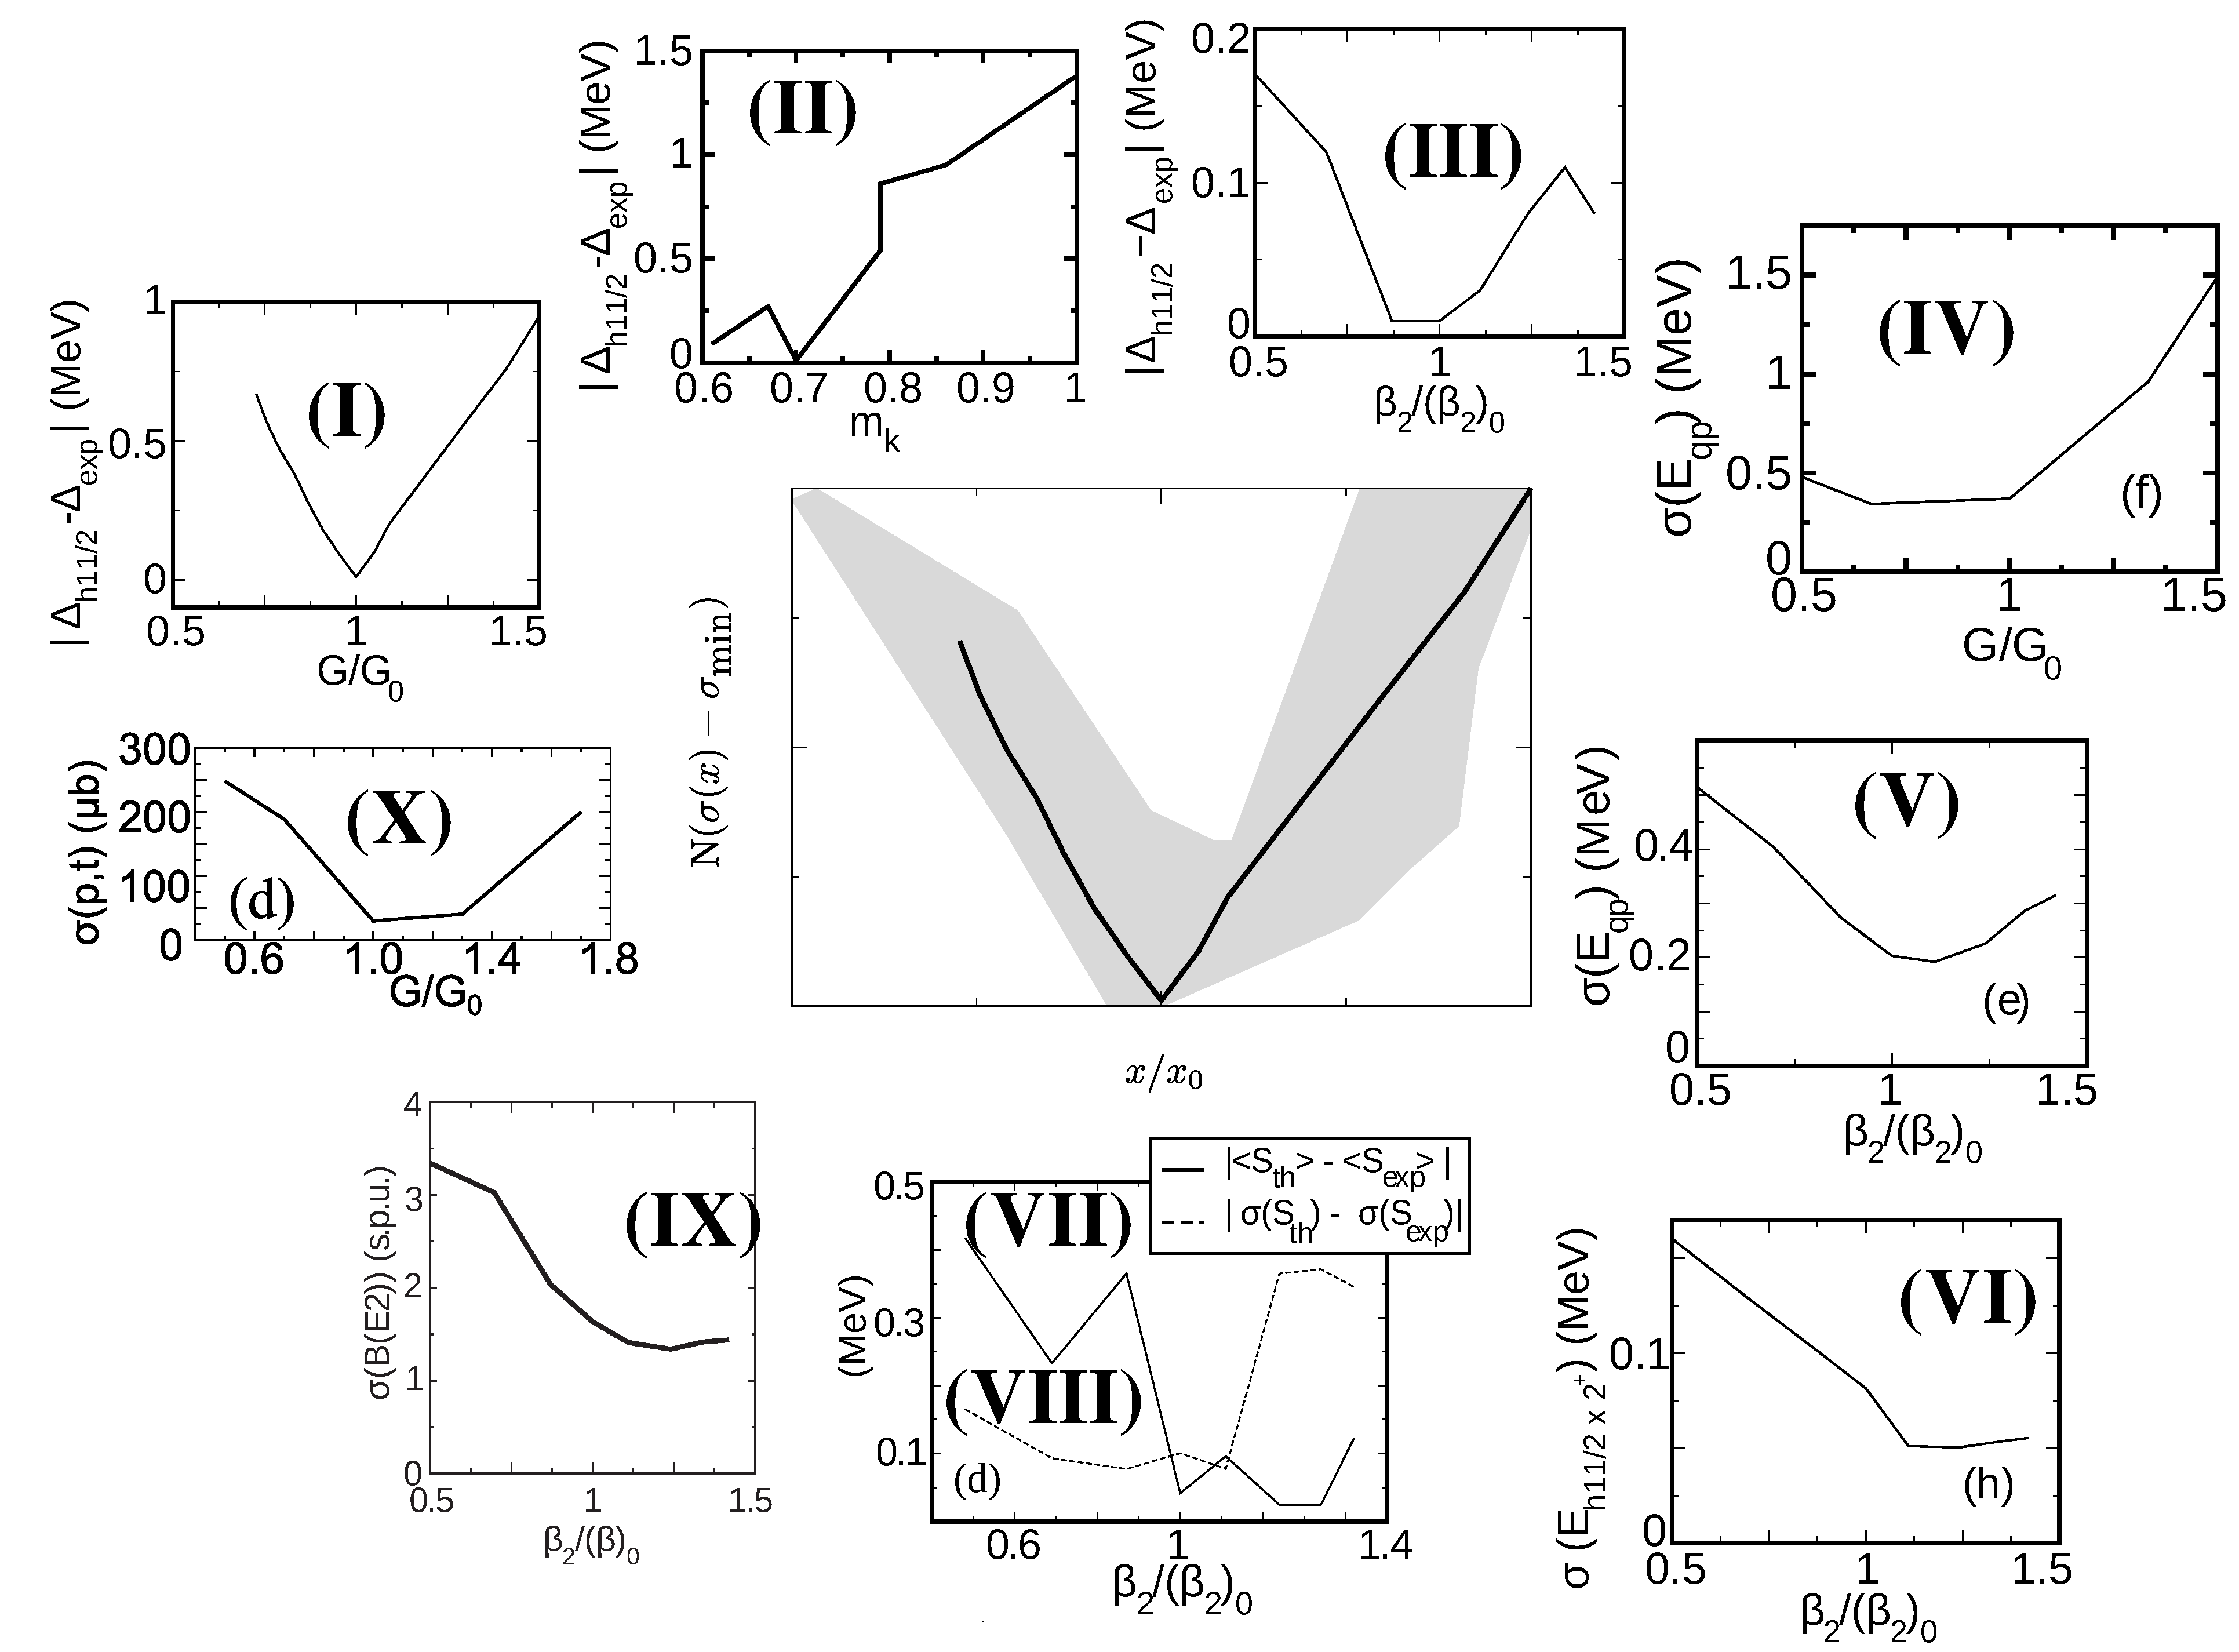
\includegraphics[width=18cm]{introduccion/figs/funnel_norm_tot_try_v3.pdf}}
\caption{Root mean square deviations $\sigma(x)$ between theoretical predictions and experimental values of the different structural properties which  characterize the open-shell nucleus $^{120}$Sn (see Table \ref{tab1.4.1} for the characterization of \textbf{(I)}--\textbf{(X)}; see also Fig. \ref{fig1.4.1}); (central figure) the bold black line and grey area provide a schematic representation of $\langle\sigma\rangle$ and associated fluctuations.}\label{fig1.4.1x}
\end{center}
\end{figure}


\begin{figure}[h!]
\begin{center}
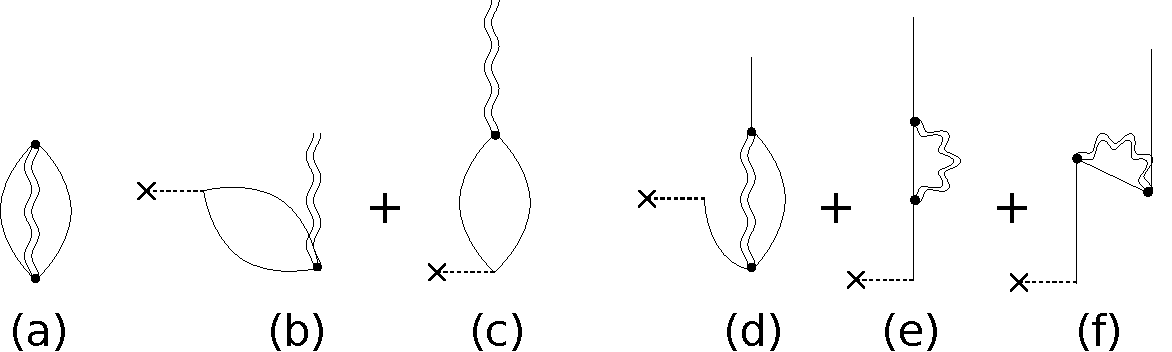
\includegraphics[width=\textwidth]{introduccion/figs/fig1_4_2.pdf}
\caption{Schematic representation of the NFT$_{\text{(s+r)}}$ diagrams at the basis of the characterization of a superfluid nucleus like e.g. $^{120}$Sn. \textbf{(a)} Nuclear structure (NFT$_{(\text{s})}$). Zero point fluctuations (ZPF) characterizing the nucleus ground state. Continuous lines describe quasiparticle (\textit{qp}) states, double wavy curves correlated two quasiparticle ($2qp$) vibrational modes. Because $\alpha^{\dagger}_{\nu}=U_\nu a^\dagger_\nu-V_\nu a_{\bar{\nu}}$ these modes encompass both particle-hole ($ph$) like vibrations, e.g. surface quadrupole vibrations, as well as correlated ($pp$) and ($hh$) monopole and multipole pairing vibrations. Intervening with an external field (cross followed by dashed line) one can excite (b) and (c) multipole ($ph$-like; inelastic scattering) and  pairing ($2p$-like, $2h$-like) vibrations (two-particle transfer) as well as (d)-(f) single-quasiparticle states.}\label{fig1.4.2}
\end{center}
\end{figure}

 \begin{table}
\begin{center}
\begin{tabular}{|c|c|c|c|c|}
\hline
  Observables  &  SLy4 &  $d_{5/2}$ shifted  & Opt. levels& Fig. \ref{fig1.4.1x} \\ 
\hline
$\Delta$ &  10  (0.7\%) &  10  (0.7 \%) & 50   (3.5 \%)&\textbf{(I)}, \textbf{(II),} \textbf{(III)}\\
 $E_{qp}$ & 190 (19\%)  & 160  (16\%)   & 45  (4.5 \%)& \textbf{(IV)}, \textbf{(V)}\\
 Mult.  splitt. & 50  (7\%) & 70  (10\%)    & 59  (8.4 \%)& \textbf{(VI)}\\
  $d_{5/2}$ strength (centr.) & 200  (20\%)  & 40  (4\%)   & 40  (4\%)& \textbf{(VII)} \\
$d_{5/2}$ strength (width) & 160  (20\%)  &75  (9.3\%)  &  8  (1\%)& \textbf{(VIII)}\\
$B(E2)$ & 1.4  (14\%) & 1.34  (13\%)   & 1.43  (14\%)& \textbf{(IX)}\\ 
$\sigma_{2n}(p,t)$ & 40 (2\%) & 40 (2\%) & 40 (2\%) &\textbf{(X)}\\
 %2n-transfer & 10 &10  & 10 \\ 
 \hline
\end{tabular}
\caption{Root  mean square deviation $\sigma$ between  the experimental data and the theoretical values expressed in keV for the pairing gap, quasiparticle energies, multiplet splitting, centroid and width of the  
$5/2^+$ low-lying single-particle strength distribution (Fig. \ref{fig6.2.3}). In single-particle units $B_{sp}$ for the $\gamma$-decay  (B(E2) transition probabilities) and in mb for $\sigma_{2n}(p,t)$ (Fig. \ref{fig8_2_4}). In brackets, 
the ratio $\sigma_{rel}=\sigma/L$ between $\sigma$ and the experimental  range $L$ of the corresponding quantities, is given: 1.4 MeV ($\Delta$), 1 MeV ($E_{qp}$), 700 keV (mult. splitting), 
1 MeV ($d_{5/2}$ centroid),  809 keV (=1730--921) keV;  $d_{5/2}$ width), 10 $B_{sp}$ (B(E2)), 2250 $\mu$b ($\sigma_{2n}(p,t)$)) is given. Columns 2,3, and 4 contain the results of NFT calculations making use of bare single-particle levels from Hartree-Fock with Sly4, same but for a 600keV shift towards the Fermi energy of the $\epsilon_{d_{5/2}}$ orbital, and optimal values of $\epsilon_j$ for all valence levels so that the dressed quasiparticle states provide the best fit to that data, respectively. In the last column reference to the corresponding diagrams shown in Fig. \ref{fig1.4.1x} are given. See also Fig. \ref{fig1.4.1}.}
\label{tab1.4.1}
\end{center}
\end{table}



\section{Coupling between intrinsic and relative motion}\label{appintroB}
In what follows, we consider the reaction
\begin{align}\label{eq2.5.1x}
a+A\rightarrow b+B,
\end{align}
within the framework of the semiclassical approximation\footnote{Assuming Eq. (\ref{eq2.5.1x}) to describe a transfer process induced by a heavy ion reaction with bombarding energy lying somewhat above the Coulomb barrier, the associated de Broglie reduced wavelength $\lambdabar=\sqrt{2mE}$ is much smaller than the nuclear dimension, and the relative motion can be described in terms of classical trajectories. On the other hand, the particle transfer process is described fully quantum mechanically. The coupling between the intrinsic (structure) nucleon motion and the relative motion associated with the recoil effect, is dealt with in terms of narrow wave packets. See e.g. \cite{Broglia:04a} and references therein.}.
In the center-of-mass system, the total Hamiltonian may be written
\begin{align}\label{eqintroB2}
H=T_{aA}+H_a+H_A+V_{aA}=T_{bB}+H_b+H_B+V_{bA},
\end{align}
in keeping with energy conservation. Within this context other, mixed, representations are possible.

One then solves the time-dependent Schr\"odinger equation 
\begin{align}
i\hbar\frac{\partial \Psi}{\partial t}=H\Psi,
\end{align}
with the initial conditions that the nuclei $a$ and $A$ are in their ground states, and where the relative motion is described by a narrow wavepacket of rather well defined impact parameter and velocity.


We expand $\Psi$ on (stationary) channel wavefunctions 
\begin{align}
\Psi=\sum_{\beta}c_\beta\left(\left(\mathbf r_\beta-R_\beta\right)\right)\Psi_\beta e^{-iE_\beta t/\hbar},
\end{align}
where
\begin{align}
\Psi_\beta (t)=\Psi_m^b(\xi_b)\Psi_n^B(\xi_B)\exp(i\delta_\beta).
\end{align}
The index $\beta$ labels both the partition of nuclei $(b,B)$ as well as the quantal states of the two nucleons ($m,n$).


The phase $\delta_\beta$ is defined as
\begin{align}
\delta_\beta=\frac{1}{\hbar}\left\{m_\beta \mathbf v_\beta(t)\cdot \left(\mathbf r_\beta-\mathbf R_\beta(t)\right)-\int_0^t\left(U_\beta\left(R_\beta(t')\right)-\frac{1}{2}m_\beta\mathbf v_\beta(t')^2\right)\right\},
\end{align}
 where an extra phase has been added to eliminate, as far as possible, the diagonal matrix elements in the coupled equations.
The phase factor $\exp(i\delta_\beta)$ acting on the channel wavefunction is essentially a Galilean transformation (see jagged ``phonon'' in insets to Figs.  \ref{figintro2} and \ref{figintro3}).



The function $c_\beta$ can be expressed as
\begin{align}
c_\beta=a_\beta(t)\chi_\beta(\mathbf r_\beta-\mathbf R_\beta(t),t)
\end{align}
product of an amplitude $a_\beta$ of asymptotic values ($t=\pm\infty$, 0 or 1), and a normalized shape (wavepacket) function, $R_\beta(t)$ being the relative motion elastic trajectory.


Properly combining the above quantities and making use of the time-dependent Schr\"odinger equation one obtains 
\begin{align}
i\hbar\sum_{\beta}\dot a_\beta(t)\langle\Psi_\xi|\Psi_\beta\rangle_{\mathbf R_{\xi\gamma}}e^{iE_\beta t/\hbar}=\sum_{\gamma}\langle\Psi_\xi|V_\gamma-U_\gamma(r_\gamma)|\Psi_\gamma\rangle_{\mathbf R_{\xi\gamma}}a_\gamma(t)e^{iE_\beta t/\hbar},
\end{align}
where
\begin{align}
f(\mathbf R)=\langle\Psi_\xi|V_\gamma-U_\gamma(r_\gamma)|\Psi_\gamma\rangle_{\mathbf R}
\end{align}
are the formfactors, and
\begin{align}
g(\mathbf R)=\langle\Psi_\xi|\Psi_\beta\rangle_{\mathbf R}
\end{align}
the \textit{overlaps between the intrinsic channel wavefunctions}.



The coupled equations can be written in a more compact form by introducing the adjoint channel wavefunction 
\begin{align}
\omega_\xi=\sum_{\gamma}g_{\xi\gamma}^{-1}\Psi{\gamma},
\end{align}
where $g^{-1}$ is the reciprocal of the \textit{overlap matrix}
\begin{align}
g_{\xi\gamma}=\langle\Psi_\xi|\Psi_\gamma\rangle.
\end{align}
Thus
\begin{align}
(\omega_\xi,\Psi_\beta)=\delta(\xi,\beta),
\end{align}
and
\begin{align}
i\hbar\dot a_\beta(t)=\sum_{\gamma}\langle\omega_\beta|V_\gamma-U_\gamma|\Psi_\gamma\rangle_{\mathbf R_{\beta\gamma}}e^{(E_\beta-E_\gamma)t/\hbar}a_\gamma(t).
\end{align}
Consequently, the proper tunneling Hamiltonian is obtained by a \textit{basis orthogonalization process}\footnote{Cf. with Eq. (\ref{eq3.C.1}) and following discussion, in connection with the derivation of the Cooper pair tunneling Hamiltonian (\cite{Cohen:62}) between two weakly cupled superconductors (Josephson junction).}. These coupled equations, being first order in time, can be solved knowing the initial conditions at time $t=-\infty$,
\begin{align}
a_\gamma(-\infty)=\delta(\gamma,\alpha),
\end{align}
where $\alpha$ labels the entrance channel, that is, the nuclei $a$ and $A$ in their ground state. The cross section for the reaction $\alpha\rightarrow\beta$ is
\begin{align}
\left(\frac{d\sigma}{d\Omega}\right)_{\alpha\rightarrow\beta}\sim\left|a_\beta(t=+\infty)\right|^2.
\end{align}



\section{Nuclear Field Theory for pedestrians}\label{appintroA}
\epigraph{The diagrams were intended to represent physical processes and the mathematical expressions to describe them\dots I would see electrons going along, being scattered at one point\dots emitting a photon and the photon goes over there\dots I thought that if they really turn out to be useful it would be fun to see them in the pages of Physical Review}{R. P. Feynman}
Nuclear Field Theory (NFT) was tailored after Feynman's graphical version of quantum electrodynamics (QED). It is then natural that in discussing NFT, analogies with QED are recurrent.   Arguably, as a consequence of special relativity which put an end to the concept of ether, the field-free and matter-free vacuum was rightly considered as \textit{bona fide} empty space. The advent of quantum mechanics changed this situation, the vacuum becoming populated. In quantum mechanics an oscillator, for example, cannot be at rest. The oscillatory nature of the radiation field requires zero point fluctuations (ZPF) of the electromagnetic fields in the vacuum state of lower energy. The occupation of the negative kinetic energy electron states and the subsequent calculation of the cross section for pair creation by photons, contributed another step in the understanding of the QED vacuum, let alone the Lamb shift\footnote{In high energy collisions and accelerator laboratories some of the original beam energy can be consumed by ripping electron-positron pairs out of the vacuum (\cite{Bruce:07}).}.


When the fields are expressed in terms of creation and annihilation operators, the interaction between  fermion and boson fields is proportional to the product of two fermion creation or destruction operator $a^\dagger$ or $a$, and of one boson operator $\Gamma^\dagger$ or $\Gamma$: e.g. $a^\dagger_{\nu'}a_\nu\Gamma_\alpha^\dagger$, (see Fig. \ref{figintroA1}). That is,  bilinear in the fermion fields and linear in the boson fields.

\begin{figure}
\centerline {
\includegraphics*[width=12cm]{introduccion/figs/figintroA1}
}
\caption{Oyster diagrams describing the correlation of the nuclear ground state associated with the ZPF of  collective particle--hole--like excitations. In (a) we show two of such diagrams. In (b) and (c) we display a symmetrized (boson exchange), and antisymmetrized  (fermion exchange) correction to (a), while  (d) contains a simultaneous boson and fermion exchange. In all the diagrams shown, only ground state correlation vertices are present. They are connected with the $Y^\alpha_{k_i}$--components ($\epsilon_k>\epsilon_F, \,\epsilon_i\le\epsilon_F$) of the RPA wavefunction describing the collective mode (wavy line). While this is so for any time ordering, i.e., the sequence with which the particle-vibration coupling vertex (black dots) appear in the case of the processes shown in (a) and (b), this is not the case in connection with processes shown in (c) and (d) as can be seen from the corresponding diagrams (c') and (d') shown in the inset. Because of Pauli principle between particles (holes) present and those involved in the collective modes, the harmonic approximation has to be corrected. This is diagramatically reflected by the presence of scattering vertices.}
\label{figintroA1}
\end{figure}
\begin{figure}
\centerline {
\includegraphics*[width=10cm]{introduccion/figs/fig1_7_2}
}
\caption{Some of the possible outcomes resulting from acting with an external single--particle field, i.e. that associated with inelastic processes (represented by a horizontal dashed line starting with a $\times$) on the ZPF of a nucleus ground state associated with particle-hole correlated vibrations. Within this context one returns to the question of  renormalization mentioned in the text (see also \cite{Idini:15}, \cite{Broglia:16}, \cite{Barranco:17}; see also Sect. \ref{C6S4}) The diagrams of the first row result by intervening the virtual process shown in Fig. \ref{figintroA1} (c) and eventual time orderings. Similar for those of the second row but in connection with diagram (d) of Fig. \ref{figintroA1}. The boxed processes correspond to particle self--energy (first row) and vertex correction (second row). Reversing the sense in which the fermions (arrowed lines) circle the loop from anticlockwise to clockwise, one obtains two new graphs. The  set of processes obtained in this way are shown in the third and last row, and constitute a sum rule conserving set of diagrams (see first row Fig. \ref{fig1.0.9}).}
\label{figintroA2}
\end{figure}
\clearpage
\begin{figure}[h!]
\centerline {
\includegraphics*[width=10cm]{introduccion/figs/figintroA3}
}
\caption{ZPF associated with the pair addition mode taking into account the interweaving of nucleons with density modes. The processes boxed in (g), (k) and (o), are associated with the induced pairing interaction (medium polarization effects; (p), (q), (r)) resulting from the exchange of density modes between nucleons moving in time reversal states, including also vertex corrections. The two--nucleon stripping and pickup external field is labeled by a dashed horizontal line which starts with a $\times$. The possibility of using pairing vibrational modes as intermediate bosons contributing to the induced pairing interaction, not only in $^1S_0$ channels but also in other channels (multipole modes) is discussed in App. \ref{App6G}. In particular, in connection with the possible presence of ``vortex--like'' pair addition modes, in exotic, halo nuclei, with $J^\pi=1^-$ and $\beta=+2$ quantum numbers, connected also with the pygmy dipole mode in $^{11}$Li (see e.g. \cite{Broglia:19} and refs. therein).}
\label{figintroA3}
\end{figure}
\clearpage

A detailed graphical NFT treatment of the vacuum has an important consequence concerning the probing of nuclear structure with reactions. By intervening it with an external field one will excite the modes whose properties can be  compared with experimental findings.

In other words, if one is in doubt of which are the properly dressed elementary, physical modes of excitation, one should find out how to specifically excite the  mode in question, by acting with an external field on the ZPF of the vacuum (Hawking-like radiation\footnote{\cite{Barranco:19b}.}; see also Sect. \ref{S6.6} in particular Fig. \ref{fig6.6.2}). That is,  carry out an NFT-like \textit{gedankenexperiment}\footnote{H. C. \O{}ersted, circa 1812.} as in Fig. \ref{figintroA2} for $p-h$-vibrations and in Fig. \ref{figintroA3} regarding pairing vibrations. Because the corresponding processes deal  with physical states, they translate with ease into a laboratory setup. In keeping with the fact that the vacuum contains all the information (right physical degrees of freedom) of the quantal system under study. Forcing virtual processes associated  with vacuum ZPF to become real, one is guaranteed to get, in each instance, the real, dressed, physical particle. 

The fact that one can treat fully quantum mechanically and on equal footing both structure and reaction processes is apparent from these figures and considerations\footnote{Full fledge embodiments being found in e.g. Figs. \ref{fig1.9.2}, \ref{fig1.9.3} and  \ref{fig6.6.2}.}. Thus unification of structure and reactions, and dressing of energies, vertices (interactions) and formfactors (single--particle radial wavefunctions and associated transition densities), results in a single vacuum correlated state (e.g. Figs. \ref{figintroA1} and \ref{figintroF2}). Vacuum states which through its fluctuations, reflect both single--particle, normal and abnormal (pairing) density vibrations and their interweaving.  It also indicates the  set of specific probes which make  these virtual states to collapse into on--the--energy shell states, providing the corresponding physical information to the   outgoing particles, also photons, which eventually interact with the corresponding detectors (e.g. Figs. \ref{figintroA2}, \ref{figintroA3} and \ref{fig1.9.2}). Structure and reaction processes free of non--orthogonality, overcompleteness and Pauli violation contributions.


Summing up, the last line of Fig. \ref{figintroA2} displays, together with the corresponding time orderings, the lowest order self--energy and vertex correction renormalising vibrational states. It thus gives rise to the physical collective vibrations whose properties can be directly compared with the experimental findings. In other words, the processes shown in the last line of   Fig. \ref{figintroA2} imply that the elementary modes participating in the virtual states have to display, exception made for energy (off-shell modes) the same properties of the physical, dressed (renormalized), on-shell modes whose properties can be directly compared with experiment\footnote{Examples of these processes in the case of giant resonances are found in \cite{Bortignon:81,Bertsch:83} and references therein. For low-lying states see \cite{Barranco:04}.} (renormalized NFT). This is because one can, through an experiment
force such virtual states to become real (on-shell) on short call.

Let us now provide an introduction to NFT for pedestrians and see how the above considerations become concretely implemented\footnote{For details we refer to \cite{Bortignon:77} and refs. therein.}
\subsection[The concept of elementary modes of excitation]{The concept of elementary modes of excitation\protect\footnote{\cite{Bes:77}}}\label{C1S7.1}
The Hamiltonian of a many--body system of noninteracting particles, bosons or fermions, can be written as
\begin{align}\label{eqC1A1}
H=\sum_iH_i,
\end{align}
where the summation is over all the particles of the system and where each $H_i$ depends only on the variables of the $i$--th particle. The single-particle Schr\"odinger equation is
\begin{align}\label{eqC1A2}
H_i\psi_k(\mathbf r_i)=\epsilon_k \psi_k(\mathbf r_i),
\end{align}
where $\epsilon_k$ is the single--particle energy eigenvalue and 
\begin{align}\label{eqC1A3}
\psi_k(\mathbf r_i)\equiv\bra{\mathbf r_i}a_k^\dagger\ket{0}
\end{align}
is the corresponding wave function. The operator $a_k^\dagger$ creates a particle in the state $k$ when acting in the vacuum state $\ket{0}$. The energy levels of the system are given by the equation
\begin{align}\label{eqC1A4}
E_n=\sum_k n_k\epsilon_k,
\end{align}
the corresponding eigenstates being
\begin{align}\label{eqC1A5}
\ket{n}=\prod_k\frac{(a_k^\dagger)^{n_k}}{\sqrt{n_k!}}\ket{0},
\end{align}
where $n_k=0$ or 1 in the case of fermions and $n_k=0,1,2,\dots$ in the case of bosons.

We now  consider a system of interacting particles. The Hamiltonian will in this case be
\begin{align}\label{eqC1A6}
H=\sum_i H_i+\frac{1}{2}\sum_{i,j}H_{ij},
\end{align}
where $i,j$ label the co--ordinates of the $i$--th and $j$--th particle.

In some cases it is possible to recast the two--body Hamiltonian in the form
\begin{align}\label{eqC1A7}
H=\sum_\tau H'_\tau,
\end{align}
with the associated Schr\"odinger equation
\begin{align}\label{eqC1A8}
H'_\tau\psi_\tau(\zeta)=\epsilon_\tau \psi_\tau(\zeta),
\end{align}
$\zeta$ representing a general variable (e.g. the single-particle coordinate, the gap parameter, the shape of the nucleus, etc.). The wave function $\psi_\tau(\zeta)$ is the $\zeta$-coordinate representation of the eigenstate $\alpha_\tau^\dagger\ket{\tilde 0}$. The operator $\alpha_\tau^\dagger$ creates an excitation with the quantum number $\tau$ when acting in the state $\ket{\tilde 0}$, the correlated vacuum of all the excitations $\tau$.



The energy of the levels of the system, or at any rate of the most important
ones to determine the physical response of it to external probes can be written
in the form
\begin{align}\label{eqC1A9}
E_m=\sum_{\tau}n_\tau \epsilon_\tau.
\end{align}
The corresponding eigenstate can be written in the same way as before, \textit{i.e.}
\begin{align}\label{eqC1A10}
\ket{n}=\prod_\tau\frac{(\alpha_\tau^\dagger)^{n_\tau}}{\sqrt{n_\tau!}}\ket{\tilde 0}.
\end{align}
Additivity features similar to (\ref{eqC1A9}) hold for other physical quantities, \textit{i.e.}
\begin{align}\label{eqC1A11}
\braket{n|\mathcal O|m}=\sum_{\tau}A_\tau\sqrt{n_\tau} \delta(n_\tau,m_\tau+1),
\end{align}
where
\begin{align}\label{eqC1A12} O=\sum_{\tau}A_\tau \alpha_\tau^\dagger
\end{align}
is the operator which specifically excites the eigenstates described by $\psi_\tau(\xi)$.
Because the excitation energies $E_m$ and observables $\left|\braket{m'|\mathcal O|m}\right|^2$ (e.g. absolute two--particle transfer cross--section, electromagnetic-transition probabilities, etc.) are
linear combinations of $\epsilon_\tau$ and $A_\tau$, respectively, the eigenstates with energy $\epsilon_\tau$
and associated observable $A_\tau$ are called the \textit{elementary excitations of the system}.


The elementary modes of excitation  of a many-body system  represent a generalization of  the idea of normal modes of vibration.
They provide the building blocks of the excitation spectra, giving  insight  into the  deep nature  of the system one is studying, aside from allowing 
for an economic description  of complicated spectra in terms of a gas of, as a rule, weakly interacting bosons and fermions. In the nuclear case 
they correspond to dressed particles and empirically renormalised vibrations (rotations).

There lie two ideas behind the concept of elementary modes of excitation\footnote{This concept was introduced by Landau (\cite{Landau:41}) to describe the spectrum of He II. It was subsequently utilized by Bohr and Mottelson (\cite{Bohr:75}) to obtain a unified description of the nuclear spectrum.}. First, that one does not need to be able to calculate the total binding
energy  of a nucleus to accurately describe the low energy excitation spectrum, in much the same way in which one can calculate 
the normal modes of a metal rod not knowing how to  calculate its total cohesive energy.
The second idea is that low-lying states ($\hbar \omega \ll \epsilon_F \ll BE$, i.e. binding energy) are of a particularly simple
character, and  amenable to a simple treatment, their
interweaving  being carried out at profit, in many cases,  in perturbation theory
\footnote{More precisely, and in keeping with  the fact that (quasi)
boson degrees of freedom have to decay through linear particle-vibration 
coupling vertices of strength $\Lambda$ into their fermionic components to interact with another vibrational mode,
the interweaving between the variety of many-body components dressing a single-particle state 
or a collective vibration will be described at profit in terms of an arrowed matrix which, assuming perturbation theory
to be valid, can be transformed, neglecting contributions of the order of $\Lambda^3$ or higher, into a co-diagonal matrix, namely a matrix 
whose non-zero elements are $(i,i-1)$ and $(i,i+1)$,  aside from  the diagonal ones $(i,i)$.}. 
Within this context it is  necessary to have a microscopic description 
of the ground  state of the system  which ensures that it acts as the vacuum state 
$|\tilde0\rangle  $ of the elementary modes of excitation. In other words $a_{\nu}|\tilde 0 \rangle   = 0, \Gamma_{\alpha} |\tilde 0\rangle   =0$, where
$a^+_{\nu}|\tilde 0 \rangle   = |\nu\rangle  $ and , $\Gamma^+_{\alpha} |\tilde 0\rangle   =|\alpha\rangle  $ represent a single-particle and a one-phonon state.
This   implies, in keeping 
with the indeterminacy  relations\footnote{The quantities $I$ and $N$   are the angular momentum and particle number, conjugate variables to the Euler and gauge angles $\Omega$, $\phi$ respectively.} $\Delta x \Delta p \geq \hbar/2$, $\Delta I \Delta \Omega \geq 1$, $\Delta N \Delta \phi \geq 1$, etc.,  that $|\tilde 0\rangle   = |0\rangle  _F |0\rangle  _B$
displays the  quantal zero point fluctuations (ZPF) of the many--body system under study.

Within the framework of nuclear field theory (NFT) used below, in which single-particle (fermionic, F) and vibrational
(bosonic, B) elementary modes of excitation are to be calculated within the framework of HFB and QRPA
respectively\footnote{Hartree-Fock (HF) and Random Phase (RPA) approximation extended to open shell superfluid nuclei. Namely Hartree-Fock-Bogoliubov and Quasi Random Phase Approximation.}, $|\tilde 0\rangle  $ must display the associated ZPF (cf. App. \ref{App1.E}). In particular for (harmonic) vibrational modes the indeterminacy relation achieves its lowest possible value 
$\Delta x \Delta p = \hbar/2$, the associated zero point energy amounting to $\hbar \omega/2$
for each degree of freedom. For example 5$\hbar \omega/2$ for quadrupole vibrations, 
$\hbar \omega$ being the energy of the collective vibrational mode under consideration. 




An illustrative example of the above arguments is provided by the low-lying quadrupole vibrational state of $^{120}$Sn. 
Diagonalizing the effective SLy4 Skyrme interaction\footnote{\cite{Ring:80}.} in QRPA leads to a value of $B(E2)$
(890 $e^2$ fm$^2$) which is about a factor of 2 smaller than experimentally observed (2030 $e^2$ fm$^2$). 
Taking into account  renormalisation effects in NFT, 
namely in a conserving  approximation (self-energy and vertex corrections),   one obtains a value of 2150 e$^2$ fm $^2$. 


If the collective phonons are not the main object  of the study, but are to be used to cloth the single-particle states 
and give rise to the induced pairing interaction, one can make 
use of phonons which account for the experimental findings (renormalization\footnote{\cite{Idini:15,Broglia:16,Barranco:17}.})\footnote{As already mentioned, with the help of experimental probes which couple weakly to the nucleus,
i.e. in such a way that the system can be expressed in terms of the properties
of the excitation in the absence of probes (see however Sect. \ref{S6.5.4}), it has been possible to identify, among others, the
following elementary excitations in systems around closed shells:
\begin{enumerate}[a)]
\item single--particle and --holes,
\item shape vibrations,
\item spin and isospin vibrations and charge exchange modes,
\item pairing vibrations.
\end{enumerate}
Away from closed shells one has to add to the above modes:
\begin{enumerate}[a)]
\setcounter{enumi}{4}
\item rotations in 3D--space (e.g. quadrupole rotations)
\item rotations in gauge space (pairing rotations).
\end{enumerate}
Different probes have been utilized in the process of the identification of the different modes. In particular two-neutron transfer reactions induced by tritons
and protons have played a central role in unraveling the basic features of the pairing modes.}.




 
\subsection{NFT rules and applications}\label{Sect1.7.2}
A field theory can be formulated in which the nuclear elementary modes of
excitation play the role of the free fields and in which their mutual interweaving takes place through four-point ($v$) as well as three-point particle-vibration coupling vertices\footnote{\cite{Bes:74,Broglia:76,Bohr:75,Mottelson:76}.}.
This theory provides a graphical perturbative approach to obtain the exact
solution of the many-body nuclear-structure problem in the product basis $\psi_\tau(\zeta)\psi_\eta(\Delta)\dots\psi_\gamma(\Gamma)$




In what follows we state and apply the nuclear-field-theory rules, to calculate the interactions between the nuclear free fields and the reaction processes
between the resulting physical states making use of a simple model. \subsubsection{Schematic model}
The model considered consists of two single-particle levels, each with pair degeneracy\footnote{It is of notice the difference of a factor of 2 in the degeneracy of each level as compared to Sect. 2 of \cite{Bortignon:77} in which case it is $2\Omega$. This is in keeping with the fact that, as a rule, $\Omega=(2j+1)/2$. See also Eq. (\ref{eqC1A86}) and related discussion. \label{fnlabel}} $\Omega$ and with a schematic monopole particle-hole interaction coupling the particles in the two levels.

The total Hamiltonian is equal to
\begin{align}\label{eqC1A13} 
H=H_{sp}+H_{TB}
\end{align}
where
\begin{align}\label{eqC1A14} 
H_{sp}=\frac{\epsilon}{2}N_0,\quad\quad N_0=\sum_{\sigma=\pm 1,m}\sigma a^{\dagger}_{m,\sigma}a_{m,\sigma},
\end{align}
and
\begin{align}\label{eqC1A15} 
H_{TB}=-\frac{V}{2}\left(A^\dagger A+AA^\dagger\right),\quad\quad A^\dagger=\sum_m a^\dagger_{m,1}a_{m,-1}.
\end{align}


The index $\sigma$ (=$\pm1$) labels the two levels, while $m$ labels the degenerate states within
each level. The strength of the monopole coupling is denoted  $V$ and the
energy difference between the two levels  $\epsilon$. 
The matrix element of (\ref{eqC1A15}) is given by
\begin{align}\label{eqC1A16} 
\braket{m,1;m',-1|H_{TB}|m'',1;m''',-1}=-V\delta(m,m')\delta(m'',m''').
\end{align}
\subsubsection{Field--theoretical solutions}
 The boson fields are defined through the random-phase
approximation, in terms of particle-hole excitations. The basis utilized to
describe the nuclear systems is a product of the different free fields. 
The closed-shell system of the schematic model under consideration corresponds to the lowest ($\sigma = - 1$) level filled with $\Omega$ particles, while the upper
($\sigma =  1$) level remains empty. The basis particle and hole states are obtained
by adding or removing a single particle to/from this closed-shell configuration.
The corresponding wave functions and energies, which should include the
Hartree-Fock corrections (see Fig. \ref{figintro4} (b), (c)) generated by the residual interaction\footnote{The Hartree--Fock energy associated with the Hamiltonian (\ref{eqC1A13}) can be obtained
from the linearization relation $[H,a_{\sigma,m}^\dagger]=E(m,\sigma)a^\dagger_{\sigma,m}$ acting on the Hartree-Fock
vacuum (see Eq. (\ref{eq0.1.15})), which in this case coincides with the single-particle vacuum defined by
 $a^\dagger_{m,-1}\ket{0}=a_{m,1}\ket{0}=0$.}, are
 \begin{align}\label{eqC1A17} 
\left\{\begin{array}{l}
 \ket{m,1}=a^\dagger_{m,1}\ket{0},\quad E(m,1)=\frac{1}{2}(\epsilon+V),\\ 
\ket{m,-1}=a_{m,-1}\ket{0},\quad E(m,-1)=\frac{1}{2}(\epsilon+V).
\end{array} \right.
 \end{align}
Thus the unperturbed energy for producing a particle-hole excitation with
respect to the ground state is
 \begin{align}\label{eqC1A18} 
\epsilon'=E(m,1)+E(m,-1)=\epsilon+V.
 \end{align}
 \begin{figure}
 \centerline {
 \includegraphics*[width=4cm]{introduccion/figs/fig18}
 }
 \caption{Graphical representation of the amplitude of the collective phonon (wavy line) on a given particle-hole excitation ($(m,1),(m,-1)$). This amplitude can be written in terms of the interaction vertex denoted  $\Lambda_i$, and the energy denominator $\omega_i-\epsilon'$. The particles (holes) are depicted by upward-- (downward--) going arrowed lines. Time is assumed to run upwards.}
 \label{figC1A1}
 \end{figure}
The contribution $V$ in (\ref{eqC1A18}) is the Hartree--Fock contribution to the particle--hole excitation.

If we define the creation operator of the normal modes as
 \begin{align}\label{eqC1A19} 
\beta^\dagger_\nu=\sum_m \lambda_m^\nu a_{m,1}^\dagger a_{m,-1},
 \end{align}
the linearization equation (see Eq. (\ref{eq0.1.14})),
 \begin{align}\label{eqC1A20} 
[H,\beta_\nu^\dagger]=\omega_\nu\beta^\dagger_\nu,
 \end{align}
yields
 \begin{align}\label{eqC1A21} 
\left\{\begin{array}{l}
 \omega_1=\epsilon'-V\Omega,\\ 
\omega_\nu=\epsilon'\quad (\nu=2,3,\dots,\Omega).
\end{array} \right.
 \end{align}
Utilizing (\ref{eqC1A20}) and the normalization condition
 \begin{align}\label{eqC1A22} 
[\beta_\nu,\beta^\dagger_{\nu'}]=\delta(\nu,\nu'),
 \end{align}
we obtain for the amplitudes associated with the lowest mode
 \begin{align}\label{eqC1A23} 
\lambda_m^1=\frac{1}{\sqrt{\Omega}}.
 \end{align}
One can also write this amplitude as the ratio between a coupling matrix
element and an energy denominator, i.e.
 \begin{align}\label{eqC1A24} 
\lambda_m^1=\frac{\Lambda_1}{\omega_1-\epsilon'}.
 \end{align} 
From (\ref{eqC1A21}), (\ref{eqC1A23}) and (\ref{eqC1A24}) we obtain
 \begin{align}\label{eqC1A25} 
\Lambda_1=-V\sqrt{\Omega},
 \end{align}
which is the strength with which a particle~hole excitation $(m, 1; m, -1)$
couples to the collective phonon (see Fig. \ref{figC1A1}). This can also be seen by calculating
the matrix element of the interaction Hamiltonian (\ref{eqC1A15}) between the normal
modes and the single particle-hole state
 \begin{align}\label{eqC1A26} 
\Lambda_\nu=\braket{n_\nu=1|H_{TB}|m,1;m',-1}=-V\sqrt{\Omega}\,\delta(m,m')\,\delta(\nu,1).
 \end{align}
Note that the particle--vibration coupling strengths associated with the other
normal modes lying at an energy $\epsilon'$ (see (\ref{eqC1A21})) are equal to zero. The exact solution of (\ref{eqC1A13}) is reproduced by utilizing
as the basic degrees of freedom both the vibrations (see (\ref{eqC1A21})) and the particles
(see (\ref{eqC1A17})) coupled through the interactions (\ref{eqC1A16}) (four--point vertex) and (\ref{eqC1A26}) (particle-vibration coupling). A significant
part of the original interaction has already been included in generating the
collective mode (\ref{eqC1A21}). This implies that the rules for evaluating the effect of
the couplings (\ref{eqC1A16}) and (\ref{eqC1A26}) between fermions and bosons, involve a number of restrictions as compared with the usual rules of perturbation theory that
are to be utilized in evaluating the effect of the original interaction (\ref{eqC1A15}) acting
in a fermion space. They read as follows:
\begin{enumerate}[I)]
\item In initial and final states, proper diagrams involve collective modes
and particle modes, but not any particle configuration that can be replaced by
a combination of collective modes. This restriction permits an initial state
comprising the configuration ($n_\nu =1;m$), but excludes ($m', 1; m',-1; m,1$).
\item The couplings (\ref{eqC1A16}) and (\ref{eqC1A26}) are allowed to act in all orders to
generate the different diagrams of perturbation theory; the restriction I) does
not apply to internal lines of these diagrams.
\item The internal lines of diagrams are, however, restricted by the exclusion of diagrams in which a particle--hole pair is created and subsequently
annihilated without having participated in subsequent interactions.
\item The energies of the uncoupled particle and phonon fields are to be
calculated by utilizing the Hartree-Fock approximation (see eq. (\ref{eqC1A17})) and the
RPA (see eq. (\ref{eqC1A21})), respectively. The contributions of all allowed diagrams are
evaluated by the usual rules of perturbation theory.
\end{enumerate}

We note that the external fields acting on the system are allowed to create
any state which may generate the different diagrams of perturbation theory.
The corresponding matrix elements should be weighted with the amplitude of
the component through which the final state is excited.



The above rules are also valid for those situations which cannot be treated
in perturbation theory and where a full diagonalization is called for. Thus,
\textit{e.g}., when the system displays a spurious state (see Sect. \ref{C1S7sS3}).



In what follows we discuss the energy of the $2p-1h$--like excitations, simplest modes which can display spuriousity. We
distinguish between two types of states, namely
 \begin{align}\label{eqC1A27} 
\ket{n_i=1;m,1},\quad\left\{
\begin{array}{ll}
\omega_1=\epsilon'-V\Omega, &\Lambda_1=-\sqrt{\Omega}V\\
&(i=1;m=1,2,\dots,\Omega),  \\ 
\omega_i=\epsilon', &\Lambda_i=0\\
&(i=2,\dots,\Omega; m=1,2,\dots,\Omega),
\end{array} \right. 
 \end{align}
and
 \begin{align}\label{eqC1A28} 
\ket{m',1;m',-1;m,1},\quad\epsilon'\quad(m,m'=1,2,\dots,\Omega),
 \end{align}
 where as in (\ref{eqC1A27}) only the energy of the particle-hole excitation is given (see (\ref{eqC1A18})). 
The physical states are to be written as
 \begin{align}\label{eqC1A29} 
\ket{qm}=\sum_i\xi_{iqm}\ket{n_i=1;m,1},
 \end{align}
 
  \begin{figure}
 	\centerline {
 		\includegraphics*[width=13cm]{introduccion/figs/figalpha}
 	}
 	\caption{Schematic two--level model. Count of the states $\ket{m,1;m-1;m',1}$ in the case of $j=3/2$ and $\Omega=2j+1=4$. State (b) is not allowed because of Pauli principle. The states ((a),(e)), ((c),(f)) and ((d),(g)) are pairwise identical, in keeping with the indistinguishability of the particles. Thus, the states (a), (c) and (d) (equivalent (e), (f) (g)) exhaust the degrees of freedom of states of type (\ref{eqC1A28}). In other words, there are only $\Omega-1=3$ two-particle one-hole states in which the odd particle is in the state ($m',1$). It is of notice that all substates $m$ of levels $\sigma=\pm1$ are degenerate. One displays them equally spaced only for didactical purposes.}
 	\label{figalpha}
 \end{figure}
  \begin{figure}
  \centerline {
  \includegraphics*[width=12cm]{introduccion/figs/fig19}
  }
  \caption{Contributions to the interaction of a fermion and a collective boson $\omega_i$ to order $1/\Omega^4$. The secular equation $E-E^{(0)}=A\sum_na^n(-1)^n$ is given in terms of the quantities $A=4\Omega V^2/(3\epsilon'-2E)$ and $a=2V/(3\epsilon'-2E)$. The hatched circle stands for the four-point vertex (\ref{eqC1A16}) (see also Fig. \ref{figC1A4} (I)).}
  \label{figC1A2}
  \end{figure}
in keeping with the fact that (\ref{eqC1A28}) cannot be basis states according to rule I), but only intermediate
states. The quantities $\xi_{iqm}$ are the amplitudes of the physical state in the different components of the product basis of elementary excitations. Rule I) eliminates most of the double counting of two-particle, one-hole states. The model state contains $\Omega$ ``proper'' states of the form $\ket{n_i;m,1}$,  in which case the odd particle is in the state $(m,1)$. That is $\ket{n_1;m,1}$ ($\omega_1=\epsilon'-V\Omega$) and $\ket{n_i;m,1}$ ($\omega_i=\epsilon',\; i=2,\dots,\Omega$). However, there are only $\Omega-1$ two--particle, one-hole states in which the odd particle is in the state $(m,1)$ (Fig. \ref{figalpha}). Therefore, a spurious state remains in the spectrum based on elementary modes of excitation. In other words, allowing the quantum number $m$ to run over all possible $\Omega$-states, the  model space contains $\Omega^2$ states (one for each value of $m$), while the correct number is $\Omega(\Omega-1)$.


 
Thus the basis $\ket{n_1=1; m,1}$ contains $\Omega$ spurious states. Its origin can be
traced back to the violation of the Pauli principle.
To obtain the energy of $\ket{qm}$ we have to allow the states $\ket{n_1=1;m,1}$
to interact through the vertices (\ref{eqC1A16}) and (\ref{eqC1A26}) and generate all the different
perturbation theory diagrams (see rule II)) except those containing bubbles
(see rule III)).


The different graphical contributions calculated within the framework of the
Brillouin-Wigner perturbation theory are displayed in Fig. \ref{figC1A2}. There is only
one (diagonal) matrix element given by a single summation, which can be
carried to all orders in the interaction vertices\footnote{Concerning the proper expansion parameter see Sect. \ref{Sect1.7.4}, Eq. (\ref{eqC1A86}).}, and can be written as
 \begin{align}\label{eqC1A31} 
\nonumber X_{ii'}=A\sum_n&(-1)^na^n\delta(i,i')=\\
&=\frac{A}{1+a}\delta(i,i')\delta(n,1)=-K(E)(\sqrt{\Omega}V)^2\delta(i,i')\delta(i,1),
 \end{align}
where a and A are defined in the caption to the figure and
 \begin{align}\label{eqC1A32} 
K(E)=\left(\tfrac{3}{2}\epsilon'-E+V\right)^{-1}.
 \end{align}
The associated secular equation
 \begin{align}\label{eqC1A33} 
\left|(\omega_i-E)\delta(i,i')+X_{ii'}\right|=0
 \end{align}
is equivalent to the dispersion relations ($i=1$ and $i\neq1$)
 \begin{align}\label{eqC1A34} 
\frac{1}{K(E)}=\frac{\Lambda_i^2}{\frac{1}{2}\epsilon'+\omega_i-E}.
 \end{align}
Thus the energies of the system are determined by the equation
 \begin{align}\label{eqC1A35} 
E=\frac{1}{2}\epsilon'+\omega_i+\frac{\Lambda_i^2}{\tfrac{3}{2}\epsilon'-E+V}.
 \end{align}
It admits the two solutions
 \begin{align}\label{eqC1A36} 
E_{qm}=\left\{\begin{array}{l}
\frac{3}{2}\epsilon', \\ 
\\
\frac{1}{2}\epsilon'+\omega_1+V=\frac{3}{2}\epsilon'-\Omega V+V,
\end{array} 
\right.
 \end{align}
which agree with the exact value\footnote{The exact solutions can be  obtained  by noting that the operators $A^\dagger,A$ and $\frac{1}{2}N_0$ are generators of the $SU_2$ group (see \cite{Bortignon:77}).}.


Because $A=0$ for $i\neq 1$, there is no summation in (\ref{eqC1A29}) and
 \begin{align}\label{eqC1A37} 
\ket{qm}=N^2_{qm}\ket{n_1=1;m,1},
 \end{align}
where
 \begin{align}\label{eqC1A38} 
1=N^2_{qm}\left(1-\frac{\partial X_{11}}{\partial E}\right)=N^2_{qm}\left(1-\frac{\Omega V^2}{\left(\frac{3}{2}\epsilon'-E+V\right)^2}\right).
 \end{align}
For $E_{qm}=\frac{1}{2}\epsilon'+\omega_1+V$ we obtain
 \begin{align}\label{eqC1A39} 
 N^2_{qm}=\frac{\Omega}{\Omega-1},
 \end{align}
while for $E_{qm}=\frac{3}{2}\epsilon'$ the state is non--normalizable as the quantity in parentheses
in (\ref{eqC1A38}) is either negative ($\Omega>1$) or zero ($\Omega=1$).
The state defined by
 \begin{align}\label{eqC1A40} 
\ket{q,m}=\sqrt{\frac{\Omega}{\Omega-1}}\ket{n_1=1;m,1},
 \end{align}
and 
 \begin{align}\label{eqC1A41} 
E_{qm}=\frac{1}{2}\epsilon'+\omega_1+V=\frac{3}{2}\epsilon'-V(\Omega-1),
 \end{align}
\textit{exhausts the inelastic sum rule in agreement with the exact results.} Note
that (\ref{eqC1A40}) is specifically excited in inelastic processes, as can be seen by
direct inspection.
  \begin{figure}
  \centerline {
  \includegraphics*[width=12cm]{introduccion/figs/fig20}
  }
  \caption{Graphical representation of the different terms contributing to the matrix element of the inelastic operator $\sqrt{\Omega}\,A^\dagger$ up to order $1/\Omega^3$. Note that the different contributions b),c), etc. have a one--to--one correspondence with the different contributions to $E$ (see Fig. \ref{figC1A2}); $a=-2V/(3\epsilon'-2E),\,b=2\Lambda_1/(3\epsilon'-2E)$.}
  \label{figC1A3}
  \end{figure}
The external inelastic field can act in two ways, exciting either a particle--hole pair or a phonon, with amplitudes 
 \begin{align}\label{eqC1A42} 
\braket{m,1;m',-1|A_1^\dagger|0}=\delta(m,m'),
 \end{align}
and
 \begin{align}\label{eqC1A43} 
\braket{n_i=1|A_1^\dagger|0}=\sqrt{\Omega}\delta(i,1),
 \end{align}
respectively. The different graphical contributions to the inelastic-scattering
process are displayed in Fig. \ref{figC1A3}, and can again be summed to all orders in the
interaction vertices giving
 \begin{align}\label{eqC1A44} 
\braket{n_1=1;m,1|A_1^\dagger|m,1}=\sqrt{\Omega}+\frac{\Lambda_1}{\frac{3}{2}\epsilon'-E_{qm}+V}.
 \end{align}
For $E_{qm}=\frac{3}{2}\epsilon'$ this quantity is equal to zero. Thus, the corresponding states
do not carry any inelastic strength, a feature which is closely related to the
fact that they cannot be normalized and that they do not display any correlation energy\footnote{Note that, even if $N(E_{qm}=\epsilon_m)\rightarrow\infty$, the matrix elements associated with the different transitions tend to zero more rapidly and the final result converges and is equal
to zero as expected.}.
On the other hand, the matrix element associated with (\ref{eqC1A40}) is
 \begin{align}\label{eqC1A45} 
\braket{qm|A^\dagger|m,1}=\sqrt{\frac{\Omega}{\Omega-1}}\frac{\Omega-1}{\sqrt{\Omega}}=\sqrt{\Omega-1},
 \end{align}
value which agrees with the exact answer.
The results (\ref{eqC1A41}) and (\ref{eqC1A45}) can be traced down to Pauli--principle corrections. In fact, the state $\ket{n_i=1;m,1}$ has a nonvanishing matrix element,
implying a single particle-vibration coupling vertex, with the state $\ket{m,1;m,-1;m,1}$. This component, which is spurious, is removed by the different graphs displayed in Figs. \ref{figC1A2} and \ref{figC1A3}. \textit{The presence of the odd particle
$(m, 1)$ blocks the particle-hole excitation $(m,1; m,- 1)$ which was present in
the uncoupled system. Thus the system increases its energy by a quantity $V$.
The reduction of the inelastic amplitude from $\sqrt{\Omega}$ to $\sqrt{\Omega-1}$  also indicates
that there is one less particle-hole excitation responding to the external probe.}
\subsection{Spurious states}\label{C1S7sS3}
While the model space product of elementary modes of excitation discussed
in the last section contains $\Omega^2$ states, only $\Omega(\Omega-1)$ are physically possible,
the number of spurious states being $\Omega$.  On the other hand, the agreement
between the exact and the nuclear-field-theoretical results shows that the effects of those spurious states are eliminated from all the matrix elements associated with physical observables.


In what follows we show that, in fact, the spurious states are isolated in an
explicit way in  nuclear field theory\footnote{\cite{Broglia:76}}. Their energy coincides with the
initial unperturbed  energy, while all physical operators have zero off--diagonal
matrix elements between any physical state and a spurious state, in particular
the unit operator, which measures the overlap of the two types of states.
For this purpose we use again a schematic model consisting in a number, $\Omega$,
of single--particle levels in which particles interact by means of a ``monopole''
force,
 \begin{align}\label{eqC1A46} 
H=H_{sp}+H_{int},
 \end{align}
where
 \begin{align}\label{eqC1A47} 
H_{sp}=\frac{1}{2}\sum_{m=1}^\Omega\epsilon_m\left(a^\dagger_{m,1}a_{m,1}-a^\dagger_{m,-1}a_{m,-1}\right),
 \end{align}
and
 \begin{align}\label{eqC1A48} 
H_{int}=-VA^\dagger A,
 \end{align}
with
 \begin{align}\label{eqC1A49} 
 A^\dagger=\sum_{m=1}^\Omega a^\dagger_{m,1}a_{m,1}.
 \end{align}

The energy of the i-th phonon is determined by the RPA dispersion relation (see rule IV)) 
 \begin{align}\label{eqC1A50} 
\sum_{m=1}^{\Omega}\frac{1}{\epsilon_m-\omega_i}=\frac{1}{V}.
 \end{align}
The eigenfunction corresponding to the different modes is 
 \begin{align}\label{eqC1A51} 
\ket{n_i=1}=\sum_m\frac{\Lambda_i}{\epsilon_m-\omega_i}a^\dagger_{m,1}a_{m,-1}\ket{0}.
 \end{align}


The particle-vibration coupling constant is given by 
 \begin{align}\label{eqC1A52} 
\Lambda_i=-\braket{n_i=1|H_{int}|m,1;m',-1}=\left[\sum_m\frac{1}{\left(\epsilon_m-\omega_i\right)^2}\right]^{-\frac{1}{2}}\delta(n,n'),
 \end{align} 
where $\ket{n_i=1}$ denotes a state containing one phonon, while $\ket{m,1;m,-1}$ is the eigenstate associated with particle-hole excitation. The other interaction to be included (rule II)) is the four-point vertex which has the value 
 \begin{align}\label{eqC1A53} 
\braket{m,1;m',-1|H_{int}|m'',1;m''',-1}=-V\delta(m,m')\,\delta(m'',m''').
 \end{align} 
The single--particle energies to be used in calculating the different graphs are $\frac{1}{2}\epsilon_m$, as the Hartree-Fock contribution (see rule IV)) of $H_{int}$ is zero. 


Similarly to $H_{int}$ the ``inelastic operator'' has two different matrix elements, namely 
 \begin{align}\label{eqC1A54} 
 \braket{n_i=1|a^\dagger_{m',1}a_{m',-1}|0}=\frac{\Lambda_i}{\epsilon_{m'}-\omega_i}
 \end{align} 
 and
  \begin{align}\label{eqC1A55} 
 \braket{m',1;m'',-1|a^\dagger_{m,1}a_{m,-1}|0}=\delta(m,m')\delta(m',m'').
  \end{align} 
    \begin{figure}
    \centerline {
    \includegraphics*[width=12cm]{introduccion/figs/fig21}
    }
    \caption{(I) Lower order contributions to the energy matrix element between the basis states $\ket{n_i=1;m,1}$. The dashed line stands for the model bare interaction (see Eq. (\ref{eqC1A53})). The quantity $X_{ii'}(E)=A\sum_na^n=-\Lambda_i\Lambda_i'/(E-\epsilon_m-V)$, where $A=-\Lambda_i\Lambda_i'/(E-\epsilon_m)$ and $a=V/(E-\epsilon_m)$, is the matrix element iterated to all orders in $1/\Omega$. The secular equation of the problem is $|(\omega_i\delta(i,i'))+X_{ii'}|=0$, and is equivalent to the dispersion relation (\ref{eqC1A60}). (II) Graphical solution of the dispersion relation (\ref{eqC1A60}), for the case $\Omega=4$. The function $F(E)=\sum_i\Lambda_i^2/(\omega_i-E)$ is displayed as a continuous thick line, while the parallel lines $E-\epsilon_m-V$ have been drawn as thin continuous lines intersecting the ordinates axis at $-(\epsilon_m+V)$. The intersections between the two functions give the eigenvalues of the secular equation. For each value of $\epsilon_m$ there are $\Omega+1$ roots, the root at $E=\epsilon_m$ being double.}
    \label{figC1A4}
    \end{figure}
In what follows we discuss again the system comprising an odd particle, in the orbit $(m, 1)$, in addition to a single phonon excitation of the vacuum. 
According to rule I) initial and final states may involve both collective modes and particle modes, but not any particle configuration that can be replaced by a combination of collective modes. The exclusion of the states $\ket{m,1; m',1;m',-1}$ eliminates most of the double counting of two-particle, one-hole states. The $\Omega$ ``proper'' states of the form $\ket{n_i=1;m,1}$ are allowed. However, 
there are only $\Omega-1$ (two--particle, one--hole) states in which the odd particle is in the state $(m, 1)$ (see Fig. \ref{figalpha}). Therefore, a spurious state remains in the spectrum of the elementary modes of excitation. If we display the zero-point energy of the odd system to $1/2\epsilon_m$, the unperturbed energy of the basis states $\ket{n_i=1;m,1}$ is $\omega_i$.


The lower-order corrections to this energy which do not contain bubbles 
are drawn in Fig. \ref{figC1A4} (I). Iterating these processes to infinite order we obtain the secular equation 
  \begin{align}\label{eqC1A56} 
\left|(\omega_i-E)\delta(i,i')+X_{ii'}(E)\right|=0,
  \end{align}   
  where
    \begin{align}\label{eqC1A57} 
   X_{ii'}=-\frac{\Lambda_i\Lambda_{i'}}{E-\epsilon_m-V}.
    \end{align} 
The different contributions calculated within the framework of the Brillouin--Wigner perturbation theory are energy dependent, and take into account renormalization effects of the states not explicitly included in the calculations. The dispersion relation fixing the energies $E_m$ of the physical states is
  \begin{align}\label{eqC1A60} 
 E-\epsilon_m-V=\sum_{i=1}^{\Omega}\frac{\Lambda_i^2}{\omega_i-E}=F(E).
  \end{align} 


 There is one equation for each single-particle level because the monopole force cannot change the m-state of the odd particle. The relation (\ref{eqC1A60}) can be solved graphically as shown in Fig. \ref{figC1A4} (II). The energy $E =\epsilon_m$ is always a root of (\ref{eqC1A60}), in fact a double root since 
  \begin{align}\label{eqC1A61} 
 \left[\frac{dF(E)}{dE}\right]_{E=\epsilon_m}=\sum_i\frac{\Lambda^2_i}{\left(\omega_i-\epsilon_m\right)^2}=1,
  \end{align}
and the line $E-\epsilon_m-V$ is at $45^\circ$. The remaining intersections of this line and the function $F(E)$ give rise to $\Omega-1$ additional roots denoted by ($qm$), whose energy $E_{qm}$ agrees with the physical eigenvalues obtained from the exact solution of the model. 
The eigenvectors associated with the physical states ($qm$) are 
  \begin{align}\label{eqC1A62} 
 \ket{qm}_F=\sum_i\xi_{iqm}\ket{i;m,1},
  \end{align}
where 
  \begin{align}\label{eqC1A63} 
 \xi_{iqm}=-N_{qm}\frac{\Lambda_i}{\omega_i-E_{qm}}=\braket{i;m,1|qm}_F.
  \end{align}
The normalization condition which determines $N_{qm}$ is   \begin{align}\label{eqC1A64} 
\nonumber _F&\braket{qm|qm}_F=1=\sum_{i,i'}\left(\delta(i,i')-\frac{\partial X_{ii'}}{\partial E}\right)\xi^*_{iqm}\xi_{i'qm}=\\
\nonumber &=N^2_{qm}\left[\sum_i\frac{\Lambda^2_i}{(\omega_i-E_{qm})^2}-\frac{1}{(E_{qm}-\epsilon_m-V)^2}\sum_{i,i'}\frac{\Lambda^2_i\Lambda^2_{i'}}{(\omega_i-E_{qm})(\omega_{i'}-E_{qm})}\right]=\\
 &=N^2_{qm}\left[\sum_i\frac{\Lambda_i^2}{(\omega_i-E_{qm})^2}-1\right],
  \end{align}
where the dispersion relation (\ref{eqC1A60}) has been utilized, and where $X_{ii'}$ is the matrix element appearing in (\ref{eqC1A56}) and defined in (\ref{eqC1A57}). For $E_{qm}=\epsilon_m$ the factor multiplying $N^2_{qm}$ is zero (see eq. (\ref{eqC1A61})). Thus, there are only $\Omega-1$ states which can be normalized when solving the Hamiltonian (\ref{eqC1A46}) within the framework of  nuclear field theory. The full spuriosity of the elementary-mode product basis is concentrated in a single state\footnote{ Note that the mathematical relation $N^2f(E)=1, N^2$. being the norm of the state with energy $E$, implies that such state is spurious if $f(E)= 0$ or $f(E)<O$ (see Eq. (\ref{eqC1A38}) and subsequent discussion).}.

 
The subscript $F$ has been utilized in (\ref{eqC1A62}) to indicate that we are dealing with the nuclear--field solution of the Hamiltonian (\ref{eqC1A46}) (for simplicity it will not be used in the following). Note that these eigenvectors are expressed in terms of only  allowed initial or final states (see rule I)) 
\begin{align}\label{eqC1A65} 
 \ket{i;m,1}\equiv a^\dagger_{m,1}\ket{i},
  \end{align}
which are assumed to form an orthonormal basis, in particular in deriving the 
relation (\ref{eqC1A64}). \textit{This is equivalent to the basic assumption of  nuclear field theory of the independence of the different modes of excitation, i.e., in the 
present case, }
\begin{align}\label{eqC1A66} 
 [\Gamma_i,a^\dagger_{m,1}]=0.
  \end{align}
Rules I)--IV) discussed in the last section give the proper mathematical framework to this ansatz, which has played a basic role in developing a unified theory of nuclear structure. 
The above discussion can be illuminated by utilizing a conventional treatment of the residual interaction. Expanding the states $\ket{n_i=1; m,1}$
in terms of particle and hole states, we can write, with the help of (\ref{eqC1A51}), 
\begin{align}\label{eqC1A66b} 
 a^\dagger_{m,1}\ket{n_i=1}=a^\dagger_{m,1}\sum_{m'\neq m}\frac{\Lambda_i}{\epsilon'-\omega_i}a^\dagger_{m',1}a_{m',-1}\ket{0}
  \end{align}
The overlap between the states $\ket{n_i=1; m,1}$ is thus given by, 
\begin{align}\label{eqC1A67} 
 \nonumber Z(i,i')=&\braket{i'|a_{m,1}a^\dagger_{m,1}|i}\\
 &=\sum_{m'\neq m}\frac{\Lambda_i\Lambda_{i'}}{(\epsilon_{m'}-\omega_i)(\epsilon_{m'}-\omega_{i'})}=\delta(i,i')-\frac{\Lambda_i\Lambda_{i'}}{(\epsilon_m-\omega_i)(\epsilon_m-\omega_{i'})},
  \end{align}
where the orthogonality relation,
\begin{align}\label{eqC1A68} 
 \sum_{m'}\frac{\Lambda_i\Lambda_{i'}}{(\epsilon_{m'}-\omega_i)(\epsilon_{m'}-\omega_{i'})}=\delta(i,i'),
  \end{align}
of the RPA solutions in the even system has been utilized. Because of the non--orthogonality of the basis, the eigenvalues of the system are determined 
by the relation
\begin{align}\label{eqC1A69} 
 \left|Z(E)(H-E)\right|=0.
  \end{align}
This is fulfilled for 
\begin{align}\label{eqC1A70} 
 \left|H-E\right|=0,
  \end{align}
  which yields the $\Omega-1$ physical roots, as well as for 
\begin{align}\label{eqC1A71} 
 |Z(E)|=0.
  \end{align}
This solution corresponds to the spurious root $E_{qm}=\epsilon_m$. In fact\footnote{Within the context of renormalization, one first calculates the expressions  for a finite value of $\delta$ and then takes the limit.}, 
\begin{align}\label{eqC1A72} 
\nonumber \lim_{\delta\rightarrow0}\sum_i\xi_{iqm}(E_{qm}=\epsilon_m+\delta)&Z_{ii'}=\lim_{\delta\rightarrow0}N_{qm}(E_{qm}=\epsilon_m+\delta)\\
 &\times\sum_i\frac{\Lambda_i}{\omega_i-(\epsilon_m+\delta)}\sum_{m\neq m'}\frac{\Lambda_i\Lambda_{i'}}{(\epsilon_{m'}-\omega_i)(\epsilon_{m'}-\omega_{i'})}=0,
  \end{align}
  since\footnote{It is of notice that the validity of the relations (\ref{eqC1A68}) and (\ref{eqC1A72b}) is related to the fact that the RPA conserves the EWSR.}
  \begin{align}\label{eqC1A72b} 
  \sum_{m\neq m'}\frac{\Lambda_i\Lambda_{i'}}{(\epsilon_{m'}-\omega_i)(\epsilon_{m'}-\omega_{i'})}=\delta(m,m').
    \end{align} 
\textit{Note that this solution in terms of the overlap $Z$ gives the exact answer in the present case, because of the simplicity of the model. In a general case which includes ground--state correlations this may not be true any longer. }


Before dealing with the consequences of the above discussion in connection with reaction matrix elements (one--particle transfer amplitudes), let us return to (\ref{eqC1A64}).
The physical amplitudes $\xi_{iqm}$ are connected to $\tilde \xi_{iqm}$ by the relation

  \begin{align}\label{eqC1A75b} 
\xi_{iqm}=\frac{\tilde \xi_{iqm}}{\sqrt{N_{qm}}}.
    \end{align} 
Thus, 
  \begin{align}\label{eqC1A76b} 
N_{qm}=\sum_{i,i'}\left(\delta(i,i')-\frac{\partial X_{ii'}}{\partial E}\right)\tilde\xi_{qm}^*\tilde\xi_{qm}=\sum_{i,i'}\tilde M_{ii'}^{mm}\xi_{qm}^*\xi_{qm}. 
    \end{align} 
In usual perturbation theory
  \begin{align}\label{eqC1A77b} 
\frac{\partial X_{ii'}}{\partial E}\xi_{qm}^*\xi_{qm} <0,
    \end{align} 
and $N_{qm}$ is always $>1$. In the present case, however, because the matrix elements of the effective Hamiltonian have to be calculated excluding the contributions containing bubbles, the quantity
  \begin{align}\label{eqC1A78b} 
\sum_{ii'}\frac{\partial X_{ii'}}{\partial E}\xi_{qm}^*\xi_{qm},
    \end{align} 
can be either positive, or negative\footnote{Within this context see \cite{Bes:76a} in particular App. B, footnote p. 25.}. From the above discussion it can be concluded that $N_{qm}$ can vanish for certain states, eliminating the redundant degrees of freedom.






     \begin{figure}
     \centerline {
     \includegraphics*[width=12cm]{introduccion/figs/fig22}
     }
     \caption{Lower order contributions to the one--particle transfer reaction induced by $a^\dagger_{m,1}$. The result of iterating the different contributions to all orders in $1/\Omega$ is equal to $T_{qm}(i,i')=C\sum_nd^n=-\Lambda_i\Lambda_{i'}/\left((\omega_i-\epsilon_m)(E_{qm}-\epsilon_m-V)\right),\,C=-\Lambda_i\Lambda_{i'}/\left((\omega_i-\epsilon_m)(E_{qm}-\epsilon_m)\right),\,d=|V/(E_{qm}-\epsilon_m)|$.}
     \label{figC1A5}
     \end{figure}
We now calculate the one-particle stripping process leading to the odd system. This calculation illustrates the explicit concentration of the whole spuriosity into a single state which has zero correlation energy\footnote{This is because the spurious state has zero phase space to correlate.} and  zero amplitude for the different physical processes exciting the $\Omega-1$ physical states. 


One has  first to calculate the amplitude for the transition to a basis component $(n_i= 1; m, 1)$ including only those graphs in which all intermediate states are excluded from appearing as initial or final states. This exclusion reflects the fact that the diagonalization procedure has included all interaction effects that link these allowed states. The final amplitude for the transition to the state $(qm)$ is obtained by summing the amplitudes  ($n_i=1;m,1$) each weighted by  $\xi_{iqm}$ given in Eq. (\ref{eqC1A63}). 

The lower-order contributions to the one-particle transfer amplitude between the state $\ket{n_i=1}$ and the state $\ket{qm}$ are displayed in Fig. \ref{figC1A5}. They can be summed up to all orders of $1/\Omega$, the result being equal to 
  \begin{align}\label{eqC1A73} 
   \nonumber \langle & qm|a^\dagger_{m,1}|n_i=1\rangle\\
\nonumber &=\sum_{i'}\xi_{i'qm}\left\{\delta(i,i')-\frac{\Lambda_i\Lambda_{i'}}{(\omega_i-\epsilon_m)(E_{qm}-\epsilon_m)}\left[\frac{1}{1-V/(E_{qm}-\epsilon_m)}\right]\right\}\\
\nonumber &=\sum_{i'}\xi_{i'qm}\left\{\delta(i,i')-T_{qm}(i,i')\right\}\\
\nonumber & =-N_{qm}\left[\frac{\Lambda_i}{\omega_i-E_{qm}}-\frac{\Lambda_i}{(\omega_i-\epsilon_m)(E_{qm}-\epsilon_m-V)}\sum_{i'}\frac{\Lambda_{i'}^2}{\omega_{i'}-E_{qm}}\right]\\
&=\frac{N_{qm}(E_{qm}-\epsilon_m)\Lambda_i}{(E_{qm}-\omega_i)(\omega_i-\epsilon_m)}.
\end{align} 
This quantity is zero for the spurious roots\footnote{In fact, $\lim_{\delta\to0}[(E_{qm}-\epsilon_m)N_{qm}]_{E_{qm}+\delta}=\lim_{\delta\to0}\left\{\sqrt{2}\,\delta^{3/2}/[\sum_i\frac{\Lambda_i}{\omega_i-\epsilon_m}]^{1/2}\right\}=0$.} (\textit{i.e.} $E_{qm}=\epsilon_m$) and agrees with the exact result for the $\Omega-1$ remaining physical roots. 


Utilizing the relations
  \begin{align}\label{eqC1A74} 
  \frac{1}{V}=\sum_m\frac{1}{\epsilon_m-\omega_i},
    \end{align}  
and  
  \begin{align}\label{eqC1A75} 
   \frac{1}{V}=\sum_{m'\neq m}\frac{1}{\epsilon_{m'}-E_{qm}},
    \end{align} 
we  obtain  
  \begin{align}\label{eqC1A76} 
   \sum_{m'\neq m}\frac{1}{(\epsilon_{m'}-E_{qm})(\epsilon_{m'}-\omega_i)}=\frac{1}{(E_{qm}-\omega_i)(\epsilon_m-\omega_i)}.
    \end{align} 

With the help of this relation we can derive the\textit{ one-particle transfer sum rule}. Note that (\ref{eqC1A74}) is the dispersion relation for the free phonon field. The second relation is, however, alien to the field theory results. Nevertheless, one can show that the solutions $E_{qm}$ of (\ref{eqC1A75}) and of the nuclear--field--theory dispersion relation (\ref{eqC1A60}) are identical, except for the root $E_{qm}=\epsilon_m$. One can, therefore, utilize (\ref{eqC1A75}) as a mathematical relation without further justifications in the 
present context. One obtains 
  \begin{align}\label{eqC1A77} 
   \nonumber \sum_{qm}\left|\braket{qm|a^\dagger_{m,1}|n_i=1}\right|^2=\sum_{qm}\Lambda_{qm}^2\Lambda_i^2& \sum_{m'\neq m}\frac{1}{(\epsilon_{m'}-E_{qm})(\epsilon_{m'}-\omega_i)}\\
   &\times \sum_{m'\neq m}\frac{1}{(\epsilon_{m''}-E_{qm})(\epsilon_{m''}-\omega_i)},
    \end{align} 
where
  \begin{align}\label{eqC1A78} 
   \Lambda_{qm}=-N_{qm}(E_{qm}-\epsilon_m)=\left[\sum_{m'\neq m}\frac{1}{(\epsilon_{m'}-E_{qm})}\right]^{-\frac{1}{2}}.
    \end{align} 
    Thus
      \begin{align}\label{eqC1A79} 
 \sum_{qm}\left|\braket{qm|a^\dagger_{m,1}|n_i=1}\right|^2=\Lambda_i^2\sum_{m'\neq m}\frac{1}{(\epsilon_{m'}-\omega_i)^2}=1-\frac{\Lambda^2_i}{(\epsilon_m-\omega_i)^2},     
        \end{align} 
where use has been made of the orthogonality relation 
  \begin{align}\label{eqC1A80} 
\sum_{qm}\frac{1}{(\epsilon_{m'}-E_{qm})(\epsilon_{m''}-E_{qm})}=\delta(m',m''),\qquad (m',m''\neq m).
    \end{align}  
The result (\ref{eqC1A79}) coincides with the exact result. Physically it means that the single-particle orbital $(m, 1)$ is blocked by the amount $\Lambda_i^2/(\epsilon_m-\omega_i)^2$, which is the probability that the phonon $(n_i= 1)$ is in the particle-hole configuration $(m,1;m,-1)$, \textit{i.e.} with its particle in the orbital $(m,1)$. 
\subsection{Applications}\label{Sect1.7.4}
In what follows we discuss some aspects of the low-lying spectrum of the nucleus $^{209}$Bi in terms of fermions, surface ($\beta^\dagger(0\lambda)$) and pairing ($\beta^\dagger(2\lambda)$) vibrational modes. 

The unperturbed states of the closed--shell--plus--one--particle system can be written in terms of the free fields as 
  \begin{align}\label{eqC1A81} 
   \ket{n2\lambda,j;IM}=[\beta^\dagger_n(2\lambda)a_j]_{IM}\ket{0},
    \end{align}  
and 
  \begin{align}\label{eqC1A82} 
   \ket{n0\lambda,j;IM}=[\beta^\dagger_n(0\lambda)a^\dagger_j]_{IM}\ket{0}.
    \end{align}   
This constitutes the basis set of states $\{\alpha_i\}$. All other states give rise to the complementary Hilbert space $\{a_i\}$. 


The elementary modes of excitation interact through the particle--vibration and four--point vertices displayed in Fig. \ref{figC1A6} giving rise to the matrix elements 
  \begin{align}\label{eqC1A83} 
   M_1(nj,n'j')\equiv \braket{[\beta^\dagger_{n'}(0\lambda)a^\dagger_{j'}]_{IM}|h_{eff}(E)|[\beta^\dagger_n(0\lambda)a^\dagger_j]_{IM}},
    \end{align}   
  \begin{align}\label{eqC1A84} 
   M_2(nj,n'j')\equiv \braket{[\beta^\dagger_{n'}(2\lambda)a_{j'}]_{IM}|h_{eff}(E)|[\beta^\dagger_n(2\lambda)a_j]_{IM}},
    \end{align}    
and 
  \begin{align}\label{eqC1A85} 
   M_3(nj,n'j')\equiv \braket{[\beta^\dagger_{n'}(2\lambda)a_{j'}]_{IM}|h_{eff}(E)|[\beta^\dagger_{n}(0\lambda)a^\dagger_j]_{IM}}.
    \end{align}   
     \begin{figure}
     \centerline {
     \includegraphics*[width=10cm]{introduccion/figs/fig23}
     }
     \caption{Interactions coupling the fermion fields with the pairing and surface vibrations. The different fermion and boson free fields are particles, holes, pairing vibrations ($\beta=\pm2$) and surface vibrations ($\beta=0$), $\beta$ being the transfer quantum number. The two possible four-point vertices are given in a) and b). They correspond to the pairing and particle--hole model bare interactions. In graphs c)--h) all possible couplings between the fermion fields (arrowed lines) and the pairing vibrational fields (double lines arrowed) are displayed. Graphs i)--l) are all the possible coupling vertices between the surface vibrations (wavy line) and the fermion fields. \textit{Note that there is no direct coupling between the two boson fields, as the field theory we are dealing with is linear in the different (quasi) boson field coordinates}.}
     \label{figC1A6}
     \end{figure}

They are to be calculated by utilizing the graphical techniques of perturbation theory and the rules discussed in Sect. \ref{Sect1.7.2}. 
\textit{There are two parameters on which to expand upon in carrying out a perturbative  calculation. The first one is the strength of the interaction vertices measured in terms of the average distance between single--particle levels. The second is $1/\Omega$, where $\Omega=\sum_j(j+\frac{1}{2})$ is the effective degeneracy of the valence shells (in connection to this ``standard'' definition of $\Omega$ we refer to footnote \footref{fnlabel} of this Chapter). These two parameters are in general connected through involved expressions. In the schematic model discussed in Sect. \ref{Sect1.7.2}, however, their relation is explicit and can be expressed as}
  \begin{align}\label{eqC1A86} 
   \epsilon=\mathcal O(1),\quad \Lambda=\mathcal O\left(\frac{1}{\sqrt{\Omega}}\right)\quad \text{and}\quad V=\mathcal O\left(\frac{1}{\Omega}\right).
    \end{align}   

\textit{Another feature which determines the family of diagrams to select to a given order of perturbation is the number of internal lines which can be freely summed up. Each of these summations introduces a multiplicative factor $\Omega$.} Based on a wealth of detailed calculations for realistic distributions of levels one can conclude that  relations (\ref{eqC1A86}) are valid also in such cases\footnote{\label{fn107} An alternative way to argue concerning the expansion parameter, and in this case in connection with pairing vibrations, is to use the dimensionless quantity $x=2G\Omega/D$ appropriate of a model made of two $j$-shells separated by an energy $D=2\epsilon$ in which pairs of nucleons moving in time-reversal states interact through a pairing interaction of strength $G$. Phase transition takes place at $x\geq1$, while situations away from phase transitions but still displaying consistent fluctuations typical of nuclei with low-lying collective vibrations, correspond to $x\approx0.5$. Assuming $D(\mathcal O(\epsilon))=\mathcal O(1)$, one obtains $G(\mathcal O(V))=\mathcal O(1/\Omega)$ and naturally $\Lambda=\mathcal O(1/\sqrt{\Omega})$, in keeping with the fact that the induced interaction can be written as $\Lambda^2/(\epsilon-\omega)$.}.


  In what follows, we give an example of NFT in a realistic situation, namely $^{209}$Bi. 
This nucleus has been investigated by means of high-resolution anelastic process\footnote{\cite{Ungrin:71}.}. Through these experiments a septuplet of states around 2.6 MeV of excitation was identified, with spins 
ranging from $\frac{3}{2}^+$ to $\frac{15}{2}^+$. 


In zeroth order these states can be interpreted in terms of a proton moving in the $h_{9/2}$ orbital coupled to the lowest octupole vibration of $^{208}$Pb. The $\frac{3}{2}^+$ of this multiplet displays also a large parentage based on the proton pair addition mode of $^{208}$Pb,
and a proton hole moving in the $d_{3/2}$ orbital, as revealed by the ($t,\alpha$) reaction\footnote{In connection with this pickup reaction, the connection between theory and experiment will be carried out in terms of spectroscopic factors.} 
on $^{210}$Po. 
The above results indicate that the (two-particle, one-hole) type of states 
in $^{209}$Bi are amenable to a simple description in term of the basis states\footnote{\cite{Barnes:72}.} 
  \begin{align}\label{eqC1A87} 
   \ket{j^{-1}_1,(\beta=2),\lambda^{\pi};IM}\equiv \ket{j_1^{-1}\otimes \lambda^\pi(^{210}\text{Po});IM}\qquad(\lambda^{\pi}=0^+,2^+,4^+)
    \end{align} 
and 
  \begin{align}\label{eqC1A88} 
   \ket{j_2,(\beta=0),\lambda^{\pi};IM}\equiv \ket{j_2\otimes \lambda^\pi(^{208}\text{Pb});IM}\qquad(\lambda^{\pi}=3^-)
    \end{align} 
         \begin{figure}
         \centerline {
         \includegraphics*[width=12cm]{introduccion/figs/fig24a}
         }
         \end{figure}
              \begin{figure}
              \centerline {
              \includegraphics*[width=12cm]{introduccion/figs/fig24b}
              }
              \end{figure}
                   \begin{figure}
                   \captionsetup{singlelinecheck=off}
                   \centerline {
                   \includegraphics*[width=12cm]{introduccion/figs/fig24c}
                   }
                   \caption[.]{In \textbf{a}), \textbf{b}) and \textbf{c}) we give the two graphical contributions and the corresponding numerical values to the matrix element $M(E)=\braket{d_{3/2}^{-1}\otimes gs(^{210}\text{Po})|h_{eff}(E)|h_{9/2}\otimes 3^-(^{208}\text{Pb});3/2}$ in lowest order in $1/\Omega.$ The resulting wave functions $\widetilde{\ket{\text{I}}}$ and $\widetilde{\ket{\text{II}}}$ are displayed in \textbf{e}) normalized according to (\ref{eqC1A75b}). In e) we also give the unperturbed, and the renormalized theoretical energies of the levels. The $(t,\alpha)$ spectroscopic factor corresponding to the reaction $^{210}$Po$(t,\alpha)^{209}$Bi is denoted by $S$, while 
                   \begin{equation*}
                   R=\frac{d\sigma(h_{9/2}\rightarrow J)}{d\sigma(gs(^{208}\text{Pb})\rightarrow3^-(^{208}\text{Pb}))}.
                   \end{equation*}
                   is the ratio of inelastic cross sections. In \textbf{d}) we display the free fields, while in \textbf{e}) we provide a summary of the results of the calculations in comparison with the data. The zeroth and order $1/\Omega$ contributions to the electromagnetic excitations are collected in \textbf{i}) and \textbf{j}). The value $0.58 e^2b^3$ is the $B(E3;0\rightarrow 3)$ value associated with the 2.615 MeV state in $^{208}$Pb. In \textbf{g}) and \textbf{h}) we give the zeroth and order $1/\Omega$ contributions to the spectroscopic factor associated with the $^{210}$Po$(t,\alpha)^{209}$Bi reaction. Finally in \textbf{f}) we display the lowest contribution to the spectroscopic factor associated with the $^{208}$Pb$(^3\text{He},d)$ reaction, which gives a measure of the ground state correlations of $^{208}$Pb associated with the existence of an octupole and a pairing vibration (see also Tables \ref{tabintroC1}--\ref{tabintroC3}).}
                   \label{figC1A7}
                   \end{figure}
Only the lowest states of each spin and parity $\lambda^{\pi}$ are included in the basis states, while all the RPA solutions are included in the intermediate states. The quadrupole surface vibrational modes were allowed only as intermediate states. The single hole and particle states $j_1^{-1}$ and $j_2$, respectively, correspond to experimentally known levels around the $Z = 82$ and $N=126$ shell closures.  
In what follows, the  two $\frac{3}{2}^+$ states will be discussed.

The two basis states 
  \begin{align}\label{eqC1A89} 
   \ket{\alpha}\equiv \ket{d_{3/2}^{-1}\otimes \text{gs}(^{210}\text{Po});3/2^+},
    \end{align} 


and\footnote{Although not likely, the reader is advised not to confuse the label of the state $\ket{\beta}$ with the transfer quantum number $\beta$ used before.}
  \begin{align}\label{eqC1A90} 
      \ket{\beta}\equiv \ket{h_{9/2}\otimes 3^-(^{208}\text{Pb});3/2^+},
    \end{align} 
are 118 keV apart. They mix strongly through the couplings depicted by the graphs a) and b) of Fig. \ref{figC1A7}. 


Because of the energy dependence of $h_{eff}$ (Eqs. (\ref{eqC1A83})--(\ref{eqC1A85})), there is a different matrix element 
for each final stale. The diagonalization of the matrices was carried out self-consistently, \textit{i.e.} the energy denominators of the different graphs are to be calculated by utilizing the exact energies\footnote{for more details, see ref. \cite{Bortignon:77}; see also \cite{Bortignon:76}.}. 
The corresponding graphical contributions to the single-particle spectroscopic amplitudes, and thus eventually absolute ($t,\alpha$) differential cross sections\footnote{It is of notice that in the present case, and at variance with the rest of the monograph, use will be made, for the sake of  didactics, of the concept of spectroscopic factors (see end of Sect. \ref{C1S1} as well as App. \ref{C6AppI}).}, and absolute inelastic scattering ($d,d'$) cross-sections are also collected in Fig. \ref{figC1A7}. To be noted is the very different ratio of the $(d,d')$ and $(t,\alpha)$ cross sections associated with the two states. While $R_1=B(E3;(\frac{3}{2})_1)/B(E3;(\frac{3}{2})_2))$ is approximately equal to 2.5, the ratio $R_2=\sigma((t,\alpha);(\frac{3}{2})_2)/\sigma((t,\alpha);(\frac{3}{2})_1)$ is close to one (see Tables \ref{tabintroC1}--\ref{tabintroC3}). Because the component $\ket{\beta}$ carries the inelastic-scattering strength, while the $(t,\alpha)$ reaction proceeds mainly through the component of type $\ket{\alpha}$, \textit{the difference between $R_1$ and $R_2$ can be traced back to the corrections associated with the over-completeness of the unperturbed basis states which give rise to rather different normalizations of the two physical states $\ket{\widetilde I}$ and $\ket{\widetilde {II}}$} (see Sect.   \ref{C1S7sS3}). 


Said it differently, in a conventional two-state shell model calculation implying a single matrix one would obtain
  \begin{align}\label{eq2.6.94} 
\ket{\widetilde I}=A\ket{\alpha}+B\ket{\beta}
\end{align} 
and
  \begin{align}\label{eq2.6.95} 
\ket{\widetilde {II}}=-B\ket{\alpha}+A\ket{\beta}
\end{align} 
with $A^2+B^2=1$. The model would predict the value $(B/A)^2$ for both the ratio $R_1=\sigma((d,d');(3/2)_{\widetilde I})/\sigma((d,d');(3/2)_{\widetilde {II}})$ and $R_2=\sigma((t,d);(3/2)_{\widetilde {II}})/\sigma((t,\alpha);(3/2)_{\widetilde {I}})$. The fact that $(R_1)_{th}=(0.0376/0.0156)=2.41$ (against $(R_1)_{exp}=(0.042/0.011)=3.8$) and $(R_2)_{th}=(2.25/1.83)=1.22$ (against $(R_2)_{exp}=(2.2/1.8)=1.22$), is a direct consequence of the overcompleteness of the basis which is taken care by NFT. This field theory provides a systematic matthematical procedure to deal with the spurious states. In the present case, associated with the overcompleteness of the basis ((\ref{eqC1A89}), (\ref{eqC1A90})).

Within the framework of conventional shell model calculation ((\ref{eq2.6.94}), (\ref{eq2.6.95})) the asymmetry between $R_1$ and $R_2$ can be related to the finite overlap\footnote{Making use of the experimental values displayed in Tables \ref{tabintroC1} and  \ref{tabintroC2}, this overlap is estimated to be $\approx0.25$.} between the basis states $\ket{\alpha}$ and $\ket{\beta}$.

\begin{table}
	\begin{tabular}{|c|c|c|c|}
		\hline 
		& $E_x$(MeV) & $S(t,\alpha)(2j+1)$ & $S(^3\text{He},d)$ \\
		\hline 
		$3/2^+$ & 2.49 & $1.8\pm0.3\,(4)$  & $<0.01$  \\ 
		$3/2^+$ & 2.95 & $2.2\pm0.3\,(4)$  & $<0.01$ \\ 
		$1/2^+$& 2.43 &  $1.8\,(2)$& $<0.02$ \\ 
		$11/2^-$& 3.69 & $10\,(12)$ &  $<0.05$\\ 
		\hline
	\end{tabular}\caption{Single-particle strength associated with the  transfer reactions  $^{210}$Po$(t,\alpha)^{209}$Bi and $^{208}$Pb$(^3\text{He},d)^{209}$Bi (see \cite{Bortignon:77}).}\label{tabintroC1}
\end{table}
\begin{table}
	\begin{tabular}{|c|c|c|}
		\hline 
		& $E_x$(MeV) & $\frac{\sigma\left(^{209}\text{Bi}(9/2^-;gs)\rightarrow^{209}\text{Bi}(3/2^+;E)\right)}{\sigma\left(^{208}\text{Pb}(gs)\rightarrow (3^-;2.615\, \text{MeV})\right)}$  \\
		\hline 
		$3/2$ & 2.49 & $0.042\pm0.003$   \\ 
		$3/2$ & 2.95 & $0.011\pm0.002$  \\ 
		\hline
	\end{tabular}\caption{The total inelastic cross section $\sigma^{oct}$ associated with the lowest octupole vibrational state of $^{208}$Pb can be written in terms of that associated with a single magnetic substate $\sigma'$ as $\sigma_{3^-}^{oct}=7\sigma'$. That associated with the multiplet $(h_{9/2}\otimes 3^-)_{J^+} (J=3/2-15/2)$ as $\sigma_{3^-}^{oct}=70\sigma'$, in keeping with the fact that the $h_{9/2}$ state has 10 magnetic substates. Thus, the strength associated with the 3/2 channel is 4/70=0.057 to be compared with the observed summed (percentage) strength $0.053\pm0.005 $ $(=(0.042\pm0.003)+(0.011\pm0.002))$ associated with the 2.45 MeV and the 2.95 MeV $3/2^+$ states.}\label{tabintroC2}
\end{table}
\begin{table}
	\begin{tabular}{|c|c|c|c|c|c|c|c|c|}
		\hline
		& \multicolumn{2}{|c}{$E_n$(MeV)} & \multicolumn{2}{|c}{$\frac{\sigma(h_{9/2}\rightarrow 3/2^+)}{\sigma(0^+\rightarrow 3^-)}$(\%)} & \multicolumn{2}{|c}{$S(t,\alpha)$}  & \multicolumn{2}{|c|}{$S(^3\text{He},d)$}   \\
		\hline
		&Theory  & Exp  & Theory  & Exp & Theory & Exp & Theory  & Exp  \\
		\hline
		3/2& 2.480 & 2.494  & 3.76  & $4.2\pm0.3$  & 1.83  & $1.8\pm0.3$ &0.02  & $<0.01$  \\
		3/2& 3.125 & 2.95  & 1.56 & $1.1\pm0.2$  & 2.25  & $2.2\pm0.3$ & $10^{-5}$  & $<0.01$  \\
		\hline
	\end{tabular}\caption{Summary of NFT predictions concerning the structure of the two lowest $3/2^+$ state of $^{209}$Bi, in comparison with the experimental data.}\label{tabintroC3}
\end{table}






\section{Elementary modes of excitation and specific probes}
The picture of nuclear structure achieved in terms of elementary modes of excitation displays in a transparent manner the correlation aspects of nuclear dynamics. And, as a consequence or better as a result of the physical input at the basis of the picture, it points to the reaction processes specific to bring the structure information to the detector (observer). The wavefunctions resulting from the NFT solution of the finite quantal nuclear many-body problem contains only few components\footnote{Low dimensionality basis.}. Each of them make direct reference to a specific probe. In particular inelastic scattering and one- and two-particle transfer reactions. That is, each component is related to an observable, and is thus associated with a concrete experiment one knows how to carry out with the help of accelerators, beams (in e.g. inverse kinematics), targets (active or less), detectors and softwares, whose output directly relate to the observer. Said it differently, the elementary modes of excitation picture calls for a unified nuclear field theory description of structure and reactions (see also Sect. \ref{S6.6.2}). More precisely, to the question concerning how the nuclear structure of the one-proton outside closed shell nucleus $^{209}_{83}$Bi$_{126}$ is, a possible answer reads as follows: a subtle interplay between the vacuum state, that is the ground state of the double closed shell nucleus $^{208}_{82}$Pb$_{126}$, its first excited collective state $\ket{3^-(^{208}\text{Pb});2.613\text{ MeV}}$ and the proton pair addition mode $\ket{gs(^{210}_{84}\text{Po}_{126})}$ as far as boson elementary modes of excitation with $\beta=0$ and $\beta=+2$ transfer quantum number is concerned, and a one-proton ($\beta=+1$) and one-proton hole ($\beta=-1$) above and in the $Z=82$, $N=126$ vacuum state respectively, concerning the fermion degree of freedom. Consistent with this scenario, inelastic scattering and Coulomb excitation ($^{209}$Bi($d,d'$)),  and one-proton stripping and pickup reactions ($^{208}$Pb$(^3\text{He},d)^{209}$Bi and $^{210}$Po$(t,\alpha)^{209}$Bi respectively) together with two-proton stripping processes (e.g. $^{207}$Tl$(^3\text{He},n)^{209}$Bi, arguably possible only in inverse kinematics), are the specific experimental probes.
\section[Competition between ZPF]{Competition between the variety of ZPF, in particular those associated with density ($\beta=0$) and pairing ($\beta=\pm2$)}\label{appintroF}

\begin{figure}[h!]
\centerline {
\includegraphics*[width=12cm]{introduccion/figs/figintro6}
}
\caption{Schematic representation of some of the consequences the interweaving of the elementary modes of excitation with varied transfer quantum number $(\beta=0,\pm1,\pm2;$  (\textbf{f}), (\textbf{g})) have in the (mainly single-particle) nuclear spectrum (\textbf{a}) (\textbf{e}). In particular pair correlations (\textbf{b}, \textbf{c}), as measured by the (two--level) dimensionless parameter $x=G2\Omega/D=GN(0)$, product of the bare coupling constant $G$ and the density of states (DOS) at the Fermi energy (ratio of the single-particle degeneracy $2\Omega=(2j+1)$, and the single--particle energy separation; see \cite{Hogassen:61,Broglia:68}). Coupling with surface modes (\textbf{f}) reduce the effective value of $D$ leading to an increase of $N(0)$ as measured by $1/Z$ but, at the same time decreases, through the breaking of the single--particle strength, the single-particle content (\textbf{d}) of each level (as measured by $Z$; see e.g. \cite{Barranco:05} and refs. therein). The eventual increase of $x$, as reflected by $\tilde x$, results from a delicate balance of the two effects eventually overwhelmed by the induced pairing interaction resulting from the exchange of collective ($\beta=0$) vibrations between pairs of nucleons moving in time reversal states close to the Fermi energy, as compared with the increase in confinement kinetic energy reflected  by the dynamical smoothing of the Fermi energy through the coupling of single-particle states to $\beta=0$ and $\beta=\pm2$ vibrations.}
\label{figintro6}
\end{figure}
\begin{figure}
\centerline {
\includegraphics*[width=10cm]{introduccion/figs/figintroF2}
}
\caption{\textbf{(a) (c)} ZPF associated with $p-h$ and pairing vibrations (pair substraction and pair addition modes) make use of the same nucleon degrees of freedom to simultaneously, and independently, correlate  $p-h$, $p-p$ and $h-h$ excitations, thus violating Pauli principle (harmonic approximation). The NFT processes \textbf{(b)} and \textbf{(d)}, which contribute to the correlation energy of the nucleus with opposite sign to that contributed by (a) and (c) (each unavoidable crossing of fermion lines contributes  a minus sign), remove Pauli violating contributions to the corresponding order of perturbation in $1/\Omega$ (see Eq. (\ref{eqC1A86}) and related text).}
\label{figintroF2}
\end{figure}
Particle-hole like vibrations, as e.g. collective surface quadrupole vibrations, induce dynamical distortions of the mean field which virtually break the  magnetic degeneracy of levels into two-fold (Kramer's) degenerate (Nilsson-like) levels and to a reduction of the size of the discontinuity at the Fermi surface typical of non-interacting Fermi systems (see Fig. \ref{fig1.2.2} (a)--(e)). Pairing vibrations also smooth out the sharp discontinuity of occupancy taking place around the Fermi energy  displayed by closed shell systems through dynamical ($U_jV_j$) weighting factors (see Fig. \ref{fig3.3.2}), which are operative in an energy region\footnote{$E_{corr}$ is the correlation energy associated with the pair addition ($\beta=+2$) or with the pair removal modes ($\beta=-2$).}  $\epsilon_F\pm E_{corr}(\beta=\pm2)$ (see Figs. \ref{fig1.2.2} (f), (g) and \ref{figintro6} (g)). At the same time the dressing of nucleons by particle--hole and pairing vibrations, leads to an effective $\omega$-mass making nucleons heavier, thus approaching the centroid of the valence orbitals lying above and in the Fermi sea towards the Fermi surface.  In Fig. \ref{figintro6} a schematic representation of the subtle effects the interweaving of single-particle motion and collective vibrations has on pairing correlations, is displayed (see also Fig. \ref{fig8.F.1}). 

Within this context, one can mention that there is a remarkable similarity between the variation of $V^2_\nu$ around the Fermi surface for the BCS ground state at $T=0$ for a strong superconductor ($\lambda\approx0.43$), and the normal-metal Fermi function at $T=T_c$ (critical temperature) as a result of the renormalization of the single-electron levels due to the coupling to phonons\footnote{\cite{Tinkham:96}.}, something which is not unknown within the nuclear scenario of both closed and  open shell nuclei (e.g. $^{208}$Pb (see Fig. \ref{fig1.2.5}), Sn-isotopes (see Fig. \ref{fig6.2.3})). Thus, the change in the Fermi system, metal or nucleus, in going from the normal to the superconducting phase, cannot be solely described in terms of changes in the occupation numbers of single-particle states, as testified by the fact that through this mechanism no gap opens in the single-particle spectrum. Rather, the main mechanism is that of Off-Diagonal-Long-Range-Order (ODLRO)\footnote{See footnote \ref{f37c1} Ch. \ref{introduction}.}, that is the fact that $\ket{BCS(\phi)}_{\mathcal K'}=\prod_\nu(U'_\nu+e^{-2i\phi}V'_\nu P^\dagger_\nu\ket{0})$ describes a system in which there is a gap for both single-pair translation and dissociation\footnote{See Eqs. (\ref{eq1.4.57}) and (\ref{eq1.4.58}) and following discussion.}, as a result of the gauge phase coherence of all the Cooper pairs participating in the BCS condensate. Furthermore, and similarly important, are the consequences of such phasing in connection with the Cooper pair tunneling probability (Sects. \ref{S4.3}, \ref{C3AppD} and \ref{C3AppE}) between two weakly coupled superconductors (Josephson junction, Sect. \ref{C3AppC}), as well as two superfluid nuclei in a heavy ion collision, eventually at energies below the Coulomb barrier (Sect. \ref{S7.3}).



Zero point fluctuations induced by particle-hole like and by pairing modes compete with each other for phase space, through Pauli principle (see Fig. \ref{figintroF2}), thus eventually leading to a single ground state containing all of the dressed renormalized ZPF. The Pauli principle NFT diagrams shown in Figs. \ref{figintroF2} (b) and (d) are at the basis of the stabilization of the ground state in general and of the competition between (as a rule quadrupole) deformations in 3D-space which breaks single-particle degeneracy (Nilsson potential), and in gauge space which thrives on large degeneracies\footnote{Within this context see \cite{Bayman:61,Bes:69,Mottelson:62,Bohr:75}, and references therein.}. It is also the reason why single open shell nuclei are usually spherical. When tidal--like polarization effects in doubly open shell nuclei become overwhelming, the nucleus makes use of a Jahn--Teller mechanism. This to profit at best and simultaneously, of the quadrupole--quadrupole (alignment) and of the pairing (independent pair motion in Kramers degenerate levels) interactions. In other words, of potential energy (quadrupole deformation, localization) and of pairs of nucleons solidly anchored to each other, over distances $\xi (\gg R_0)$ resulting in strongly overlapping entities and thus little sensitive to the orientation of the quadrupole deformed field (small moment of inertia), effect weakened in turn by  lower spatial degeneracy. The fact that the moment of inertia $\mathcal J$ of e.g. quadrupole deformed nuclei is found to be appreciably smaller (by about a factor of 2) than the rigid moment of inertia testifies to the role pairing correlations play in nuclei. The fact that $\mathcal J$ is considerably larger than the irrotational moment of inertia\footnote{\cite{Bohr:75} p. 75.} (by a factor of $\approx$5), testifies to the following subtle effects: a)  spatial quantization, b) role that medium polarization effects (induced pairing interaction) superimposed on the $^1S_0-NN$ potential, eventually corrected by  three-body effects, have in Cooper pair binding.
\clearpage

\section[Coupling between structure and reactions]{Coupling between structure and reaction channels}\label{C1S9}
In this Section the unification of NFT of structure and reactions is further developed using as example the light exotic two-neutron halo nucleus $^{11}$Li. In particular, we dwell upon the variety of renormalization processes and associated form factors needed to calculate one- and two- neutron transfer reactions. The use of the same elements in the eventual calculation of the corresponding polarization contribution to the optical potential\footnote{\label{footnoteOM}See footnote \ref{f21c1} Ch \ref{introduction}.}, a subject not treated in the present monograph, is briefly mentioned.  
\subsection{Bare particles and Hartree-Fock field}\label{S1.9.1}
Nucleon elastic scattering experiments at energies of tens of MeV can be accurately described in terms of an optical potential in which the real component is parametrized according to the (Woods--Saxon) potential\footnote{cf. e.g. \cite{Bohr:69} and refs. therein.},
\begin{align}
U(r)=Uf(r),
\end{align}
$f(r)$ being a Fermi (sigmoidal) function, of radius $R_0=r_0A^{1/3}$ $(r_0=1.2$ fm), diffusivity $a=0.65$ fm, and strength 
\begin{align}\label{eq1.9.2}
U=U_0+0.4 E
\end{align}
where 
\begin{align}\label{eq1.9.3}
U_0=V_0+30\frac{N-Z}{A}\text{ MeV},\quad V_0=-51\text{ MeV},
\end{align}
while $E$ is the energy of the scattered particle $\epsilon_k=\hbar^2k^2/2m$, measured from the Fermi energy, $m$ being the nucleon mass. One can replace the $k$--dependence in (\ref{eq1.9.2}) by the so--called $k$--mass\footnote{What in nuclear matter is called the $k-$mass  and is a well defined quantity, in finite systems like the atomic nucleus, in which linear momentum is not
a conserved quantity,  is introduced to provide a measure of the spatial non--locality of the mean field, and is defined for each state 
as the expectation value of the quantity inside the parenthesis in Eq. (\ref{eq1.9.4}), calculated making use of the corresponding single-particle wavefunction 
(see e.g. ref. \cite{Bernard:81}, in which case $m_k$ is referred to as the non-locality effective mass)}
\begin{align}\label{eq1.9.4}
m_k=m\left(1+\frac{m}{\hbar^2k}\frac{dU}{dk}\right)^{-1},
\end{align}
where the energy independent Woods-Saxon potential has a depth given by\\\mbox{$\left(\frac{m}{m_k}\right)U_0=U_0'$} \footnote{See e.g. Fig. 2.14 \cite{Mahaux:85}.}. For the nucleons of the $^{11}$Li core, namely $^9$Li, $m_k=m(1+0.4)^{-1}\approx 0.7 m$. For the halo neutrons\footnote{\label{f117}Assuming a velocity independent interaction $v$, the $k$--dependence of the mean field stems from the exchange (Fock)  potential $U_x(\mathbf r, \mathbf r')=-\sum_i\varphi^*_i(\mathbf r')v(|\mathbf r-\mathbf r'|)\varphi_i(\mathbf r)$ (linear in $\mathcal O$), while the central potential is written as $U(r)=\sum_i\int d\mathbf r' |\varphi_i(\mathbf r')|^2v(|\mathbf r- \mathbf r'|)$, (independent of $\mathcal O$). It is of notice that the coupling between e.g. the quadrupole vibration of the core ($^8$He) and a halo neutron is also linear in $\mathcal O$, i.e. $\langle H_c\rangle_{\pmb{2^+((\text{core}),n (\text{halo}))}}=\beta_2\left\langle\frac{R_0}{\sqrt{5}}\frac{\partial U}{\partial r}\right\rangle\mathcal O\langle j||Y^2||1/2\rangle$, where $\langle j||Y^2||1/2\rangle\approx0.7$ ($j=5/2,3/2$), and $\left\langle R_0\frac{\partial U}{\partial r}\right\rangle\approx1.44 U_0\approx -60$ MeV, see \cite{Brink:05} Eqs. (D20) p. 303 and (D26) p. 304.}, $m_k/m=(1+\mathcal O\times0.4)^{-1}$, where $\mathcal O(=(R_0/R)^3)$ is the overlap between the core and the halo nucleons. Making use of the values $R_0=2.66$ fm and $R=4.58$ fm (see Eq. (\ref{eq4App3E}))  one obtains $\mathcal O\approx0.2$ (see (\ref{eq2.6.4}))and thus,  $m_k\approx 0.93 \,m$.
\subsection{Physical particles}\label{sect1.9.2}
Within the framework of the above scenario, the full complexity of the many-body nuclear Hamiltonian
\begin{align}
H=T+v,
\end{align}
has been reduced to
\begin{align}
H_{HF}=T+U(r)+U_x(\mathbf r,\mathbf r').
\end{align}
In other words, and making use of the expression,
\begin{align}\label{eq1.9.7}
H=T+v(|\mathbf r- \mathbf r'|)=H_{HF}+\left(v(|\mathbf r- \mathbf r'|)-(U(r)+U_x(|\mathbf r- \mathbf r'|))\right)
\end{align}
the full many-body nuclear Hamiltonian has been approximated by the Hartree-Fock Hamiltonian
by neglecting the term in parenthesis. That is, by assuming that the sum of the direct and exchange potential gives a sensible approximation to the full two-body interaction $v$. This approximation (adding an appropriate spin-orbit potential), although providing a number of important insights into the nuclear structure and reactions as the sequence of single-particle levels\footnote{\cite{Mayer:55}. It is of notice however the exceptions found in the case of light, halo nuclei, displaying parity inversion.} (and associated magic numbers), and sensible nucleon-nucleus elastic phase shifts, disagrees with experiment on a number of points. In particular, leading to a too low level density at the Fermi energy and to  infinite mean free paths, also for nucleons moving in states far removed from the Fermi energy, e.g. deep hole states. 

To move further, one has to go beyond independent particle as well as  potential scattering motion. That is, one has  to allow the particles moving in both bound and continuum states to interact among themselves through four point vertices (see e.g.  diagrams a) and b) of Fig. \ref{figC1A6}), aside from coupling to $\beta=\pm2$ pairing, and $\beta=0$ surface mode, (diagrams c)--h) and i)--l) respectively). 
Let us exemplify the consequences of the interaction between  elementary modes of excitation in the case of $^{11}$Li$+p$.
\subsection{$^{11}_3$Li$_8$ structure in a nutshell}\label{S1.9.3}
The sequence of single--particle levels for the $^{10}_3$Li$_7$ associated with the mean field potential (\ref{eq1.9.3}) implies that the distance between the last occupied neutron state $0p_{1/2}(\epsilon_{1/2^-}=-1.2$ MeV) and  the first empty one, $1s_{1/2}(\epsilon_{1/2^+}=1.5$ MeV) is 2.7 MeV (see Fig. \ref{fig1.9.1}, see also Fig. \ref{fig1.0.3}). In other words, within the framework of the Mayer and Jensen sequence of levels, in $^{10}$Li the $0s_{1/2},0p_{3/2}$ neutron orbitals are fully occupied, while $0p_{1/2}$ carries one neutron, making $^{10}$Li a neutron closed shell system with a hole in it.
     \begin{figure}
     \centerline {
     \includegraphics*[width=16cm]{introduccion/figs/fig1_9_1}
     }
     \caption{}
     \label{fig1.9.1}
     \end{figure}
 
 
 
There is  experimental evidence\footnote{See footnote \ref{f5.28} of Ch. \ref{C6}.} which testifies to the fact that the first unoccupied states of $^{10}$Li are a virtual $1/2^+$ ($\epsilon_{1/2^+}=0.2$ MeV) and a resonant $1/2^-$ ($\epsilon_{1/2^-}=0.5$ MeV) state.   According to NFT, this is a consequence of the self-energy renormalization of the bare $1/2^+$ state and of the $1/2^-$ state through a mainly PO (polarization) and CO (correlation) process respectively\footnote{\cite{Barranco:01}, CO (involving ground state correlation vertices), PO (particle moving around closed shells and polarizing the core).} (Fig. \ref{fig1.9.1}). Thus parity inversion and the melting of  the $N=8$ closed shell in favor of the new magic number $N=6$. 


While $^{10}$Li is not bound, $^{11}$Li displays a two-neutron separation energy $S_{2n}\approx400$ keV.  This value  is the result of a subtle bootstrap mechanism. Being at threshold and basically not feeling a centrifugal barrier, the $1/2^+$ and $1/2^-$ states, are essentially not available for the short range bare $NN$-pairing interaction, requiring a Cooper pair binding mechanism mediated by  the exchange of  long wavelength collective modes. This is the natural scenario of a very low-lying collective dipole mode for two main reasons. First, the presence of an eventual dipole particle-hole transition $1/2^+\rightarrow 1/2^-$, with energy about 1 MeV. The second one is related to  the fact that the neutron halo in $^{11}$Li can hardly sustain multiple surface vibrations, e.g. quadrupole vibrations, aside from displaying a very large radius as compared to that of the closed shell core $^9_3$Li$_6$, and thus a small overlap with it. This (halo)  controlled phenomenon\footnote{Within this context one is essentially forced to make a subtle  extension of the statement according to which  the single-particle motion is the most collective  
of all nuclear motions (\cite{Mottelson:62}), emerging from  the same properties  of the nuclear interaction 
(both bare and induced) as collective motion does, 
and in turn at the basis of the detailed properties of each collective mode, acting as
 scaffolds and filters of the variety of embodiments. In fact, one 
has  to add the characterisation of ``physical'' to ``single-particle motion'' (i.e. dressed) to englobe in  the above statement 
also the present  situation (parity inversion). In other words, while the bare $s_{1/2}$ and $p_{1/2}$ orbitals could never lead to a low-lying dipole strength, the corresponding 
 clothed, physical states do so in a straightforward manner, the dressing effects being in this case of the same order of magnitude of the mean field effects. Consequently: ``physical,  dressed single-particle motion, is 
 one of the most collective of nuclear  motions'', seems to be  the right statement. Within this context, one can point to a tumbling-like chain of incipient phase transitions: parity-inversion $\to$ dipole (dynamic) distortion $\to$ pygmy dipole resonance $\to$ (single) BCS Cooper pair formation, similar to that observed in the phase transition between normal-superconducting phases in metals, spontaneously breaking of translational invariance (crystal)$\to$ phonons $\to$ Cooper pairs $\to$BCS condensation (\cite{Nambu:91,Broglia:19}).} has a three-fold consequence: i) to screen the bare $NN$--$^1S_0$ short  range pairing interaction making it subcritical, ii) to screen the (repulsive) symmetry interaction, and (consequently), iii) to allow the presence at low energies of a consistent fraction of the TRK-sum rule.


 In fact, a $1^-$ resonance carrying $\approx 8\%$ of the TRK sum rule and with centroid at an energy $\lesssim 1$ MeV have been observed\footnote{\label{f119C2} \cite{Zinser:97}, \cite{Nakamura:06}, \cite{Shimoura:95}, \cite{Ieki:93}, \cite{Sackett:93},  \cite{Kobayashi:89}; \cite{Kanungo:15}; \cite{Aumann:19}.}. Thus, the connotation of pygmy dipole  resonance (PDR)\footnote{See \cite{Broglia:19} and references therein.}. Exchanged between the heavily dressed neutrons moving in  parity inverted states provides, together with the contribution of the strongly screened, bare $NN$--pairing interaction, the glue needed to bind the neutron halo Cooper pair to the $^9$Li core. With some amount of experimental input\footnote{See e.g. the corresponding discussion in \cite{Barranco:17}.}, NFT allows to propagate dressing effects which not only renormalizes mean field, but overwhelms it providing an overall account of the experimental findings.
The many-body effects at the basis of these phenomena are carried out   in three steps, as schematically displayed in Fig. \ref{fig1.9.1} and described below\footnote{The information contained in this figure (see also \cite{Broglia:19b}), has its origin going back to predictions made in 2001 (\cite{Barranco:01}; see Fig. \ref{fig1F3}). Result from a \textit{tour of force}-like experiment carried out at TRIUMF (Vancouver) by \cite{Tanihata:08} (see also \cite{Tanihata:13} and Fig. \ref{fig8_1_2}) provided evidence of phonon mediated pairing in nuclei (see \cite{Potel:10}). Figure \ref{fig1.9.1} displays an analytic synthesis of a nuclear field theory solution --(NFT) presented and discussed at the pedestrian level in Sect. \ref{appintroA}-- of the structure of one- and two- neutron halo nuclei lying at the dripline, namely $^{10}$Li (\cite{Barranco:20}) and $^{11}$Li (\cite{Barranco:01}). Thus, of the unified interpretation of the results of almost two decades of cutting edge experimental research carried and, being carried out at major laboratories around the world (TRIUMF (Vancouver; \cite{Tanihata:08}), ISOLDE (CERN; \cite{Jeppesen:06}), LNS (Catania; \cite{Cavallaro:17}), etc.). Figs. \ref{fig1.9.1}, \ref{fig1.9.2} and \ref{fig1.9.3} condense also a number of facets about pygmy resonances in nuclei  and of quantal dipole fluctuations mediated pairing, an intermediate boson also found at the basis of the van der Waals interaction. Within this scenario, see  Section  \ref{App1AF} \textit{Halo pair addition mode and pygmy}, as well as the parallel carried out in connection with the role the van der Waals interaction plays in molecular systems in general, and proteins in particular (see Appendix \ref{C2SG2} and \ref{C2AppD}).
} (for details see Sects. \ref{App1AF} and \ref{S5.2.4}):


\textbf{1)} Starting with well defined elements: Woods--Saxon (WS) potential, and the parameters characterizing the low--lying quadrupole vibration of the core $^{9}$Li (\textbf{input}, double boxed quantities), calculate the single--particle levels and collective vibration (separable interaction) and determine the corresponding particle--vibration coupling vertices (strength and form factors). From the ratio of the WS radius ($R_0$) and of the observed one ($R(^{11}$Li) \textbf{input}) determine the overlap $\mathcal O$. Because $\mathcal O\ll 1$, the contribution of the exchange (Fock) potential to the empirical WS potential is small concerning the halo neutrons\footnote{See footnote \ref{f117} of the present Chapter.}. Consequently the neutron halo $k$--mass $m_k$ has a value close to the bare mass $m$;

\textbf{2)} Making use of the above elements one can dress the bare single--particle states, in particular the $s_{1/2}$ and $p_{1/2}$ states. Parity inversion ensues, with $1/2^+$ and $1/2^-$ at threshold. As a consequence the $N=8$ shell closure melts away, $N=6$ becoming a new magic number, testifying to the fact that  large amplitude fluctuations can be, in nuclei, as important or even more important than static mean field effects. As a result $^{10}_3$Li$_7$ is not bound. Adding one more neutron and switching on the bare pairing interaction (e.g. a contact force $V(r_{12})=-4\pi V_0\delta(\mathbf r_1-\mathbf r_2)$ with constant matrix element\footnote{\cite{Brink:05}, pp 40-42.} $G=1.2$ fm$^{-3}V_0/A\approx (25/A)$ MeV), the screening  $r=\frac{(M_j)\text{halo}}{(M_j)\text{core}}\approx \frac{2}{2j+1}\left(\frac{R_0}{R}\right)^3\approx 0.048$ (see Eq. (\ref{eq2.6.3})) resulting from the poor overlap between halo and core neutrons leads to  a value of the strength of the pairing interaction $(G)_{scr}=r\times G$ which is subcritical, and thus to  an unbound system (see Sect. \ref{App1AF} and App. \ref{C2SF2}). In fact, $G_{scr}=0.048\times25/A$ MeV $\approx0.1$ MeV and $\Delta E=2\tilde\epsilon_{s_{1/2}}-G_{scr}\approx0.3\text{ MeV}-0.1\text{ MeV}\approx 0.2$ MeV. Summing up, $G_{scr}<G_c, G_c$ being the minimum value of the pairing coupling constant leading to a bound state\footnote{At the basis of superconductivity one finds the result obtained by \cite{Cooper:56}. He worked out the problem of two electrons interacting through an attractive interaction above a quiescent Fermi sea. Thus, all but two of the electrons are assumed to be noninteracting. The background of electrons enter the total problem only through the Pauli principle by blocking states below the Fermi surface from participating in the remaining two-particle problem. If one measures the kinetic energy $\epsilon_k$ relative to its value at the Fermi surface only states with $\epsilon_k>0$ are available to the interacting pair of electrons. Cooper found that a bound state of the pair always exists for arbitrarily weak coupling as long as the potential is attractive near the Fermi surface, a mechanism which implies the instability of the normal phase. Cooper pair binding is a rather remarkable result for the usual two-body problem. If one has only two particles coupled by an attractive interaction, they would not form bound states unless the attractive interaction exceeds a certain critical value. In fact, for a two-body system with an attractive interaction, a bound state exists for any value of the strength, provided the density of levels $N(E)$ ($E=|\epsilon-\epsilon_F|$) is different from zero around the Fermi energy ($N(0)\neq0$). This is so for one- and two- dimensional systems, in which case $N(E)\sim E^{-1/2}$ and $E^0$ respectively, while for 3D-systems $N(E)\sim E^{1/2}$ (Fermi gas model). Cooper model reduces the  3-dimensional to a lower-dimensional (essentially 2D) quantal system (\cite{Gorkov:12}, see also \cite{Cohen:11}) In $^{11}$Li the last two neutrons are very weakly bound. Consequently they move away from the neutron  core $^9$Li, lowering in the process their relative momentum and forming a misty cloud or halo. One can thus view this system as the nuclear embodiment of a Cooper pair. The question then arises, why there is a critical value for the pairing interaction. The answer is likely related to spatial quantization and that the Fermi sea is not quiescent, a feature associated with the fact that the nucleus is a finite system.};

\textbf{3)} The sloshing back and forth of the halo neutrons  against the core nucleons moving in phase, leads to a pygmy dipole mode which feels a strongly screened repulsive symmetry potential. In keeping with the fact that the strength of the bare dipole-dipole interaction $\kappa_1^0\sim1/R^2(^{11}\text{Li}),$ the screening factor can be estimated as ($(R(^{11}\text{Li})/\xi)^2(R=4.58$  fm, $\xi=20$ fm (correlation length of the halo Cooper pair), $s\approx0.052$), the value obtained in Sect. \ref{App1AF} being $s=0.043$. In other words, while it takes  a quantity proportional to $5V_1=125$ MeV to separate protons from neutrons in the core, this value is reduced to $s\times 5 V_1=5.4$ MeV ($(V_1)_{scr}=sV_1\approx1$ MeV) for halo neutrons. This, as well as the small energy difference between the parity inverted levels,  is at the basis of the fact that $\approx 8\%$ of the Thomas-Reiche-Kuhn sum rule (\textbf{input}) is found at low energy ($\lesssim1$ MeV). Another way to say the same thing is that $(V_1)_{scr}=sV_1$ is at the basis of the fact that the $s_{1/2}- p_{1/2}$ energy difference ($\Delta \tilde\epsilon\approx 0.45$ MeV) is only increased by a modest value ($\hbar \omega_{pygmy}\lesssim 1$ MeV $\approx 10^{21}$ Hz), while the $E1$  single-particle strength remains essentially unchanged. Typical values in the case of nuclei lying along the stability valley being $\approx 10^{-4} B_{W} (E1)$ for  low-energy  single-particle transitions, while in the present case one finds a value close to 1$B_{W}(E1)$. 


Now, the two halo neutrons dressed by the vibrations of the core (heavy arrowed lines in lowest left corner of Fig. \ref{fig1.9.1}) and interacting through the bare $NN$-pairing force are not bound. Consequently, the pygmy resonance will fade away almost as soon as it is generated (essentially lasting the neutron transversal time $\approx 10^{-21}$ s in e.g. a $^9$Li$(t,p)$ reaction). This, unless it is exchanged between the two neutrons forcing them to jump from the configuration $s^{2}_{1/2}(0)$ at threshold ($2\times\tilde\epsilon_{s_{1/2}}\approx 0.3$ MeV) into  $p^2_{1/2}(0)$, also close to threshold     ($2\times\tilde\epsilon_{p_{1/2}}\approx 1.2$ MeV). In other words, one finds the dipole pygmy resonance acting as an intermediate boson which  couples to the halo neutrons with a  strength $\Lambda\approx 0.5$ MeV (QRPA calculation). Thus, the corresponding correlation energy $E_{corr}\approx-0.3$ MeV is mainly due to the dipole pygmy exchange process.


 The resulting symbiotic halo pair addition mode of $^{11}$Li can, in principle, be used as a building block of the nuclear spectrum, amenable to  be moved around. A possible candidate for such a role is the first excited $0^+$ state of $^{12}$Be, together with the associated dipole state built on it and eventually other fragments of the associated $E1$-low energy-strength.


 To calculate the pygmy dipole  resonance (PDR) of $^{11}$Li one needs to know the ground state of this nucleus (halo-pair addition mode) so as to be able to determine microscopically the occupation factors of the $1s_{1/2},1p_{3/2},\epsilon s_{1/2},\epsilon p_{1/2},\epsilon d_{5/2},\dots,$ etc. states.  This is the basic input needed to work out the corresponding QRPA equations, whose diagonalization provide the energy, transition density and probability of the mode. But to do so one is required to know the PDR. Arrived to this point, the protocol schematically presented in Fig. \ref{fig1.9.1}  implies to  go back to \textbf{1} and repeat the whole procedure until   convergence is achieved. 

\subsection{$^{11}$Li$(p,p)^{11}$Li and transfer reaction channels}
     \begin{figure}
     \centerline {
     \includegraphics*[width=12cm]{introduccion/figs/fig1_9_2xx}
     }
     \caption{{\bf (a)}  NFT-diagram describing  one of the processes contributing to the elastic reaction $^{11}$Li(p,p)$^{11}$Li as the system propagates in time
         	    	(polarization contribution to the global  (mean field) optical potential).  In the inset, a schematic NFT diagram describing the process $^{11}$Li$(p,t)^{9}$Li$(1/2^-)$ is displayed. A dashed open rectangle indicates the particle-recoil coupling vertex. A crossed box represents a $\gamma$-detector, while hatched rectangles stand for particle detectors. 
         	    	 {\bf (b)} Schematic NFT diagram describing the reaction $^{11}$Li($p,d)^{10}$Li, i.e. same as in (a)  up to time $t_8$ (reason for which no  details are repeated between $t_2$ and $t_8$). From there on  the deuteron continues  to propagate  to the detector bringing to it, aside from nuclear structure information, the information resulting from its interaction with the recoil mode.}
     \label{fig1.9.2}
     \end{figure}
          \begin{figure}
          \centerline {
          \includegraphics*[width=10cm]{introduccion/figs/fig1_9_3xxx}
          }
          \caption{NFT-diagram  describing a contribution to the reaction amplitude \textbf{(a)} $^{11}$Li($p,t$)$^9$Li(gs), \textbf{(b)} $^{11}$Li($p,t$)$^9$Li($1/2^-$), \textbf{(c)}  $^{1}$H($^{11}$Li,$^9$Li(gs))$^3$H and \textbf{(d)} $^{1}$H($^{11}$Li,$^9$Li($1/2^-$))$^3$H. These last two processes making it concrete, through inverse kinematics, the gedankenexperiments (a) and (b) Time is assumed to run upwards.
              	A single arrowed line represents a fermion (proton) (p) or neutron (n). A double arrowed line  two correlated nucleons. In the present case two correlated (halo) neutrons (halo-neutron pair addition mode $|0\rangle_{\nu}$). A heavy arrowed line represents  the core system $|^9$Li(gs)$\rangle$. A standard 
              	pointed arrow refers to structure, while "round" arrows refer to reaction. A wavy line represents (particle-hole) collective vibrations,
              	 like the low-lying quadrupole mode of $^9$Li, or the  dipole pygmy resonant state  which, together  with the bare pairing interaction (horizontal dotted line) binds the neutron  halo Cooper pair to the core.  A short horizontal arrow labels the proton--neutron interaction $v_{np}$ responsible for  the single--particle transfer  processes, represented by an horizontal dashed line .
              	 A dashed open square  indicates the particle-recoil coupling vertex.
              	   The jagged line  represents the recoil normal mode resulting from the mismatch between the relative centre of mass coordinates  associated with  the mass partitions $^{11}$Li+$p$, $^{10}$Li+$d$ (virtual) and  $^9$Li+$t$. 
              	 The $\gamma$--detector is represented by a hatched box, the  particle detector  by a crossed rectangle. For further details see caption Fig. \ref{fig1.9.2}.}
          \label{fig1.9.3}
          \end{figure}
          \begin{figure}
          \centerline {
          \includegraphics*[width=12cm]{introduccion/figs/figintro5xx}
          }
          \caption{(\textbf{a}--\textbf{e}) Lowest order, NFT diagrams associated with the processes contributing  to the binding of the neutron halo Cooper pair (double arrowed line) of $^{11}$Li to the core $^9$Li through the bare pairing interaction (dashed line) as well as the  exchange of the core quadrupole phonon and of the soft dipole mode of $^{11}$Li (wavy line). Single arrowed lines describe the nucleon independent-particle motion of neutrons ($s_{1/2},d_{5/2}$, etc.) as well as of the $p_{3/2}(\pi)$ proton considered as a spectator;  (\textbf{a}) Bare pairing interaction, four-point vertex (horizontal dotted line); (\textbf{b}, \textbf{c}) self energy, effective mass polarization (PO) process dressing the $s_{1/2}(\nu)$ single-particle state (a similar diagram, but corresponding to correlation (CO) processes dressing the $p_{1/2}$ state is not shown, see Figs. \ref{fig1.9.2} and \ref{fig1.9.3}); (\textbf{d}, \textbf{e}) vertex correction (induced pairing interaction) renormalizing the  vertex with which the pair addition mode couples to the fermions (dotted open circle); (\textbf{f}) NFT diagram describing the reaction $^{11}$Li($p,t$)$^9$Li($1/2^-$) populating the first excited state of $^9$Li, the dashed horizontal line starting with a cross stands for the $(p,t)$ probe. The successive transfer of the two halo neutrons ($^{11}$Li(gs)+$p\rightarrow^{10}$Li+$d\rightarrow^9$Li($1/2^+)+t$) is shown, in keeping with the fact that this process, that is successive transfer, provides the largest contribution to the absolute differential cross section. The jagged line represents the recoil mode carrying  to the outgoing particle the effect of the momentum mismatch associated with the transfer process (recoil).}
          \label{figintro5}
          \end{figure}
          \begin{figure}
          \centerline {
          \includegraphics*[width=6cm]{introduccion/figs/figintro6xxx}
          }
          \caption{Gedankenexperiment: $\gamma$-ray coincidence between  $^1$H($^{11}$Li,$^9$Li)$^3$H and $^9$Li(gs)+$\gamma\, (E2$; 2.69 MeV) decay process. In  this case, the virtual quadrupole phonon associated with self-energy and vertex correction processes becomes real through the action of the $^1$H,$^3$H $(p,t)$ external field. Thus, it is not only that recoil modes are ``measured'' by  detectors in connection with outgoing particles which have  asymptotic wavefunctions, but also the quadrupole vibration, whose eventual $\gamma$-decay (see Fig. \ref{fig6.6.2} (II)) can be  measured by the $\gamma$-detector. The apparent bubble process made out of a proton particle-hole component of the quadrupole mode does not contradict NFT rule III (Sect. \ref{appintroA}). In fact, the initial vertex (solid dot) corresponds to a nuclear PVC, while the second vertex the proton excitation to the electromagnetic field, leading to spontaneous $\gamma$-decay.}
          \label{figintro6x}
          \end{figure}
               \begin{figure}[h!]
               \centerline {
               \includegraphics*[width=8cm]{introduccion/figs/fig1_9_4}
               }
               \caption{In keeping with standard direct reaction praxis, neither in Fig. \ref{fig1.9.2} nor in
               \ref{fig1.9.3} antisymmetrization is carried out between the impinging proton and the protons
               of $^{11}$Li. Within the present discussion
               ($^{11}$Li$(p,p)^{11}$Li), an example of such processes corresponds to the exchange
               of a proton participating in the quadrupole vibration of the core, with the projectile, as
               shown in the figure. Such a process will not only be two orders higher in perturbation
               in the particle-vibration coupling vertex than the original one shown in graph (a) of Fig. \ref{fig1.9.2}. It will be strongly suppressed by the square of
               the overlap between a proton moving in the continuum, and a $p_{1/2}$ proton of the $^{9}$Li
               core.}
               \label{fig1.9.4}
               \end{figure}
          
 Because NFT rules have, a priori,  no limitations concerning whether the excitations studied lie or not in the continuum, or whether the single-particle motion displays asymptotic conditions, it allows for a unified description of structure (s) and reactions (r) (NFT$_{\text{(s+r)}}$). An example of the above statement is provided by Fig. \ref{fig1.9.2}. Graph \textbf{(a)} describes  one of the processes contributing to the elastic
reaction $^{11}$Li$(p,p)^{11}$Li as the system propagates in time. Namely, a polarization contribution to
the global (mean field) optical potential describing proton elastic scattering off $^{9}$Li. 
In what follows we describe the processes taking place  in the interval of time $t_1-t_{11}$, starting from the $t=0$ situation in which a proton impinges\footnote{To be carried out in inverse kinematics, i.e. a beam of $^{11}$Li on a $^1$H target.} on $^{11}$Li.


 At time $\mathbf{t}_1$, the halo pair addition mode $\ket{0_\nu}$ couples to a pure, bare configuration $s_{1/2}^2(0)$. At time $\mathbf{t}_2$, and due to the zero point fluctuations associated with the quadrupole vibration of the $^{11}$Li core, namely $^9$Li, the virtual state $((p_{1/2},p_{3/2}^{-1})_{2^+}\otimes 2^+)_{0^+}$ is created. At time $\mathbf{t}_4$, one of the  $s_{1/2}$ neutrons excites the quadrupole vibration of the core reabsorbing it at time $\mathbf{t}_6$. As a result of this self energy process, its energy is lowered to threshold, becoming a virtual state. The other $s_{1/2}$  neutron state excites at $\mathbf{t}_3$ the PDR and moves into the $p_{1/2}$ orbital after which,  due to Pauli principle, becomes exchanged\footnote{The (inevitable) crossing between the two $p_{1/2}$ arrowed lines: see Fig. \ref{fig1.9.1},  diagram at the center of the panel indicated by a (double circled) number 2, and the corresponding one in the upper left corner ($^{11}$Li-halo); see also diagrams (a) and (b) of Fig. \ref{fig1.0.8}.} with the homologous $p_{1/2}$ of the $(p_{1/2},p_{3/2}^{-1})_{2^+}$
configuration, exchange process which is completed by time $\mathbf{t}_5$. As a result the $p_{1/2}$ state undergoes a conspicuous repulsion, becoming a resonant state\footnote{The fact that to follow the dressing of the $p_{1/2}$ neutron by the quadrupole vibration of the core $^9$Li, one has to go backwards in time, in a \textbf{N}-like trajectory testifies to the fact that the hole states play, in nuclei, the role of anti-particles in field theory, in particular in QED. }. At time $\mathbf{t}_7$ the $s_{1/2}$ neutron absorbs the PDR and moves into a $p_{1/2}$ state. At time $\mathbf{t}_8$ it interacts, through the bare $^1S_0$-(pairing) interaction, with the other $p_{1/2}$ neutron. Before the two $p_{1/2}$ neutrons couple to the $\ket{0_\nu}$ state one of them is picked up at time $\mathbf{t}_9$ under the action of the proton-neutron interaction $v_{np}$, by the projectile (proton), to form a virtual deuteron. The recoil effect associated with the new mass partition being taken care of by the particle-recoil coupling vertex and associated recoil mode (jaggy line). At time $\mathbf{t}_{10}$, again under the effect of $v_{np}$, the neutron of the virtual deuteron is transferred back to the virtual $^{10}$Li nucleus to form again $^{11}$Li and thus the original mass partition, as testified by the fact that the recoil phonon (jaggy line initiated at time $\mathbf{t}_9$) is reabsorbed by a second particle-recoil coupling vertex. The resulting $(p^2_{1/2}(0))$ configuration couples, at time $\mathbf{t}_{11}$, to the $\ket{0_\nu}$ state leading to the $\ket{^{11}\text{Li(gs)}}$ state. The system has thus returned to the entrance channel configuration, namely that of $^{11}$Li + $p$, which propagates to $t\to+\infty$, the proton eventually bringing the nuclear structure information to the detector.


In other words, the real and imaginary, non-local and $\omega$-dependent, parts of the diagram shown in Fig \ref{fig1.9.2} (a), contribute to the corresponding terms of the polarization components of the optical potential, providing the $A$-dependence of, and to be added to, the experimentally determined (global) $^AX+p$ elastic scattering optical potential\footnote{Concerning the optical potential we refer to footnote \ref{f21c1} of Ch. \ref{introduction}. In relation with the program of NFT$_{\text{(s+r)}}$ one can mention that Landau felt that  Feynman diagrams have an independent basic importance, because the possibility of relating them directly to physical observables. Feynman diagrams allow to describe processes where one set of particles with given energies, momenta, angular momenta, go in and another set (or the same) comes out. At the basis of this approach one finds vertex processes and dispersion relations. Now, vertex processes can simply mean the variety of processes connecting the incoming particles with the outgoing ones. In other words, within the present framework the processes taking place between times $t_2-t_{11}$ (Figs. \ref{fig1.9.2} (a) and (b)) and $t_1-t_2$ (Fig. \ref{fig1.9.3} (b)) (\cite{Landau:59,terHaar:69}). See also Sect. \ref{S6.6.2}.}. The mass number $A$ represents the region of the mass table\footnote{Similar to the island of superfluid nuclei involved in the characterization of $^{120}$Sn discussed in the next Section (see \cite{Idini:15} and references therein).} associated with nuclei close to the neutron  drip line region $A\approx11$.
  It is of
notice that Fig. \ref{fig1.9.2} exemplifies  the elements needed to extend and formalize NFT rules of
structure so as to be able to deal also with reactions.

As schematically shown in Fig. \ref{fig1.9.1} (see also Sect. \ref{sect1F1}), to each nuclear structure process displayed in diagram (a) of Fig. \ref{fig1.9.2}, it corresponds a specific equation, amplitude, etc., and thus a number with appropriate units. This is also so regarding the reaction aspects of the diagram, and thus reaction amplitudes and eventual absolute differential cross sections.
Within this context we refer to Fig. \ref{fig_beta} in connection with the inset to Fig. \ref{fig1.9.2} (a), as well as to graph (a) and (b) of Fig. \ref{fig1.9.3}.


 In Fig. \ref{fig1.9.2} (b) one assumes the same processes to take place  as in (a) up to time $t_8$ (reason for which no details
are repeated between $t_2$ and $t_8$). From there on the deuteron continues to propagate to
the detector, and the effect of the particle--recoil coupling vertex is to be worked out and the corresponding outgoing distorted waves modified accordingly. Likely, the neutron in $^{10}$Li will break up
before it can be recorded by the particle detector. Summing up, in the center of mass reference frame both $p$ and $^{11}$Li
display asymptotic states in entrance as well as in exit channels in case (a), and only
in the entrance channel in case (b), while in the exit channel only $^{10}$Li($^9$Li+$n$) and the
deuteron do so. 

Another examples of the NFT diagrams of structure and reactions are given in Fig. \ref{fig1.9.3}. In (a) one contribution associated with the reaction $^{11}$Li($p,t)^9$Li(gs) is shown, while in (b) one associated with the population of the first excited $1/2^-$ (2.69 MeV) state of $^9$Li. Within this context we refer to Figs. \ref{figintro5} and \ref{figintro6x}   for a compact graphical representation of this last process. The importance of such process is that it provided, likely for the first time, direct evidence of phonon mediated pairing interaction in nuclei as theoretically predicted\footnote{\cite{Barranco:01} \cite{Tanihata:08,Potel:10,Tanihata:13,Beceiro:15}.}.

          Returning to the process displayed in Fig.\ref{fig1.9.2} concerning the question of Pauli principle in reaction processes (also essential concerning structure NFT), in this case
          not between e.g. the two halo neutrons, but between the incoming proton and the collective modes
          of the core ($^9$Li) we refer to Fig. \ref{fig1.9.4}. 
          
          
\section{Characterization of an open--shell nucleus: $^{120}$Sn}\label{S1.10}
          \begin{figure}
          \centerline {
          \includegraphics*[width=24cm, angle=90]{introduccion/figs/fig1_4_1v2}}
          \caption{Characterization of $^{120}$Sn.}
          \label{fig1.4.1}
          \end{figure}
          In this section we aim at giving an overall view of
the versatility of (NFT)$_{\text{ren (s+r)}}$ to describe both structure as well as the results of experimental probes which provide an essentially complete characterization of an atomic nucleus or, better, of a small island of closely related nuclei (isotopes). Details of the structure and reaction calculations, techniques and computer codes employed to achieve such characterization are provided in the following chapters. 

In keeping with the fact that $^{120}_{50}$Sn$_{70}$ is a 
 typical example of single open shell superfluid nuclei, it has been studied extensively with a variety of probes.  Elastic, anelastic (Coulomb excitation and subsequent $\gamma$-decay as well as inelastic scattering). Also one- and two-particle transfer reactions. The corresponding absolute differential cross sections and transition probabilities  involve as targets and residual systems the island of superfluid nuclei $^{118,119,120,121,122}$Sn.
 
 
  A theoretical description of the variety of observables  have been carried out  solving the Nambu-Gorkov equation to propagate the different  (NFT)$_{\text{ren (s)}}$ processes dressing the single-particle states and renormalizing the bare pairing interaction, as well as spectroscopic and transition amplitudes\footnote{See \cite{Idini:15} and refs. therein, see also \cite{Broglia:16}.}. With the help of the computer codes \textsc{single} and \textsc{cooper}, tailored to propagate the (NFT)$_{\text{ren (s)}}$ spectroscopic amplitude content to the detector, one- and two- nucleon transfer absolute differential cross sections have been worked out. Also  $\gamma$-decay transition probabilities. In Fig. \ref{fig1.4.1} theory is compared to experiment in terms of renormalized energies, absolute differential cross sections and electromagnetic transition probabilities. 
  
  
In the \textbf{upper left} part of this figure, the cartoon representation displayed in Fig. \ref{figintro1} is here used to schematically illustrate\footnote{While in Fig. \ref{figintro1} one refers to the excitation of an octupole mode, in the present case we deal with a quadrupole vibration.}  anelastic processes, Coulomb excitation and the quadrupole $\gamma$-decay of $^{119}$Sn (\textbf{middle left} (a) experiment, (b) theory, (c) standard deviation between theory and experiment calculated as a function of $\beta_2$ and displayed normalized with respect to the experimental value $(\beta_2)_0$ (\textbf{IX})). This   value together with those also labeled by roman numerals, referred to below, were used to draw the center boxed nuclear structure landscape (see Fig. \ref{fig1.4.1x} and Table \ref{tab1.4.1}).   
  
  In the \textbf{bottom left} part of the figure, a schematic representation of an experimental setup to measure   two-nucleon transfer processes is given. Also a (NFT)$_{\text{ren (s+r)}}$ diagram describing  successive transfer is displayed (Fig. \ref{figintro3}). In the \textbf{bottom middle} part of the figure, the theoretical absolute differential cross sections (continuous curves) associated with the reactions $^{120}$Sn($p,t$)$^{118}$Sn(gs) and $^{122}$Sn($p,t$)$^{120}$Sn(gs) are displayed ( (b) and (c)), in comparison with the experimental data (solid dots). The theoretical cross sections were recalculated as a function of the pairing strength $G$ and the corresponding standard deviation with respect to the experimental value determined. The results are shown in (d) (\textbf{X}) as a function of $G$, normalized with respect to the (equivalent) value $G_0$ of $v_{14}$ (Argonne $^1S_0$ bare $NN$-interaction; only the values corresponding to $^{120}$Sn$(p,t)^{118}$Sn are displayed). It is of notice that the corresponding relative standard deviation $\sigma/L$ for $G=G_0$  ($L$ being the experimental cross section),  is quite small ($70\mu$b/$2250\mu$b$\approx0.03$)\footnote{This result is related with the fact that $\sigma\sim|\alpha_0|^2$, $\alpha_0$ being the BCS order parameter. That is, the number of Cooper pairs participating in the condensate which measures the deformation in gauge space. Because the state $\ket{BCS}$ describing phase-correlated, independent pair motion (Cooper pair condensate) is a coherent state displaying off-diagonal-long-range-order (ODLO), it is not surprising that $|\alpha|^2=\left|\sum_{\nu>0}U_\nu V_\nu\right|^2=\left|\braket{BCS|P^\dagger|BCS}\right|^2=\left|\braket{BCS|P|BCS}\right|^2$ plays the role of a, physical, non-energy weighted sum rule (\cite{Potel:17}). See Sect. \ref{C6S2.3}.}.
  
  
  
  In the  \textbf{upper middle} part of the figure and under the label  (a), the state dependent pairing gap of the  valence orbitals of $^{120}$Sn is displayed, in comparison with the experimental findings ($\Delta^{exp}\approx1.45$ MeV, arrow left). The gap associated with the lowest quasiparticle state $h_{11/2}$ calculated as a function of $m_k$ (different Skyrme interaction) as well as of $G/G_0$ and $\beta_2/(\beta_2)_0$ have been used to work out the corresponding   standard deviations with respect to the experimental findings and are displayed to the right (\textbf{(I)} and \textbf{(III)}) and the left \textbf{(II)}  of (a).
  
   In the  \textbf{upper right} part of the figure absolute differential cross sections and strength functions associated with the one-particle transfer processes $^{120}$Sn$(d,p)^{121}$Sn, are displayed. In  (a), the absolute differential cross sections associated with the low-lying  states $h_{11/2},d_{3/2},s_{1/2}$ and $d_{5/2}$ are shown (theory: continuous curve; data: solid dots). In (b) (left) the calculated $^{121}$Sn$(5/2^+)$ absolute differential cross sections (continuous curves) are shown and compared with the experimental data (right, solid dots; also given here are DWBA fits used in the analysis of the experimental data). In (c)  the calculated strength function associated with the $5/2^+$ state (dashed curve) is compared to the data (continuous curve), while in  (d) the difference between the centroid and  width of the experimental and calculated $d_{5/2}$ strength function  is shown as a function of the ratio $\beta_2/(\beta_2)_0$ in terms of the solid and dashed curves (\textbf{(VII)} and \textbf{(VIII)}).
    In the \textbf{middle right} part of the figure, a cartoon representation of a setup to measure one-nucleon transfer reactions is displayed. Also shown is a (NFT)$_{\text{ren (s+r)}}$ diagram  describing the process (see Fig. \ref{figintro2}).
    
    
      In (d)  (\textbf{lower right} part of the figure), the lowest quasiparticle energy values are displayed as a function of $\beta_2/(\beta_2)_0$ in comparison with the data.  The root mean-square deviation between the experimental and theoretical levels as a function of a function of  $\beta_2/(\beta_2)_0$ and  of $G/G_0$ are shown in (e) and (f) respectively (\textbf{(V)}, \textbf{(IV)}). In (g) the  experimental energies of the members of the $h_{11/2}\times 2^+$  multiplet, are compared with the theoretical values calculated as a function of the ratio $\beta_2/(\beta_2)_0$. Finally in (h) the root mean-square deviation between the experimental and theoretical energies of the members of the $h_{11/2}\times 2^+$ multiplet shown in (g) are given as a function of $\beta_2/(\beta_2)_0$ \textbf{(VI)}. 
  
  
  Summing up, the nuclear structure landscape is well funneled and  theory provides an overall account of the data, when the physical values of $\beta_2,G$ and $m_k$ are used\footnote{For details, see \cite{Idini:15}, and \cite{Broglia:16}, see also  Fig. \ref{fig1.4.1x}.}.

\section{Summary}\label{C1S11}
In Fig. \ref{fig1.4.1} the results of a ``complete'' (NFT)$_{\text{ren (r+s)}}$ description of the open shell superfluid nucleus $^{120}$Sn in terms of the $^{120}$Sn$(p,t)^{118}$Sn(gs), $^{122}$Sn$(p,t)^{120}$Sn(gs), $^{120}$Sn$(p,d)^{119}$Sn, $^{121}$Sn$(p,d)^{120}$Sn, $^{119}$Sn$(\alpha,\alpha')^{119}$Sn ($\gamma$-decay) cross sections, energies and transition probabilities are displayed in comparison with the experimental findings. 
Arbitrarily forcing the particle-vibration coupling (PVC) strength, the strength of the bare pairing force and the value of the $k$-mass to depart from their ``physical'' values, one can test the robustness  of the NFT$_{\text{ren (s+r)}}$ picture of $^{120}$Sn given, and of the  funneled character of the associated nuclear structure and reaction landscape. 










 
\textit{
In a very real sense this, namely the results collected in Fig. \ref{fig1.4.1}, is a nucleus. That is, the summed experimental and theoretical structural information accessed through asymptotic states, outcome of simultaneously  probing the system with a ``complete'' array of experiments (elastic, anelastic and associated $\gamma$-decay, as well as one- and two-nucleon transfer reactions), and of calculating the corresponding observables with an equally ample array of theoretical tools, as provided by (NFT)$_{\text{ren (s+r)}}$.}

\begin{subappendices}
\section{NFT$_{\text{(s+r)}}$: linear theory}\label{App1C3}
\begin{figure}
\centerline {
\includegraphics*[width=15cm]{introduccion/figs/fig1_C_2}
}
\caption{NFT$_{\text{(s+r)}}$ diagram describing the successive transfer contribution to the reaction $^{208}$Pb$(t,p)^{210}$Pb(gs). That is the population of the lowest energy, monopole pair addition mode of $^{208}$Pb. Concerning the different symbols used, we refer to Figs. \ref{figintro3} and \ref{fig1.9.2}. In particular concerning the recoil mode (jagged line) and the associated particle-recoil  coupling vertex (dashed open rectangle). (a) of the variety of contributions associated with the different sequence of events taking place  at times $t_1,t_2,t_3$ and $t_4$, one has chosen that in which the information of a mass $2m$ transfer process to be carried out to the detector is conveyed to the outgoing particle at $t_3(t_4)$ by the recoil process associated with the nucleon transfer at $t_2(t_1)$; diagram (b) is used only for simplicity when one is interested in discussing aspects of the (s+r)-diagram other than recoil.}
\label{fig1.C.2}
\end{figure}
NFT is linear in the variety of particle-vibration coupling vertices (see e.g. Fig. \ref{figC1A6}).  This is also valid concerning its extension to describe reaction processes, as can be seen from graph (a) of Fig. \ref{fig1.C.2}. For simplicity, this diagram and similar ones are drawn as displayed in Fig. \ref{fig1.C.2} (b) (see e.g. Fig. \ref{figintro3}). However, in all cases the effects of recoil are properly taken into account following (a), as shown in e.g. Fig. \ref{fig_beta} as well as in Sect. \ref{C7S1} within the framework of second order DWBA, and in App. \ref{C7AppC} (Eq. (\ref{eqC7C7})) in the semiclassical approximation.
\section{NFT and reactions}\label{App1.D}
Nuclear Field Theory was systematically developed to describe nuclear structure processes. This fact did not prevent the translation into this graphical language,  expressions which embodied the transition amplitude of a variety of reaction processes, in particular second order (in $v_{np}$) transition amplitudes associated with two nucleon transfer reactions\footnote{\cite{Broglia:75,Broglia:04a}.}.


The new feature to be considered regarding transfer processes and not encountered neither in structure, nor in elastic or anelastic processes, is the graphical representation of recoil effects. That is, a physical phenomenon associated with the change in the coordinate of relative motion reflecting the difference in mass partition between entrance (intermediate, if present) and exit channels. Phenomenon which mixes in a non-separable-(analytic) fashion, structure and reaction degrees of freedom.

Nuclear structure processes, do not affect the center of mass of the nucleus, with a proviso. In fact, the shell model potential violates translational invariance of the total nuclear Hamiltonian and, thus, single-particle excitations can be produced by a field proportional to the total center-of-mass coordinate. The translational invariance can be restored by including  the effects of the collective field generated by a small displacement $\alpha$ of the nucleus. Such a displacement, in the $x$-direction, gives rise to a coupling which can be written as,
\begin{align}\label{eq1.D.1}
H_{c}=\kappa\alpha F,
\end{align}
where 
\begin{align}\label{eq1.D.2}
F=-\frac{1}{\kappa}\frac{\partial}{\partial x},
\end{align}
and
\begin{align}\label{eq1.D.3}
\kappa=\int\frac{\partial}{\partial x}\frac{\partial \rho_0}{\partial x}d\tau=-A\left\langle\frac{\partial^2U}{\partial x^2}\right\rangle,
\end{align}
corresponding to a normalization of $\alpha$ such that $\langle F\rangle=\alpha$. It is of notice that both $\kappa$ and $U$ are negative for attractive fields (p. 356 of\footnote{\cite{Bohr:75}.})


The spectrum  of normal modes generated by the field coupling (\ref{eq1.D.1}), namely by a Galilean transformation of amplitude $\alpha$, contains an excitation mode with zero energy for which zero point fluctuations diverge in just the right way to restore translational invariance to leading order in $\alpha$. In fact, while the zero point fluctuations (ZPF)
\begin{align}\label{eq1.D.4}
\lim_{\omega_\alpha\to 0}\left(\frac{\hbar\omega_\alpha}{2C_\alpha}\right)^{1/2}=\lim_{\omega_\alpha\rightarrow 0}\left(\frac{\hbar^2}{2D_\alpha\hbar\omega_\alpha}\right)^{1/2},
\end{align}
diverge the inertia remains finite and equal to $D_\alpha=AM$, as expected, $C_\alpha$ being the restoring force constant.
The additional dipole roots include, in particular, the isoscalar dipole modes associated with $\hat D=\sum_{i=1}^{A}r^3_iY_{1\mu}(\hat r_i)$, which can be viewed as a non--isotropic compression mode\footnote{See e.g. \cite{Colo:00}.}.

The operators leading to transformations associated with the change in the coordinates of relative motion (recoil effects) are Galilean operators ($\sim\exp\left(\mathbf k_{\alpha\beta}\cdot(\mathbf r_\beta-\mathbf{r}_\alpha)\right)$). Their action (on e.g. the entrance channel), as that of (\ref{eq1.D.1}) (on the shell model ground state), can be graphically represented in terms of NFT diagrams (or eventual extensions of them). In Figs \ref{figintro2} and \ref{figintro3} as well as \ref{fig1.9.2}--\ref{fig1.9.4}  they are drawn in terms of jagged lines. How do we calculate such couplings? Let us elaborate  on this point.


When one states that the small displacement 
$\alpha$ of the nucleus leads to a coupling (\ref{eq1.D.1}) one means a coupling between the
single-particle and the collective displacement of the system as a whole. When one talks about the spectrum of normal modes 
associated  with such a coupling, one refers to the harmonic approximation (RPA). Thus, to the solutions of the dispersion relation\footnote{\cite{Bohr:75}; Eq. (6-244), \cite{Brink:05}, Sect. 8.3.1.},
\begin{equation}\label{eq1.D.5x}
- \frac{2 \kappa}{\hbar} \sum_i \frac{|F|_i^2 \omega_i}{\omega_i^2 - \omega_a^2} = 1,
\end{equation}
where the sum is over  dipole particle-hole excitations. This dispersion relation can be represented graphically 
through the diagrams shown in Fig. \ref{fig1.0.7} (inset). In particular, 
$\alpha$ acting on the vacuum creates the collective mode. This can also be seen by expressing $\alpha$ in second quantization, namely
\begin{equation}
\alpha = \sqrt { \frac{\hbar \omega_{\alpha}}{2C_{\alpha}} }
 (\Gamma_{\alpha}^{\dagger} + \Gamma_{\alpha}),
  \end{equation}
  where $\sqrt{ \hbar \omega_{\alpha}/2 C_{\alpha}} = \sqrt{\frac{\hbar^2}{2D_{\alpha} }\frac{1}{\hbar \omega_{\alpha}}}$ is the zero-point amplitude
of the collective (displacement) mode. 
Now, none of the above arguments lose their meaning  in the case in which there is a root with $\omega_{\alpha}= 0$, 
also in keeping  with the fact the  inertia remains finite. 
%               \begin{figure}
%               \centerline {
%               \includegraphics*[width=8cm]{introduccion/figs/fig1D1}
%               }
%               \caption{Self--consistent condition for normal modes}
%               \label{fig1.D.1}
%               \end{figure}
In Figs. \ref{fig1.9.2}--\ref{fig1.9.4} we do something   similar to what is done in Fig. \ref{fig1.0.7} (inset). The dot, which in this figure represents the particle-vibration coupling, is 
replaced by a small dashed open square, which we  label ``particle-recoil coupling vertex'' (see labels Fig. \ref{fig1.9.2}). It constitutes a graphical mnemonic 
for counting  the degrees of freedom that are at play. In this case the coordinates of relative motion. Also the fact that in connection with the appearance of 
such vertices one has to calculate matrix elements of precise form factors which involve the recoil phases. As far as the actual calculation of a particle--mode vertex in which $\omega_a\rightarrow 0$, an empirical
way out is that of a coarse-grained-like symmetry restoration.
In this case $\kappa$ is adjusted in such a way, that the lowest solution of Eq. (\ref{eq1.D.5x}), although
being smaller than the  rest of them, remains finite\footnote{Within this context we refer to \cite{Bohr:75}, p. 446. With no coupling $H_c$ (Eq. (\ref{eq1.D.1})), the  ZPF $\alpha^{(0)}_0$ of the nuclear CM are small ($\sim A^{-2/3}$). Thus, it is possible to tune $\kappa$ so as to make the ZPF associated with the lowest root large as compared to $\alpha^{(0)}_0$, but still compatible with the ansatz at the basis of RPA (small amplitude harmonic vibrations).}.

\subsection{Potential scattering}
The elastic differential cross section expressed in terms of partial waves is
\begin{align}\label{eq1.D.5}
\sigma(\theta)=|f(\theta)|^2=\frac{1}{k^2}\left|\sum_{l=0}^\infty(2l+1)e^{i\delta_l}\sin\delta_lP_l(\cos\theta)\right|^2,
\end{align}
where
\begin{align}\label{eq1.D.6}
f(\theta)=\frac{1}{2ik}\sum_{l=0}^\infty(2l+1)\left(e^{2i\delta_l}-1\right) P_l(\cos\theta),
\end{align}
is the scattering amplitude. The total cross section 
\begin{align}\label{eq1.D.7}
\sigma=2\pi\int_0^\infty\sigma(\theta)\sin\theta d\theta=\frac{4\pi}{k^2}\sum_{l=0}^\infty(2l+1)\sin^2\delta_l
\end{align}
expressed in term of $f$, namely,
\begin{align}\label{eq1.D.8}
\sigma=\frac{4\pi}{k}\Im f(0),
\end{align}
being a particular case of the optical theorem. The quantity $\delta_l$ is known as the phase shift of the $l$th partial wave, namely the difference in phase between the asymptotic form of the actual radial wavefunction describing the scattering process and the radial wavefunction $j_l(kr)$ in the absence of potential. The phase shifts, which completely determine the scattering process, lead to a change in the scaling between incoming and outgoing waves which results, as expressed in (\ref{eq1.D.8}), in the interference between them, so that particle intensity is smaller behind the scattering region ($\theta\approx0$) than in front of it. 
\subsection{Transfer}
We now consider a general reaction
\begin{align}\label{eq1.D.9}
a+A\rightarrow b+B,
\end{align}
in which the nucleus $a$ impinges on the nucleus $A$ in the entrance channel $\alpha(a,A)$ and where the two nuclei in the exit channel $\beta$, namely $b$ and $B$ may differ from those in $\alpha$, by the transfer of one or more nucleons.




In the center--of--mass system, the total Hamiltonian may be written as 
\begin{align}\label{eq1.D.10}
\nonumber H&=T_{aA}+H_a+H_A+V_{aA},\\
&=T_{bB}+H_b+H_B+V_{bB},
\end{align}
where $T_{aA}$ is the kinetic energy of the relative motion in channel $\alpha$
\begin{align}\label{eq1.D.11}
T_{aA}=-\frac{\hbar^2}{2m_{aA}}\nabla^2_{aA},\quad (m_{aA}=\frac{m_am_A}{m_a+m_A}),
\end{align}
and similarly for $T_{bB}$. Assuming the nuclei in (\ref{eq1.D.9}) to be heavy ions, we shall solve the time--dependent Schr\"odinger equation
\begin{align}\label{eq1.D.12}
i\hbar\frac{\partial\Psi}{\partial t}=H\Psi
\end{align}
with the initial condition that $a$ and $A$ are in their ground states, and that the relative motion is described as a narrow wave--packet of rather well--defined impact parameter and velocity. Because of the quantal nature of the process under consideration, we study the quantal description in the limit of small wavelength of relative motion (semiclassical approximation). One expands $\Psi$ on the channel wavefunctions
\begin{align}\label{eq1.D.13}
\Psi_\beta(t)=\Psi_m^b(\xi_b)\Psi_n^B(\xi_B)e^{i\delta_\beta}
\end{align}
where $\Psi^b$ and $\Psi^B$ describe the structure of the two nuclei and satisfy the equations 
\begin{align}\label{eq1.D.14}
H_b\Psi_m^b(\xi_b)=E_m^b\Psi_m^b(\xi_b)
\end{align}
and
\begin{align}\label{eq1.D.15}
H_B\Psi_n^B(\xi_B)=E_n^B\Psi_n^B(\xi_B),
\end{align}
while $\xi_b$ and $\xi_B$ denote the intrinsic coordinates. The phase $\delta_\beta$ is defined by
\begin{align}\label{eq1.D.16}
\delta_\beta=\frac{1}{\hbar}\left\{m_\beta\mathbf v_\beta(t)(\mathbf r_\beta-\mathbf R_\beta(t))-\int_0^t\left(U_\beta(R_\beta(t'))-\frac{1}{2}m_\beta v^2_\beta(t')\right)dt'\right\}.
\end{align}
The index $\beta$ labels both the partition of nucleons into $b$ and $B$, as well as the quantal states of the two nuclei. The quantity $U_\beta$ is the ion--ion potential in this channel. It is equal to the expectation value of $V_\beta=V_{bB}$ in the channel $\beta$. The distance between the centers of mass of the two systems is denoted by
\begin{align}\label{eq1.D.17}
\mathbf r_\beta=\mathbf r_{bB}=\mathbf r_b-\mathbf r_B.
\end{align}
The quantity $\mathbf R_\beta$ and its derivative $\mathbf v_\beta=\mathbf{\dot R}_\beta$ describe the motion of the centers of mass of the wavepackets, and satisfy the corresponding classical equation of motion,
\begin{align}\label{eq1.D.18}
m_\beta\mathbf{\dot v}_\beta=-\boldsymbol\nabla U_\beta(\mathbf R_\beta).
\end{align}
The phase factor $e^{i\delta_\beta}$ in the channel wavefunction, is essentially a Galilean transformation where an additional phase (related with the $Q$--value) has been added to eliminate, as far as possible, the diagonal matrix elements of the coupled equations. Using the notation $E_\beta=E_m^b+E_n^B$ and inserting the ansatz
\begin{align}\label{eq1.D.19}
\Psi=\sum_{\beta}c_\beta((r_\beta-R_\beta),t)\Psi_\beta(t)e^{-iE_\beta t/\hbar}
\end{align}
in eq. (\ref{eq1.D.12}) one obtains, assuming narrow wavepackets, product of an amplitude $a_\beta(t)$ and a shape\footnote{See \cite{Broglia:04a} p. 295.} $\chi_\beta(\mathbf r-\mathbf R_\beta(t),t), (c_\beta=a_\beta\chi_\beta)$,
\begin{align}\label{eq1.D.20}
\nonumber i\hbar & \sum_{\beta}\dot a_\beta(t)\braket{\Psi_\xi|\Psi_\beta}_{\mathbf R_{\xi\gamma}}e^{-iE_\beta t/\hbar}\\
&=\sum_{\gamma}\braket{\Psi_\xi|V_\gamma-U_\gamma(r_\gamma)|\Psi_\gamma}_{\mathbf R_{\xi\gamma}}a_\gamma(t)e^{-iE_\gamma t/\hbar},
\end{align}
where the sub--index on the matrix elements indicate that the integration over the degree of freedom of the two nuclei, the average center--of--mass coordinate $\mathbf r_{\beta\gamma}=(\mathbf r_\beta+\mathbf r_\gamma)/2$ should be identified with the average classical coordinate, i.e.
\begin{align}\label{eq1.D.21}
\mathbf r_{\beta\gamma}\rightarrow\mathbf R_{\beta\gamma}=\frac{1}{2}(\mathbf R_\beta+\mathbf R_\gamma),
\end{align}
and the functions $\braket{\Psi_\xi|V_\gamma-U_\gamma(r_\gamma)|\Psi_\gamma}_{\mathbf R_{\xi\gamma}}$
 are the form factors. The coupled equations (\ref{eq1.D.20}) can be written in a more compact way by an orthogonalization procedure, which makes use of the \textit{adjoint channel wavefunctions}
\begin{align}\label{eq1.D.22}
\omega_\xi=\sum_{\gamma}g^{-1}_{\xi\gamma}\Psi_\gamma,
\end{align}
where $g^{-1}$ is the inverse of the overlap matrix
\begin{align}\label{eq1.D.23}
g_{\xi\gamma}=\braket{\Psi_\xi|\Psi_\gamma},
\end{align}
that is
\begin{align}\label{eq1.D.24}
\sum_{\xi}g_{\gamma\xi}g^{-1}_{\xi\beta}=\sum_{\xi}^{}g^{-1}_{\gamma\xi}g_{\xi\beta}=\delta(\gamma,\beta).
\end{align}
With this definition,
\begin{align}\label{eq1.D.25}
(\omega_\xi,\Psi_\beta)=\delta(\xi,\beta),
\end{align}
which takes care of non--orthogonality. Making use of the above relations one can rewrite (\ref{eq1.D.20}) in the form
\begin{align}\label{eq1.D.26}
i\hbar \dot a_\beta(t)=\sum_{\gamma}^{}\braket{\omega_\beta|V_\gamma-U_\gamma|\Psi_\gamma}_{\mathbf R_{\beta\gamma}}e^{i(E_\beta-E_\gamma)t/\hbar}a_\gamma(t).
\end{align}
That is, the proper transfer (tunneling) equations are obtained from (\ref{eq1.D.20}) by a basis orthogonalization process\footnote{Within this context we refer to Sect. \ref{C3AppC} where the tunneling Hamiltonian used in connection with the Josephson effect is discussed.}. 
 By solving these coupled equations with the condition that at $t=-\infty$ the system is in the ground state of $a$ and $A$ (entrance channel $\alpha$), that is $a_\gamma(-\infty)=\delta_{\gamma,\alpha}$, one can calculate the differential cross section
 \begin{align}\label{eq1.D.27}
 \frac{d\sigma_{\alpha\rightarrow\beta}}{d\Omega}=P_{\alpha\rightarrow\beta}\sqrt{\left(\frac{d\sigma_\alpha}{d\Omega}\right)_{el}\left(\frac{d\sigma_\beta}{d\Omega}\right)_{el}},
 \end{align}
 where $P_{\alpha\rightarrow\beta}$ is the absolute value squared of the transition amplitude $|a_{\beta}(t=+\infty)|^2$. It gives the probability that the system at $t=+\infty$ is in the final channel. The quantities $(d\sigma/d\Omega)_{el}$ are the (semiclassical) elastic cross sections. 
 
 
 We now solve the coupled equations in first order perturbation theory. For this purpose we insert $\delta(\gamma,\alpha)$ at the place of $a_\gamma(t)$ obtaining 
 \begin{align}\label{eqintroB17}
 \nonumber a_\beta(t)&=\frac{1}{i\hbar}\int_{-\infty}^{t}\langle\omega_\beta|V_\alpha-U_\alpha|\Psi_\alpha\rangle_{\mathbf R_{\beta\alpha}(t)}\exp^{i(E_\beta-E_\alpha)t'/\hbar}dt'\\
 &=\frac{1}{i\hbar}\int_{-\infty}^{t}dt'\langle\Psi_\beta|V_\alpha-U_\alpha|\Psi_\alpha\rangle_{\mathbf R_{\beta\alpha}(t)}\exp^{i(E_\beta-E_\alpha)t'/\hbar}
 \end{align}
 where the expansion,
 \begin{align}\label{eqintroB18}
 \omega_\beta=\Psi_\beta-\braket{\Psi_\alpha|\Psi_\beta}_{\mathbf R_{\beta\alpha}(t)},
 \end{align}
 has been used, and the ansatz made, that the
 global optical potentials ($U$: real part), and standard nucleon--nucleon interactions $V$  fulfill the relation
 \begin{align}
 \braket{\Psi_\alpha|V_\alpha-U_\alpha|\Psi_\alpha}=0.
 \end{align}
 
 Let us  consider for simplicity the one--particle transfer reaction\footnote{Concerning the question of non--orthogonality in one--particle transfer processes, the first contribution arises in second order of perturbation theory, within the framework of DWBA (\cite{Thompson:09}).}
  \begin{align}\label{eq1.D.28}
a(=b+1)+A\rightarrow b+B(=A+1).
  \end{align}
  Making use of (\ref{eq1.D.13}), that is,
   \begin{align}\label{eq1.D.31}
\Psi_\alpha=\Psi^a\Psi^Ae^{i\delta_\alpha},
   \end{align}
 and
    \begin{align}\label{eq1.D.32}
 \Psi_\beta=\Psi^b\Psi^Be^{i\delta_\beta},
    \end{align}
 one can write
    \begin{align}\label{eq1.D.33}
\nonumber &\braket{\Psi_\beta|V_\alpha-U_\alpha|\Psi_\alpha}_{\mathbf R_{\alpha\beta}}=\braket{\Psi^b\Psi^B|(V_\alpha-U_\alpha)e^{i\sigma_{\alpha\beta}}|\Psi^a\Psi^A}_{\mathbf R_{\alpha\beta}}e^{i\gamma_{\alpha\beta}}\\
&=\braket{\phi^{B(A)}(S^B(n),r_{1A}),U(r_{1b})e^{i\sigma_{\alpha\beta}}\phi^{a(b)}(S^a(n),r_{1b})}_{\mathbf R_{\alpha\beta}}e^{i\gamma_{\alpha\beta}}.
    \end{align}
 To obtain the above relation, we have separated the difference $\delta_{\alpha\beta}=\delta_\alpha-\delta_\beta$ between the phases $\delta_\alpha$ and $\delta_\beta$ into a part $\gamma_{\alpha\beta}$ which only depends on time and is related to the effective $Q$--value of the reaction process, and a phase $\sigma_{\alpha\beta}$ which also depends on the center--of--mass coordinate of the transferred particles. That is
\begin{align}\label{eq1.D.34}
\nonumber \gamma_{\alpha\beta}(t)=&\int_0^t\left\{U_\alpha( R_\alpha(t))-\frac{1}{2}m_\alpha v_\alpha^2(t')-U_\beta(R_\beta (t'))+\frac{1}{2}m_\beta v_\beta^2(t')\right\}\\
&+\mathbf k_{\alpha\beta}(t)(\mathbf R_\alpha-\mathbf R_\beta),
\end{align}
 where $\mathbf k_{\alpha\beta}$ is the average wave vector 
     \begin{align}\label{eq1.D.35}
\mathbf k_{\alpha\beta}=\frac{1}{2\hbar}\left(m_\alpha\mathbf v_\alpha(t)+m_\beta\mathbf v_\beta(t)\right).
     \end{align}
 Similarly
\begin{align}\label{eq1.D.36}
\sigma_{\alpha\beta}=\mathbf k_{\alpha\beta}(t)\cdot(\mathbf r_\beta-\mathbf r_\alpha).
\end{align} 
 The phase $\sigma$ is characteristic for transfer processes since the dynamical variables $\mathbf r_\alpha$ and $\mathbf r_\beta$ are identical for inelastic scattering. It arises from the change in the center--of--mass coordinate taking place when mass is transferred from one system to other. It gives rise to the recoil effect. Within the framework of DWBA it leads to a change of scaling of the DW (see also section elastic transfer). Summing up, the one--particle transfer amplitude reads
 \begin{align}\label{eq1.D.37}
\nonumber \left(a_\beta(t=+\infty)\right)^{(1)}&=\int_{-\infty}^{\infty}\braket{\phi^{B(A)}(S^B(n),\mathbf r_{1A}),U_{1b}(r_{1b})e^{\sigma_{\alpha\beta}}\phi^{a(b)}(S^a(n),\mathbf r_{1b})}_{\mathbf R_{\alpha\beta}}\\
&\times\exp\left\{i\left[(E_\beta-E_\alpha)t'/\hbar+\gamma_{\alpha\beta}\right]\right\}
 \end{align}
 The phases $\delta_{\alpha\beta}$, [$\sigma_{\alpha\beta}+\gamma_{\alpha\beta}$] play a similar role in the determination of transfer processes reaction amplitudes as $\delta_l$ does in connection with elastic scattering cross sections. In fact, $\delta_{\alpha\beta}$ determines the shift between incoming and outgoing waves and thus the interference process which is at the basis of the absolute value of the transfer differential cross section. In other words, the reaction part of the elastic and one--nucleon--transfer reaction cross section are embodied in $\delta_l$ and $\delta_{\alpha\beta}$ respectively. The nuclear structure part is contained in the reduced mass $\mu$ and potential $U$ in the case of elastic scattering, and in the single-particle content and radial wavefunctions, mean field potential $U_{1b}$ and $Q$-value phase in the transfer case. Within the diagramatic representation of particle-transfer reaction theory, the recoil phase is represented by a jagged line. Similar to $\delta_l$, $\delta_{\alpha\beta}$  and $\sigma_{\alpha\beta}$ cannot be measured directly but can, in principle,  be inferred from the absolute differential cross section\footnote{For more detail see \cite{Broglia:04a}, in particular Section V.4 p. 308 and subsequent ones.}. In other words, the jagged line does not display asymptotic behavior, representing in all cases a virtual process.  
 
 
 
 Let us conclude this section by making some comments concerning two nucleon transfer processes
 \begin{align}
 \alpha\equiv a (=b+2)+A\rightarrow b+B(=A+2)\equiv\beta,
 \end{align}
 and associated sum rules.
 For such reactions, the overlap appearing in Eq. (\ref{eqintroB18}) 
 contributes with an amplitude $\braket{\Psi_\beta|\idop|\Psi_\gamma}\braket{\Psi_\gamma|V_\alpha-U_\alpha|\Psi_\alpha}$, where $\idop$ is the unit operator, while $\gamma\equiv f(=b+1)+F(=A+1)$, denotes the mass partition of the intermediate channel. 
 The above expression indicates that a consistent description of two-nucleon transfer reactions in a non-orthogonal basis involves  three strongly interweaved  reaction channels\footnote{This is also testified by the fact that their formal expression can be shifted around by changing representation, among  post-post, prior-prior, and prior-post, see e.g. Eq. (\ref{eqintroB2}) as well as Fig. \ref{figC7C2}.}, namely $\alpha,\gamma$ and $\beta$. Consequently it has to be calculated, at least, up to second order of perturbation theory, and thus the need to calculate also $a^{(2)}(t)$. That is, to add to simultaneous, also successive transfer and non-orthogonality corrections.
 
 Regarding the sum-rules  we consider,  for simplicity, the simultaneous transfer amplitude (\ref{eqintroB17}) (see also App. \ref{C7AppC}, Eq. (\ref{eq7.C.4})). That is,
 \begin{align}\label{eqintroB19}
 \nonumber a^{(1)}(t=+\infty)&=\frac{1}{i\hbar}\int^{\infty}_{-\infty}dt\exp^{\left[\frac{i}{\hbar}(E^{bB}-E^{aA})t+\gamma_{\beta\alpha}(t)\right]}\\
 &\times\braket{\phi^{B(A)}(\mathbf r_{1A},\mathbf r_{2A})|U(r_{1b})|e^{i\sigma_{\beta,\alpha}}\phi^{a(b)}(\mathbf r_{1b},\mathbf r_{2b})}_{\mathbf R_{\alpha\beta}(t)},
 \end{align}
 where\footnote{See Eqs. (13)--(15) p. 310 \cite{Broglia:04a}.}
 \begin{align}
 \sigma_{\beta,\alpha}=\frac{1}{\hbar}\frac{2m_n}{m_A}(m_{aA}\mathbf v_{aA}(t)+m_{bB}\mathbf v_{bB}(t))\cdot(\mathbf r_\alpha-\mathbf r_\beta),
 \end{align}
 takes care of recoil effects, the phase factor $e^{\sigma_{\beta,\alpha}}$ being a generalized Galilean transformation associated with the mismatch between entrance and exit channels,  while the phase
 \begin{align}\label{eqintroB21}
 \nonumber\gamma_{\beta\alpha}(t)&=\int^t_0 dt'\left\{U_\beta(\mathbf R_{\beta}(t'))-\frac{1}{2}m_\beta v_\beta^2(t')-U_\alpha(\mathbf R_\alpha(t'))+\frac{1}{2}m_\alpha v_\alpha^2(t')\right\}\\
 &+\frac{1}{2\hbar}\left(m_\alpha \mathbf v_\alpha(t)+m_\beta \mathbf v_\beta(t) \right)\cdot(\mathbf R_\beta(t)-\mathbf R_\alpha(t)),
 \end{align}
 is related to the effective $Q$--value of the reaction.
 
 
 The rate of change of the formfactor $\braket{\phi^{B(A)},U(r_{1b})e^{i\sigma_{\alpha\beta}}\phi^{a(b)}}$ with time is slow, being completely overshadowed by the rapidly varying phase factor\\ $\exp\left[\frac{i}{\hbar}(E^{bB}-E^{aA})t+\gamma_{\beta\alpha}(t)\right]$. Similar relations concerning recoil and $Q$--value effects can be obtained from the amplitudes associated to successive and to non--orthogonality terms i.e. $a^{(2)}$ and $a^{(NO)}$ (see Ch. \ref{C7}, Sect. \ref{C7AppC}).
 
 
 Summing up, to compare two--nucleon transfer cross sections on equal structural footing, one has to eliminate the kinematical oscillating phase which can completely distort the ``intrinsic'' (reduced matrix element) value of the two--nucleon cross section. And for that, one has to work on each of the three amplitudes to extract at best the phases which couple relative and intrinsic motion.
 
 
 
 Let us make a parallel with the sum rule associated with electromagnetic decay (Coulomb excitation, $\gamma$--decay). The absolute transition probability for absorption (emission) of a photon from nuclear dipole states is measured in sec$^{-1}$ by
 \begin{align}
 T(E1;I_1\to I_2)=\left(1.59\times 10^{15}\right)\times (E)^3\times B(E1;I_1\to I_2),
 \end{align}
 where $E$ is the energy of the transition and $B(E1)=\braket{I_2||\mathcal M(E1)||I_1}/\sqrt{3}$ is\footnote{$\mathcal M(E1)=e\sum_k\left(\left(\frac{N-Z}{A}-t_Z\right)rY_{1\mu}\right)_k$.} the reduced transition probability\footnote{\cite{Bohr:69} p. 382.}. The TRK--sum rule is written as
 \begin{align}
 S(E1)=\bra{0}[[H,\mathcal M(E1)]],\mathcal M(E1)]\ket{0}/2,
 \end{align}
 Now, in this particular case the $Q$--value dependence of the observed absolute transition probabilities can be eliminated analytically ($E^3$ dependence), as well as the overall factor  ($1.59\times 10^{15}$), in keeping with the fact that the mass partition ($a+A\rightarrow a+A^*$) as well as the overall factor does not change between entrance and exit channels or, equivalently, the coordinate of relative motion $\mathbf R_{\alpha\alpha'}(t)$ is always that describing the relative center of mass position of target and projectile. 
 
 
 Expressed it differently, and returning to the expression of the first order (simultaneous) two--nucleon transfer amplitude $a^{(1)}(t=+\infty)$ one can only devise empirical protocols to try to extract the $\gamma$-- and $\sigma$--phase dependence  from it (see Eqs. (\ref{eqintroB19})--(\ref{eqintroB21})), and set differential absolute two--nucleon transfer cross sections $d\sigma/d\Omega\sim |a|^2$ on equal footing regarding kinematics, so as to be able to compare the intrinsic, reduced transition probabilities (structure). That is, extract the structure information contained in, e.g.,\footnote{Where
 	$\Gamma_n^\dagger(\beta=+2)=\sum_k X_k^n\left[a^\dagger_ka^\dagger_k\right]_0-\sum_i Y^n_i \left[a^\dagger_i a^\dagger_i\right]_0,$
 	is the RPA pair creation addition mode acting on  a correlated closed shell system $\ket{\tilde 0}$. }
 \begin{align}
 \phi^{B(A)}(\mathbf r_{1A},\mathbf r_{2A})=\braket{\mathbf r_{1A},\mathbf r_{2A}|\Gamma^\dagger_1(\beta=+2)|\tilde 0},
 \end{align}
 as well as in
 \begin{align}\label{eq2.D.48}
 \phi^{B(A)}(\mathbf r_{1A},\mathbf r_{2A})=\bra{\mathbf r_{1A},\mathbf r_{2A}}\left[a^\dagger_ka^\dagger_k\right]_0\ket{0}.
 \end{align}
 Namely, in the RPA pair addition mode representation and in the pure two-particle configuration $\ket{j^2_k(0)}$ describing two nucleons moving in time reversal states around the close shell system $\ket 0$. \textit{If it was possible to disentangle the $\gamma$ and $\sigma$ dependence of $a^{(1)}$ (as well as that of $a^{(2)}$ and $a^{(NO)}$, see above) from its formfactor dependence, the comparison between the quantities\footnote{See e.g. \cite{Broglia:67}.} $\sum_{n,k}|c^{(n)}_k|^2$, and\\ $\sum_{n,j}\left|\sum_kX^{(n)}_k\delta(j,k)-\sum_iY^{(n)}_i\delta(j,i)\right|^2$ could  eventually be phrased in terms of exact sum rules. This not being  the case, one has to  deal with approximate TNTR sum rules. With this proviso in mind, such sum rules are quite useful (see Sect. \ref{S6.4.2}; also  Sect. \ref{S2.2.1}).} 
 
 
 \section{NFT vacuum polarization}\label{App1.E}
 The role zero point fluctuations play in the nuclear ground state, i.e. in the NFT vacuum  can
 be  clarified by relating it to the polarization of the QED vacuum.
 Let us briefly dwell on the "reality" of such a phenomenon by recalling the fact that
 to the question of Rabi of whether the polarization of the QED vacuum could be measured\footnote{\cite{Pais:86} pp. 450, 451; \cite{Pais:00} pp. 255-267.}, in particular
 the change in charge  density felt by the electrons of an atom,  e.g. the electron of a hydrogen atom, due to
 virtual creation and annihilation of electron-positron pairs,  Lamb gave a quantitative answer, both experimentally
 and theoretically\footnote{\cite{Lamb:47,Kroll:49}}. The corresponding correction  (Lamb shift) implies that the $2s_{1/2}$ level lies 
 higher than the $2p_{1/2}$ level by about 1000 MHz.  
 
 In connection with the discussion of Feynman of vacuum polarisation, where a field produces a pair,
 the subsequent pair annihilation producing a new field, namely a close loop, he implemented in his space-time trajectories 
 Wheeler's idea of electrons going backwards in time (positrons).  Such trajectories would be like an $\mathbf N$ in time,
 that is electrons which would back up for a while, and go forward again. Being connected 
 with a minus sign, these processes are associated with Pauli principle in the self--energy of electrons
 (see Fig. \ref{fig1.4.2} (f)). 
 The divergences affecting
 such calculations  could be renormalised by first computing the self-energy  diagram in second order and finding the answer which is finite, but contains a cut-off
 to avoid a logarithmic divergence\footnote{See \cite{Bethe:47,Feynman:61b,Weinberg:96} p. 578; see also \cite{Mehra:96} p. 295, and \cite{Bjorken:98}.}. Expressing the result in terms of the experimental mass, one can take 
 the limit (cut-off $\to \infty$) which now exists (see also Sect. \ref{S6.6}).
  
 In the nuclear case, for example Skyrme effective interactions give 
 rise to particle-vibration coupling vertices which, because of the contact character of these interactions 
 may lead to divergent zero point energies\footnote{See \cite{Hellemans:13,Pastore:15} and refs. therein.}, unless a cut-off is introduced\footnote{The question emerges of which are the provisos to be taken in the use of effective forces to higher orders in the PVC. Within this context cf. \cite{Mahaux:85}, also \cite{Broglia:16,Barranco:17} concerning the implementation of renormalization in both configuration and 3D-spaces within the framework of NFT. In a nutshell, the bare mean field exists but its properties cannot be measured (not any more than the bare electron mass in renormalized quantum electrodynamics), and corresponds to a set of parameters of a Fermi-like function which ensure that the dressed states reproduce all of the experimental findings, for both structure and reactions.}.
 The Gogny force being finite range does not display such problems. The question still remains concerning the stability of the results carrying out a complete summation over both collective and non collective contributions. 
 Likely, one ensures it   by going to higher orders in the oyster diagrams (see Figs. \ref{fig0.5.1} (a) and (b), \ref{fig0.5.3} (a),  \ref{fig1.4.2} (a), \ref{figintroA1} and \ref{figintroF2}, as well as App. \ref{C7AppA}). 
 The fermion exchange between two of these diagrams (Pauli principle)  eliminates  non-collective
 contributions, leading to convergent, accurate results.
 
 An economic and reliable method to achieve a similar result, 
 is that of using renormalization. That is, to calculate the lowest order diagrams 
 but introducing, in the intermediate states, the dressed physical (empirical) states.
 
 


\end{subappendices}


 



































%\renewcommand{\bibname}{Bibliography Ch 2}
% \bibliographystyle{abbrvnat}
%\bibliography{/home/gregory/book/nuclear_bib.bib}